\documentclass[paper=a4, fontsize=11pt]{book}
\makeatletter
\renewcommand*\cleardoublepage{\clearpage\if@twoside
	\ifodd\c@page \hbox{}\newpage\if@twocolumn\hbox{}%
	\newpage\fi\fi\fi}
\makeatother
% ---- Entrada y salida de texto -----

\usepackage[T1]{fontenc}
\usepackage[utf8]{inputenc}

% ---- Idioma --------

\usepackage[spanish, es-tabla]{babel}

% ---- Otros paquetes ----
\usepackage[hidelinks]{hyperref}
\usepackage{graphicx}
\usepackage{rotating}

\usepackage{longtable, tabularx}
\usepackage{booktabs}
\usepackage{ltablex}
\usepackage{array}
\newcommand{\anchoColumna}{7cm}
\newcommand{\anchoColumnaInterior}{6.1cm}
\newcommand{\anchoColumnaMasInterior}{5cm}


%\usepackage{algorithm2e}
%\renewcommand{\algorithmcfname}{Pseudo-código}
%\renewcommand*{\listalgorithmcfname}{Índice de pseudo-códigos}
%\usepackage{listings}
%\renewcommand{\lstlistingname}{Código}
%\renewcommand{\lstlistlistingname}{Índice de códigos}
%\usepackage{pdfpages}
%\usepackage{booktabs}
%\usepackage{x86}
\usepackage{color}
%\definecolor{dkgreen}{rgb}{0,0.6,0}
%\definecolor{gray}{rgb}{0.5,0.5,0.5}
%\definecolor{mauve}{rgb}{0.58,0,0.82}

%\lstset{ %
%	language=[x86]Assembler,       % the language of the code
%	basicstyle=\footnotesize,       % the size of the fonts that are used for the code
%	numbers=left,                   % where to put the line-numbers
%	numberstyle=\tiny\color{gray},  % the style that is used for the line-numbers
%	stepnumber=1,                   % the step between two line-numbers. If it's 1, each line 
%	 will be numbered
%	numbersep=5pt,                  % how far the line-numbers are from the code
%	backgroundcolor=\color{white},  % choose the background color. You must add \usepackage{color}
%	showspaces=false,               % show spaces adding particular underscores
%	showstringspaces=false,         % underline spaces within strings
%	showtabs=false,                 % show tabs within strings adding particular underscores
%	frame=single,                   % adds a frame around the code
%	rulecolor=\color{black},        % if not set, the frame-color may be changed on line-breaks within not-black text (e.g. commens (green here))
%	tabsize=2,                      % sets default tabsize to 2 spaces
%	captionpos=b,                   % sets the caption-position to bottom
%	breaklines=true,                % sets automatic line breaking
%	breakatwhitespace=false,        % sets if automatic breaks should only happen at whitespace
%	title=\lstname,                 % show the filename of files included with \lstinputlisting;
%	 also try caption instead of title
%	keywordstyle=\color{blue},          % keyword style
%	commentstyle=\color{dkgreen},       % comment style
%	stringstyle=\color{mauve},         % string literal style
%	escapeinside={\%*}{*)},            % if you want to add a comment within your code
%	morekeywords={*,...},               % if you want to add more keywords to the set
%	literate=
%	{á}{{\'a}}1 {é}{{\'e}}1 {í}{{\'i}}1 {ó}{{\'o}}1 {ú}{{\'u}}1
%	{Á}{{\'A}}1 {É}{{\'E}}1 {Í}{{\'I}}1 {Ó}{{\'O}}1 {Ú}{{\'U}}1
%	{à}{{\`a}}1 {è}{{\`e}}1 {ì}{{\`i}}1 {ò}{{\`o}}1 {ù}{{\`u}}1
%	{À}{{\`A}}1 {È}{{\'E}}1 {Ì}{{\`I}}1 {Ò}{{\`O}}1 {Ù}{{\`U}}1
%	{ä}{{\"a}}1 {ë}{{\"e}}1 {ï}{{\"i}}1 {ö}{{\"o}}1 {ü}{{\"u}}1
%	{Ä}{{\"A}}1 {Ë}{{\"E}}1 {Ï}{{\"I}}1 {Ö}{{\"O}}1 {Ü}{{\"U}}1
%	{â}{{\^a}}1 {ê}{{\^e}}1 {î}{{\^i}}1 {ô}{{\^o}}1 {û}{{\^u}}1
%	{Â}{{\^A}}1 {Ê}{{\^E}}1 {Î}{{\^I}}1 {Ô}{{\^O}}1 {Û}{{\^U}}1
%	{œ}{{\oe}}1 {Œ}{{\OE}}1 {æ}{{\ae}}1 {Æ}{{\AE}}1 {ß}{{\ss}}1
%	{ű}{{\H{u}}}1 {Ű}{{\H{U}}}1 {ő}{{\H{o}}}1 {Ő}{{\H{O}}}1
%	{ç}{{\c c}}1 {Ç}{{\c C}}1 {ø}{{\o}}1 {å}{{\r a}}1 {Å}{{\r A}}1
%	{€}{{\euro}}1 {£}{{\pounds}}1
%	{ñ}{{\~n}}1,
%}

\usepackage{amsmath,amsfonts,amsthm} % Math packages
\usepackage{graphics,graphicx, floatrow} %para incluir imágenes y notas en las imágenes
\usepackage{wrapfig}
\usepackage{graphics,graphicx, float} %para incluir imágenes y colocarlas

% Para hacer tablas comlejas
%\usepackage{multirow}
%\usepackage{threeparttable}

%\usepackage{sectsty} % Allows customizing section commands
%\allsectionsfont{\centering \normalfont\scshape} % Make all sections centered, the default font and small caps

\usepackage{fancyhdr} % Custom headers and footers
\pagestyle{fancyplain} % Makes all pages in the document conform to the custom headers and footers
\fancyhead{} % No page header - if you want one, create it in the same way as the footers below
\fancyfoot[L]{} % Empty left footer
\fancyfoot[C]{} % Empty center footer
\fancyfoot[R]{\thepage} % Page numbering for right footer
\renewcommand{\headrulewidth}{0pt} % Remove header underlines
\renewcommand{\footrulewidth}{0pt} % Remove footer underlines
\setlength{\headheight}{13.6pt} % Customize the height of the header

\numberwithin{equation}{section} % Number equations within sections (i.e. 1.1, 1.2, 2.1, 2.2 instead of 1, 2, 3, 4)
\numberwithin{figure}{section} % Number figures within sections (i.e. 1.1, 1.2, 2.1, 2.2 instead of 1, 2, 3, 4)
\numberwithin{table}{section} % Number tables within sections (i.e. 1.1, 1.2, 2.1, 2.2 instead of 1, 2, 3, 4)

\setlength\parindent{0pt} % Removes all indentation from paragraphs - comment this line for an assignment with lots of text

\newcommand{\horrule}[1]{\rule{\linewidth}{#1}} % Create horizontal rule command with 1 argument of height


\usepackage{titlesec}
\titleclass{\subsubsubsection}{straight}[\subsection]

\newcounter{subsubsubsection}[subsubsection]
\renewcommand\thesubsubsubsection{\thesubsubsection.\arabic{subsubsubsection}.}
%\renewcommand\theparagraph{\thesubsubsubsection.\arabic{paragraph}} % optional; useful if paragraphs are to be numbered

\titleformat{\subsubsubsection}
{\normalfont\normalsize\bfseries}{\thesubsubsubsection}{1em}{}
\titlespacing*{\subsubsubsection}
{0pt}{3.25ex plus 1ex minus .2ex}{1.5ex plus .2ex}

\makeatletter
%\renewcommand\paragraph{\@startsection{paragraph}{5}{\z@}%
%	{3.25ex \@plus1ex \@minus.2ex}%
%	{-1em}%
%	{\normalfont\normalsize\bfseries}}
%\renewcommand\subparagraph{\@startsection{subparagraph}{6}{\parindent}%
%	{3.25ex \@plus1ex \@minus .2ex}%
%	{-1em}%
%	{\normalfont\normalsize\bfseries}}
\def\toclevel@subsubsubsection{4}
%\def\toclevel@paragraph{5}
%\def\toclevel@paragraph{6}
\def\l@subsubsubsection{\@dottedtocline{4}{7em}{4em}}
%\def\l@paragraph{\@dottedtocline{5}{10em}{5em}}
%\def\l@subparagraph{\@dottedtocline{6}{14em}{6em}}
\makeatother

\setcounter{secnumdepth}{4}
\setcounter{tocdepth}{4}

\renewcommand{\thefootnote}{\arabic{footnote}}

%\usepackage{pgfgantt}

\usepackage{tocloft} % para margen en en listado de tablas y figuras
\setlength{\cftfignumwidth}{3em}
\setlength{\cfttabnumwidth}{3em}

\begin{document}
%\setcounter{page}{0}
\thispagestyle{empty}
\begin{titlepage}
	
\newlength{\centeroffset}
\setlength{\centeroffset}{-0.5\oddsidemargin}
\addtolength{\centeroffset}{0.5\evensidemargin}
\thispagestyle{empty}

\noindent\hspace*{\centeroffset}
\begin{minipage}{\textwidth}

\centering

\includegraphics[width=0.8\textwidth]{imagenes/logo_ugr.jpg}\\[1.4cm]

\textsc{ \Large TRABAJO FIN DE GRADO\\[0.2cm]}
\textsc{ GRADO EN INFORMÁTICA}\\[1cm]
% Upper part of the page
% 
% Title
{\Huge\bfseries Localizador de Aparcamiento para Personas con Discapacidad\\}
%\noindent\rule[-1ex]{\textwidth}{3pt}\\[3.5ex]
%{\large\bfseries Subtitulo del Proyecto}
\end{minipage}

\vspace{1.5cm}
\noindent\hspace*{\centeroffset}
\begin{minipage}{\textwidth}
\centering

\textbf{Autor}\\ {Carlos Cobos Suárez}\\[2.5ex]
\textbf{Directores}\\
{Nicolás Marín Ruiz\\
Alberto Guillén Perales}\\[2cm]

\includegraphics[width=0.3\textwidth]{imagenes/etsiit_logo.png}\\[0.1cm]
\textsc{Escuela Técnica Superior de Ingenierías Informática y de Telecomunicación}\\
\textsc{---}\\
Granada, \normalsize\today
\end{minipage}
%\addtolength{\textwidth}{\centeroffset}
%\vspace{\stretch{2}}
\end{titlepage}



\newpage

\clearpage
\thispagestyle{empty}
\hfill
\clearpage             % pagina a quitar del pdf para empezar texto en la pagina derecha

\clearpage
\thispagestyle{empty}
\hfill
\clearpage
\thispagestyle{empty}
\begin{center}
	{\large\bfseries Localizador de Aparcamiento para Personas con Discapacidad}\\
\end{center}
\begin{center}
	Carlos Cobos Suárez\\
\end{center}

\vspace{0.7cm}
\noindent{\textbf{Palabras clave}: accesibilidad, aparcamiento, geoposicionamiento, aplicación móvil, Android, wemos, Arduino, sensores, Python, CherryPy, API REST, aplicación web, AngularJS}\\

\vspace{0.7cm}
\noindent{\textbf{Resumen}}\\

El presente proyecto va a estudiar un problema real de la sociedad, los aparcamientos para personas con movilidad reducida, para proponer una solución específica. Esta solución abarcará todo lo posible para mejorar el funcionamiento de estas plazas reservadas, al diseñar un sistema de gestión integral y automático.
\\\\
Tras analizar el problema en su totalidad, se diseña e implementa un conjunto de funcionalidades en el ámbito del TFG. Con esto se consigue mostrar la viabilidad de la propuesta y aportar un núcleo que sirva de base para una futura implantación real del proyecto.
\\\\
Este núcleo tiene componentes hardware que habrá que diseñar, dos aplicaciones de usuario y una aplicación de servidor que orquesta todo el sistema. Para realizar las distintas aplicaciones, así como el componente hardware, se elegirán tecnologías abiertas y gratuitas pensando en una futura implantación del sistema.



\clearpage\mbox{}\thispagestyle{empty}\clearpage
\setcounter{page}{0}
\thispagestyle{empty}
\begin{center}
	{\large\bfseries Localizador de Aparcamiento para Personas con Discapacidad}\\
\end{center}
\begin{center}
	Carlos Cobos Suárez\\
\end{center}

\vspace{0.7cm}
\noindent{\textbf{Keywords}: accesibility, parking, geolocation, mobile app, Android, wemos, Arduino, sensors, Python, CherryPy, API REST, web app, AngularJS}\\

\vspace{0.7cm}
\noindent{\textbf{Abstract}}\\

This project will study a real problem in society, parking for people with reduced mobility, to propose a specific solution. This solution will cover everything possible to improve the operation of these reserved spaces, by designing an integral and automatic management system.
\\\\
After analyzing the problem in its entirety, a set of functionalities have been designed and implemented in the scope of a final project. With this, it has been possible to show the viability of the proposal and provide a core that could be used as the basis for a future real implementation of the project.
\\\\
This core has hardware components that will have to be designed, two user applications and a server application that guides the entire system. In order to carry out the different applications, as well as the hardware component, open and free technologies will be chosen with a view to future implementation of the system.


\clearpage\mbox{}\thispagestyle{empty}\clearpage
\thispagestyle{empty}
\noindent\rule[-1ex]{\textwidth}{2pt}\\[4.5ex]

D. \textbf{Nicolás Marín Ruiz}, Profesor del Departamento de Ciencias de la Computación e Inteligencia Artificial de la Universidad de Granada.

\vspace{0.5cm}

D. \textbf{Alberto Guillén Perales}, Profesor del Departamento de Arquitectura y Tecnología de Computadores de la Universidad de Granada.


\vspace{0.5cm}

\textbf{Informan:}

\vspace{0.5cm}

Que el presente trabajo, titulado \textit{\textbf{Localizador de Aparcamiento para Personas con Discapacidad}},
ha sido realizado bajo su supervisión por \textbf{Carlos Cobos Suárez}, y autorizamos la defensa de dicho trabajo ante el tribunal
que corresponda.

\vspace{0.5cm}

Y para que conste, expiden y firman el presente informe en Granada a 18 de junio de 2018.

\vspace{1cm}

\textbf{Los directores:}

\vspace{5cm}

\noindent \textbf{Nicolás Marín Ruiz \ \ \ \ \ \ \ \ \ \ Alberto Guillén Perales}

%\clearpage\mbox{}\setcounter{page}{0}\thispagestyle{empty}\clearpage

\clearpage\mbox{}\thispagestyle{empty}\clearpage

\tableofcontents

%\lstlistoflistings

%\listofalgorithms

\newpage
\listoftables

\newpage
\listoffigures

\newpage

% Partes
\cleardoublepage 
\chapter{Introducción}
Debido a la tendencia de tener un vehículo por habitante y a centralizar todo en las ciudades, resulta muy difícil encontrar una plaza de aparcamiento para estacionar un vehículo particular. Además, desplazarse por la ciudad supone un gasto de tiempo que va en aumento causado por el tráfico. Esto no sólo supone un problema para la persona que intenta desplazarse con su vehículo sino que, a su vez, afecta a todos los ciudadanos a través de la contaminación de los vehículos.
\\\\
No obstante, actualmente se está produciendo un cambio en la sociedad para pasar de desplazase en un trasporte privado a uno público o sostenible por la ciudad. Se está apostando por el transporte público para así evitar atascos o no tener que buscar un aparcamiento, aunque no se pueda ir al lugar exacto de destino (siempre hay que andar). Otro porcentaje de ciudadanos optan por un transporte sostenible, como el de una bicicleta, para desplazarse por la ciudad. Esta última elección podría ser más cómoda debido a que se evitan las esperas para hacer uso del autobús, metro…, y, a su vez, al ser un medio privado, la persona puede ir exactamente a su destino.
\\\\
Desafortunadamente, ambas opciones alternativas de transporte no pueden ser siempre viables. En la sociedad actual existe un colectivo de personas que, por dificultades físicas, con frecuencia no pueden renunciar a un medio de transporte privado para desplazarse por la ciudad. Estas personas serían aquellas personas mayores que presentan problemas para desplazarse o personas con algún tipo de discapacidad. Es por esto que este colectivo necesita disponer de un espacio de aparcamiento cercano a lugares de interés como centros de ocio, hospitales, universidades, colegios…, o a su propia vivienda, ya que supone un 8,5\% \cite{ine_discapacidad_2008} de la población española. 
\\\\
Dicho colectivo es cada vez más numeroso debido a que la esperanza de vida va aumentando con el paso del tiempo fruto de los avances en el ámbito sanitario. Esto hace que cada vez haya un número mayor de personas mayores, personas con algún tipo de enfermedad rara, o discapacitados en general que puedan encontrarse en esta situación. Es por esto que, aunque haya plazas de aparcamiento reservadas para este colectivo, suelen no ser suficientes.
\\\\
En cualquier caso, a día de hoy, este tipo de plazas es la solución que la Administración propone para facilitar, a personas con movilidad reducida (PMR), el aparcamiento en la ciudad. Dichas plazas presentan una señal indicativa prohibiendo el estacionamiento a todo aquel vehículo que no presente una tarjeta acreditativa para hacer uso de las mismas. Ello supone que si hubiese un vehículo aparcado en estas plazas sin tarjeta, la autoridad competente sancionaría al propietario y, si corresponde, retiraría el vehículo.  Este control en muchas ocasiones es deficiente.  Por tanto, la cantidad limitada de plazas disponible se ve reducida por un mal uso de las mismas.
\\\\
Este hecho hace que aquella persona con movilidad reducida que necesite aparcar en una plaza ocupada por un vehículo sin acreditación, se ve obligada a aparcar más lejos de su destino o tener que llamar a la autoridad para que retiren el vehículo de la plaza reservada. Ambas acciones suponen una pérdida de tiempo para la persona que necesita hacer uso, de forma correcta, de la plaza.
\\\\
La solución al problema, pasa necesariamente por un aumento del número de plazas y un uso más responsable de las mismas inducido o acompañado por un control adecuado. Mientras llega, sería de mucho interés un sistema que controle la ocupación de este tipo de plazas, avisando, si es necesario, a la autoridad para que procedan a la sanción y/o retirada de un vehículo. De esta manera se podría asegurar que cualquier persona que pueda hacer uso de estas plazas, solamente tenga que buscar un lugar para aparcar más lejano cuando estén lícitamente ocupadas, además de liberar a la autoridad de una tarea repetitiva.  Al tiempo que se facilita el acceso a estas plazas al colectivo destinado, se disminuye el gasto público que supone la necesidad de personal para el control de las plazas o el impacto que puede tener dicho control en la respuesta de la autoridad frente a otro tipo de incidente. 
\\\\
Como precedente, en España en 2014, hubo una iniciativa social - Disabled Park \cite{disabledPark} - con plataforma web y aplicación móvil con el fin de geolocalizar los aparcamientos y avisar a la autoridad sobre el uso indebido de una plaza. Esta iniciativa no ha tenido mucha repercusión debido a que necesita “padrinos”, es decir, terceras personas que controlan las plazas. El punto positivo es que, al tener las zonas de aparcamiento localizadas, en la aplicación móvil o en la plataforma web, el usuario puede visualizar las plazas cercanas en el mapa, así como saber dónde se encuentran. 
\\\\
Por otro lado, en Italia ese mismo año, se empezó a desarrollar un dispositivo electrónico llamado Tommy \cite{tommy}, para detectar si un vehículo sin autorización aparca en una plaza reservada al lado de la vivienda de un usuario. Este dispositivo electrónico ha tenido muchos obstáculos legales. En primera instancia, se querían poner bolardos o barreras controladas por el dispositivo para así imposibilitar el aparcamiento a vehículos sin acreditación, idea que fue rechazada legalmente. Posteriormente, tras descubrir los impedimentos legales de la primera versión, se pensó en una nueva en la que se avisa a través de una alarma cuando un vehículo sin autorización aparca en una zona reservada. Esta última versión avisa al usuario de la plaza a través de un SMS si la plaza queda ocupada, dejando al usuario la responsabilidad de llamar a la autoridad. 
\\\\
Como se acaba de ver, existen iniciativas para controlar el estacionamiento en este tipo de plazas reservadas pero, por diferentes motivos, no se han podido implantar o no cumplen completamente con su función. Este proyecto se centra en un sistema automático para gestionar este tipo de plazas, incluyendo entre sus objetivos el control de su uso correcto. Se estudiará de qué manera el sistema puede detectar el estado de una plaza de manera legal. Para ello se necesita estudiar el marco legal que afecta a este tipo de plazas. Además, aprovechando el tema jurídico, como el sistema tendrá que trabajar con datos calificados de carácter personal, se tendrá en cuenta toda la legislación vigente al analizar y desarrollar el sistema. Para ello se disgregarán los datos de los usuarios del sistema trabajando solamente con un identificador propio.
\\\\
Utilizando el sistema de control de las plazas y debido a que éstas tienen que estar geolocalizadas, es decir, posicionadas en un mapa, los usuarios de estas plazas podrían ver el estado en tiempo real de las mismas. Así, buscar aparcamiento cerca de una zona determinada sería más sencillo e incluso, esta acción se podría automatizar haciendo que el sistema busque la plaza más cercana dado un destino. Este será el segundo gran objetivo de nuestro sistema.
\\\\
Adicionalmente, el sistema que en este proyecto se va a elaborar se quiere que sea un sistema con una futura implantación en ciudades o municipios, ya sea en España o en el resto de países. Por tanto, no sólo deberá ceñirse al aspecto técnico sino también a aspectos legales, presupuestarios y accesibles. A \textit{aspectos legales} como los anteriormente citados; \textit{presupuestarios} debido a que si se quiere implantar, el sistema debería tener un presupuesto máximo razonable; y \textit{accesibles}, ya que todos los usuarios de estas plazas usarán el sistema para localizar un aparcamiento. Este uso puede ser en el vehículo, con lo que la aplicación tiene que ser lo más fácil e intuitiva posible.
\\\\
\newpage
Para poder llevar a cabo la creación de este sistema de gestión automática (en adelante, SGA) de aparcamientos para personas con movilidad reducida, así como una aplicación que permita a los usuarios localizar los aparcamientos, se deberá:
\begin{itemize}
	\item Analizar en detalle el problema real. Como se ha mencionado antes, hay que definir un marco legal donde el proyecto tenga soporte para una futura implantación así como analizar qué serie de procedimientos realizar al conocer un aparcamiento indebido.
	\item Proponer una solución de SGA  que satisfaga todas las especificaciones deseables. Dicha propuesta deberá incluir un sistema para saber el estado de ocupación de las plazas de aparcamiento, un sistema de gestión y recepción de alertas, así como una aplicación móvil para el usuario.
	\item Adaptar la solución antes descrita para que sea viable dentro de un TFG debido a la complejidad y tamaño que puede tener la solución propuesta. En esta adaptación se deberá simplificar o escoger partes de ésta para que se pueda implementar en tiempo y forma dentro de un TFG, haciendo, en cualquier caso, un sistema que funcione íntegramente y muestre la viabilidad de la propuesta.
	\item Analizar la adaptación del problema desde un punto de vista técnico. Una vez que se elijan qué características implementar en este TFG, hay que analizar dichas características técnicamente argumentado de forma detallada cómo se podrían desarrollar y qué tecnologías usar.
	\item Por último, una vez redactados todos los requisitos técnicos, implementar y desplegar dicha adaptación. Esta será un prototipo del sistema ideal para una futura muestra del sistema a La Administración Pública.
\end{itemize}

\chapter{Aparcamientos para PMR en España}
Antes de comenzar a pensar en una solución que controle el uso de las plazas reservadas para personas con movilidad reducida (PMR), es fundamental analizar el problema real, así como su marco legal para que sirva de base en la creación de una idea que solucione el problema.
\\\\
Como se ha dicho en la introducción, existen plazas de aparcamiento reservadas para PMR en los municipios. Para hacer uso de las mismas, es necesario mostrar en la parte delantera del vehículo que haya estacionado una tarjeta acreditativa. Esta tarjeta, al igual que las plazas, está regulada.
\\\\
El organismo precursor que promovió el uso de la tarjeta acreditativa de estacionamiento para PMR fue la Unión Europea a través de la recomendación que hizo en 1998 \cite{ue-98}. A partir de entonces, y tal y como expone dicha recomendación, los diferentes países de la UE deberían reconocer este tipo de tarjetas.
\\\\
En España, el último decreto que regula el uso y emisión de la tarjeta de estacionamiento para personas con discapacidad es el Real Decreto 1056/2014, de 12 de diciembre \cite{rd1056-2014}. En este decreto se expone qué es la tarjeta de estacionamiento, quién puede poseer una, cuál es el ámbito de la misma, así como el porcentaje de plazas reservadas.
\\\\
No obstante, desde el año 1999, por recomendación de la UE, las comunidades autónomas empezaron a regular las plazas reservadas para PMR como se puede ver en el punto 2 del artículo 51 de la Ley 1/1999, de 31 de marzo, de Atención a las Personas con Discapacidad en Andalucía. A su vez, el Gobierno Español en el artículo 30 del Real Decreto Legislativo 1/2013, de 29 de noviembre, por el que se aprueba el Texto Refundido de la Ley General de derechos de las personas con discapacidad y de su inclusión social \cite{rdl1-2013}, se dice que los ayuntamientos de cada municipio tendrán que reservar plazas de aparcamiento para PMR.
\\\\
Recientemente, la Ley 1/1999, de 31 de marzo, de Atención a las Personas con Discapacidad en Andalucía, se ha visto derogada por la Ley 4/2017, de 25 de septiembre, de los Derechos y la Atención a las Personas con Discapacidad en Andalucía \cite{l4-2017}, en la cual se corrobora, en su artículo 55, que se tiene que reservar un porcentaje de plazas de aparcamiento para personas que posean una tarjeta de aparcamiento y dichas plazas las tiene que dotar el ayuntamiento en cada municipio. También, en su artículo 56, se indica que la Consejería competente en materia de servicios sociales regulará el procedimiento de reconocimiento y concesión de la tarjeta de aparcamiento a las personas con discapacidad. Esto quiere decir que son las comunidades autónomas las encargadas de expedir las tarjetas de aparcamiento a PMR.
\\\\
Por otro lado, ese mismo artículo expone que la Policía Local de cada municipio será la encargada de controlar el uso adecuado de la tarjeta de aparcamiento. A su vez, el Real Decreto Legislativo 6/2015, de 30 de octubre, por el que se aprueba el texto refundido de la Ley sobre Tráfico, Circulación de Vehículos a Motor y Seguridad Vial \cite{rdl6-2015} expone como infracción grave, en su artículo 76 punto d, parar o estacionar en plazas para PMR, así como proceder a su retirada de conformidad al punto e del artículo 105, cuando el vehículo no disponga de distintivo (tarjeta de aparcamiento).
\\\\
En definitiva, existe un marco legal bastante sólido proveniente de la Unión Europea que se ha adaptado en España a través de las comunidades autónomas. En otros países de la UE la adaptación tiene ser parecida a la nuestra. Esto supone que el presente proyecto se pueda extrapolar a más países además de España. También, como se puede comprobar, existe un marco legal bastante importante que da sustento a poder hacer este proyecto.
\\\\
Este marco legal, junto con la exposición de problemáticas que hay entorno a las plazas reservadas para PMR, sirve de aliciente para empezar a trabajar en un proyecto que solucione los distintos problemas que hay en dichas plazas.
\chapter{Automatización de la gestión de aparcamientos para PMR}
Como se ha visto anteriormente, ya se ha analizado el proyecto desde un punto de vista legislativo. En este capítulo se va a definir qué funcionalidades, requisitos y restricciones tiene que tener un sistema ideal que dé solución a los problemas expuestos en las plazas de aparcamiento para PMR.
\\\\
Al describir las funcionalidades, requisitos y restricciones del sistema se quiere conseguir hacer un análisis más detallado de lo que sería realmente el sistema. Esto, que realmente son especificaciones que cualquier persona podría entregar a un ingeniero, es el primer paso para la elaboración de cualquier sistema informático.
\\\\
Para poder definir las funcionalidades del sistema, es necesario definir primero los usuarios del mismo, debido a que son éstos los que interactúan con el sistema. En primera instancia, hay dos tipos de usuarios: los usuarios finales que hacen uso de las plazas de aparcamiento y los administradores del sistema que se encargan de su configuración. 
\\\\
Ya se ha comentado anteriormente que el usuario final de este sistema podrá ver el estado de las plazas en tiempo real y navegar a la plaza disponible más cercana a una dirección. Pero, para ello, es necesario que se coloquen plazas en la vía pública, que se controlen y que se den de alta a estos usuarios finales. Dichas acciones de gestión interna del sistema las hacen organismos independientes.
\\\\
La colocación de las plazas en la vía pública de un municipio o ciudad es competencia del consistorio de la misma. Por otro lado, el control viene dado por la autoridad del municipio (e.g. policía local). Así mismo, continuando con los organismos que tienen que ver con las plazas para PMR, los organismos que expiden la acreditación de aparcamiento al usuario son las comunidades autónomas. Esta información proviene del marco legal visto anteriormente y hace que, dependiendo del organismo, se tenga que concebir o restringir el uso de funcionalidades del sistema a los administradores de los distintos organismos.
\\\\
Por supuesto, alguna de la información almacenada y tratada por el sistema va a ser información confidencial y de carácter personal por lo que el acceso de cada persona que haga uso del sistema deberá quedar registrado. Esto hace que el sistema se pueda auditar correctamente si se necesita.
\\\\
Además de las personas que van a interactuar con el sistema, algunos de sus componentes interactúan automáticamente entre ellos. Dichos componentes se definen como agentes y, al igual que los usuarios, consultan, modifican, añaden o eliminan información del sistema. Un ejemplo más palpable de estos agentes son los encargados de captar datos en las distintas plazas de aparcamiento e informar al sistema sobre el estado de las mismas.
\\\\
Resumiendo, hay distintos tipos de usuarios: \textit{usuarios finales} que hacen uso de las plazas, \textit{administradores} (consistorio, autoridad de control y CCAA) que gestionan todo lo que tiene que ver con las plazas y \textit{agentes} que son componentes del sistema. Una vez que se conocen los diferentes usuarios que van a interactuar con el sistema, se puede empezar a citar algunas de las funcionalidades de los mismos. 
\section{Funcionalidad general deseable}
Ahora, al saber los usuarios que interactuarán con el sistema, es el momento de pensar y citar qué funcionalidades son las deseadas para cada uno de estos tipos de usuarios. Las funcionalidades no son más que una serie de características del sistema que resuelven, de forma útil, un objetivo del usuario. Para citarlas, es mejor agruparlas dependiendo del usuario del sistema.
\subsection{Usuarios finales}
Los usuarios finales interactuarán con el sistema, principalmente, a través de una aplicación móvil mientras que están conduciendo un vehículo. Adicionalmente, podrán interactuar con el sistema a través de una plataforma web desde cualquier dispositivo que disponga de un navegador.
\\\\
A su vez, estos usuarios podrán o no estar registrados en el sistema. Si no se encuentran registrados, las funcionalidades asociadas se verán restringidas por motivos de seguridad y de modelo de negocio. Por lo que para que un usuario disponga de todas las funcionalidades posibles, deberá registrarse.
\\\\
La funcionalidad principal que debiera tener el usuario, que hace uso de los aparcamientos tratados, es poder visualizar en el mapa de un municipio la localización de las distintas plazas de aparcamiento y navegar hacia una de ellas. Esta información es pública por lo que cualquier usuario de este sistema tendría que tener acceso desde cualquier dispositivo.
\\\\
Este sistema no se basa en sólo saber dónde se encuentran las distintas plazas de aparcamiento, sino también saber su estado de ocupación. El usuario final, si se encuentra registrado en el sistema, debería poder consultar dicho estado para poderse hacer una idea de en qué plaza aparcará. Este estado lo vería como “disponible” si la plaza está libre, “ocupada” si la plaza se encuentra ocupada por un vehículo con autorización, “mal ocupada” si la plaza se encuentra ocupada por un vehículo sin autorización y “aviso a grúa” si el vehículo mal aparcado está esperando para ser retirado, por lo que tendrá una mejor idea al buscar aparcamiento.
\\\\
No obstante, si se encuentra conduciendo, el proceso de ver un mapa en el móvil y buscar una plaza de aparcamiento es peligroso, a la vez que ilegal (artículo 13 del Real Decreto Legislativo 6/2015, de 30 de octubre, por el que se aprueba el texto refundido de la Ley sobre Tráfico, Circulación de Vehículos a Motor y Seguridad Vial \cite{rdl6-2015}). Por ello, la aplicación móvil debería ser capaz de buscar una plaza de aparcamiento de igual forma que el usuario lo haría. Para que el sistema sea capaz de encontrar la plaza más idónea, es necesario que el usuario le informe de un destino y una serie de preferencias. A través de dicho destino, el sistema, contando con la ocupación de las plazas y si el usuario se encuentra registrado, mostrará un listado de las mejores plazas donde aparcar su vehículo.
\\\\
Aquí también se tendrán en cuenta necesidades especiales del usuario en el momento de buscar aparcamiento de igual manera que el usuario haría. Dichas necesidades pueden ser tener en cuenta la diferencia de altitud entre la plaza y el destino, si el usuario se desplaza en silla de ruedas manual, o el tamaño y tipo de aparcamiento, si el usuario necesita salir del vehículo por la parte posterior en una silla de ruedas motorizada.
\\\\
Si el usuario, sea de forma manual o automática, busca una plaza y la selecciona, la aplicación tendría que poder guiar al usuario a dicha plaza. La forma de guiarle sería con señales acústicas y visuales durante el recorrido hasta llegar a la plaza indicada. Para ello, la aplicación móvil hará uso del GPS del dispositivo, así como avisará al usuario si, durante el trayecto, la plaza deseada se ha ocupado.
\\\\
Una vez el usuario se encuentra en una plaza y vea algún tipo de incidencia en la misma (vehículo mal aparcado, daños en las señalizaciones, daños en las vías de acceso a las plazas, imposibilidad de aparcar…) podrá avisar a la autoridad de control desde la propia aplicación quedando dicha incidencia doblemente registrada, en este sistema y en el sistema externo de la autoridad. También, si lo desea y está dado de alta en el sistema, podrá valorar el estado de las plazas donde aparque. 
\\\\
Dichas valoraciones servirán para mejorar el estado de las plazas teniendo en cuenta su accesibilidad, ubicación, tamaño, señalización…, así como comentarios sobre ella. Además, pueden servir a otros usuarios para filtrar, a través de estas valoraciones, plazas o zonas de aparcamiento al buscar uno.
\subsection{Administradores}
Cada organismo necesita administrar una parte del sistema, según la normativa vigente vista en el marco legal de estas plazas. Cada uno de estos tendrán un conjunto de funcionalidades distintas pero no disjuntas, debido que a hay funcionalidades compartidas entre organismos distintos como se verá en detalle.
\subsubsection{Consistorio o ayuntamiento}
Es el organismo que tiene potestad para poner o quitar plazas de su municipio. Debido a dicha potestad tendría que dar de alta o baja plazas de aparcamiento en tu término municipal. Se sabe que en algunos casos se sitúa más de una plaza en la misma ubicación y en otros hay plazas sueltas, con alguna restricción horaria. También se puede dar la posibilidad de que la plaza la pueda compartir una PMR con otros vehículos autorizados como pueden ser sanitarios o de autoridad.
\\\\
Por otra parte, una vez colocadas las plazas, desde el ayuntamiento se deberían consultar estadísticas de ocupación de las plazas de aparcamiento para así mejorar el número de plazas o la ubicación de las mismas. A su vez, se debería poder consultar estadísticas de las valoraciones que los usuarios hacen de las plazas de aparcamiento que utilizan, así como de sus comentarios y las incidencias que ocurren en ellas. Estas estadísticas tendrían que verse anonimizadas, es decir, no se debería saber la valoración de un usuario en concreto.
\\\\
También, como el sistema debiera registrar los destinos de los usuarios que utilizan el sistema, se debería poder consultar cuáles son los destinos más usuales para una mejor ubicación de las plazas. Dichos destinos, de igual forma que los datos anteriores, estarían anonimizados. De esta manera se preserva la identidad de los usuarios del sistema haciendo que sea más seguro.
\subsubsection{Autoridad de control}
La autoridad solo necesita disponer de la información relativa a la ocupación de las plazas proveniente de los agentes de captación de datos del sistema y a las incidencias provenientes de los usuarios. Con esta información podrían recibir notificaciones en tiempo real de las plazas donde se está cometiendo algún tipo de infracción. 
\\\\
Una vez recibidas notificaciones del sistema en la unidad central de la autoridad competente (Policía Local), se tratarían estas notificaciones creadas de forma automática por el sistema o manual por los usuarios del mismo como si fuese una llamada, quedando registrada en el sistema de gestión automática de estas plazas como en el sistema de la autoridad.
\\\\
Al tener una notificación de una incidencia en una plaza para PMR, se debería hacer una supervisión humana de la incidencia. Al hacerla puede resultar que la autoridad de control tenga que proceder a la retirada del vehículo de la plaza de aparcamiento. Si esto sucede, tendría que modificar el estado de la plaza de ``mal ocupada'' a ``aviso a grúa'' para que el sistema y los usuarios tengan una mayor información sobre cuándo se puede quedar disponible la plaza.
\\\\
Del mismo modo que el ayuntamiento, la autoridad de control debería poder tener acceso a estadísticas de ocupación donde poder ver qué plazas o zonas del municipio tienen un mayor grado de incidencias para aumentar el control en dichas zonas.
\subsubsection{Comunidades autónomas}
Las CCAA son las encargadas, en España, de expedir las tarjetas que autorizan el estacionamiento en las plazas para PMR. Es por este motivo que su funcionalidad principal sería dar de alta o baja a usuarios para que estos puedan hacer uso de las plazas debido a que necesitan estar registrados en el sistema.
\\\\
A su vez, las CCAA deberían dar de alta a los municipios que deseen utilizar este sistema creando los dos perfiles necesarios para ello: ayuntamiento y autoridad de control.
\subsection{Agentes software}
Los agentes son componentes del sistema que tienen la capacidad de interactuar con el mismo y entre ellos. Como se ha dicho, un ejemplo de estos son los encargados de captar datos para que el sistema sepa, sin intervención humana, el estado de ocupación de una plaza.
\\\\
Para ello, los agentes de captación de datos tienen que ser capaces de distinguir cuándo una plaza de aparcamiento se encuentra libre u ocupada. También si se encuentra ocupada, saber si el vehículo estacionado presenta acreditación o no. Esto hace que estos agentes sean pieza fundamental en este sistema, debido a que son los encargados de hacer que los datos, con los que el sistema trabaja, sean veraces y en tiempo real.
\\\\
Otro tipo de agentes que podría tener el sistema serían los encargados de buscar una plaza de aparcamiento de forma similar a la que el usuario lo haría.  Estos agentes tendrían una componente de inteligencia artificial (IA) mayor. Éstos tendrían que usar datos de configuración introducidos por el usuario como puede ser el destino donde quiera ir, preferencias para una plaza marcadas por sus necesidades, así como los datos de ocupación de las plazas. Con esto, el agente inteligente podría recomendar la mejor plaza al usuario de una forma más rápida y concisa del que este lo haría.
\section{Restricciones}
Lo que se ha visto anteriormente serían algunas de las funcionalidades deseadas que el sistema debiera tener. No obstante, si se quiere llevar a cabo este sistema ideal en un ambiente real (por ejemplo, el marco de este TFG), se tiene que hacer frente a una serie de restricciones técnicas y no técnicas que van a dificultar la labor de encontrar una solución tangible.
\\\\
En primer lugar, antes de desarrollar el proyecto, hay que marcar un presupuesto máximo razonable ya que, de otra manera, no sería posible su implantación. Aquí, además de contar con un presupuesto para el desarrollo software y el desarrollo del sistema, el presupuesto del agente de captación de datos es muy importante debido a que es el ayuntamiento quien tiene que costear la colocación de estos agentes y el hardware que los sustenta en la vía pública. Además, con respecto al marco legal, los agentes de captación de datos, al estar en la vía pública, tienen que cumplir las normativas establecidas para poder ser colocados.
\\\\
Siguiendo con el marco legal, el sistema almacenará y tratará con datos de carácter personal. Aquí la normativa vigente es muy estricta. Esto repercute en el desarrollo del software debido a que tiene que ser un desarrollo muy seguro. Todos los accesos al sistema deberán ser registrados a la vez que, si es necesario, se pueda auditar el sistema de una forma correcta.
\\\\
También, las comunicaciones deberán estar cifradas y autenticadas para impedir el robo de información a través de estos canales. Por otro lado, el sistema deberá disponer de un subsistema de información redundante para evitar la pérdida de información por algún tipo de fallo ya sea software o hardware. Así, además de evitar un problema de seguridad o legalidad (datos de carácter personal), se evita a su vez un problema de fiabilidad debido a que, si hay algún fallo, el sistema seguiría trabajando de forma normal.
\\\\
Además de usar sistemas de información redundantes, la captación de esta información por parte de los agentes debiera ser también redundante para evitar fallos de información en el sistema, es decir, si no se capta un vehículo, la disponibilidad de la plaza sería errónea con lo que el sistema no funcionaría correctamente.
\newpage
\section{Estudio preliminar}
Al conocer ya algunas de las funcionalidades y de las restricciones del sistema, se va realizar a un estudio del sistema para poner todo en conjunto. Esto hace que se tenga una visión más clara del sistema a la vez que se le da forma general al mismo. 
\\\\
Por lo que se ha hablado hasta ahora, el sistema se puede dividir en tres \textit{capas}:
\begin{itemize}
	\item en la primera se encuentran los agentes encargados de la captación de datos que hacen que la información con la que trabaja el sistema sea veraz.
	\item la segunda se compone del almacenamiento y el tratamiento de la información. Aquí será el lugar para ubicar los agentes inteligentes, así como todo el procesamiento de datos para que los usuarios puedan, por ejemplo, acceder a estadísticas.
	\item la tercera son las distintas aplicaciones para que los usuarios interactúen con el sistema. Como ya se ha mencionado, habrá una aplicación móvil y plataforma web para el usuario final, otra aplicación móvil para la autoridad de control y una aplicación de escritorio, que dependiendo del usuario que acceda en ella, mostrará funcionalidades de gestión para los distintos tipos de administradores.
\end{itemize}
Con respecto a la tercera capa, la creación de las distintas aplicaciones va a depender exclusivamente de un aspecto técnico al escoger, de las distintas tecnologías posibles, una que por robustez u otros aspectos se considere la mejor para ello. Esta elección se detallará más adelante en el análisis software de la solución.
\\\\
La segunda capa se tiene que definir una vez analizada la anterior ya que, en este punto, el almacenamiento y el tratamiento de la información se podría hacer de forma distribuida.
\\\\
Por tanto, adquiere especial relevancia la resolución del problema de captación de datos, la primera capa de las tres mencionadas. Este hecho repercutirá en todo el sistema ya que es una parte fundamental y es el vínculo de conexión entre la lógica del sistema y la realidad que se quiere solventar.
\newpage
\subsection{Captación de datos} \label{captacion}
Como se ha comentado anteriormente, los agentes encargados de la captación de datos de las plazas de aparcamiento son un pilar fundamental en este sistema. Debido a ello, esta capa es la que más restricciones tiene. Por un lado, los agentes tienen que tener un presupuesto ajustado en lo posible para permitir la implantación del sistema en cualquier municipio. Esto también afecta al mantenimiento de los mismos, debido a que un mayor mantenimiento eleva el presupuesto del sistema.
\\\\
Por otro lado, se encuentran las restricciones legales al estar situados en la vía pública, debido a que tienen que garantizar que las ordenanzas se cumplan, así como ser un objeto pasivo que no pueda causar daños a viandantes ni a los propios vehículos. También, las comunicaciones entre los distintos dispositivos deberán ser seguras, al igual que el propio agente, para impedir el robo de información o una supuesta filtración en el sistema.
\\\\
Por último, estos agentes presentan restricciones técnicas al deber captar la ocupación de una plaza a la vez que, si la plaza se encuentra ocupada, controlar si el vehículo presenta autorización o no. Esta captación debe ser pasiva, redundante y segura para que sea lo más fiable posible y cumpla con las restricciones legales. Además, al estar situados a la intemperie, los agentes deberían ser lo más robustos posibles ya que estarán expuestos a inclemencias meteorológicas, basura o vandalismo.
\\\\
Es por ello que el primer agente de captación de datos en el que se pensó fueron las cámaras de tráfico y/o de seguridad implantadas en los municipios o ciudades. Con ello, se reduce a nulo la partida presupuestaria para implantar el sistema, siendo las cámaras capaces de distinguir una acreditación de aparcamiento en la luna delantera del vehículo. También, las restricciones se reducirían al no tener que implantar nada nuevo.
\\\\
Aunque no habría restricciones legales de implantación, el hecho de acceder a todas las cámaras de una ciudad para comprobar la ocupación de aparcamientos es inviable por razones de seguridad o confidencialidad. Además, habría que filtrar qué cámaras visualizan los aparcamientos que en este proyecto se tratan, hecho que se debería automatizar aumentando la complejidad de la parte técnica y su presupuesto asociado.
\\\\
También, de hacerlo así, habría plazas de aparcamiento que no podrían ser visualizadas por lo que la información del sistemas sería parcial y poco fiable. Tampoco se podría visualizar correctamente la tarjeta acreditativa de aparcamiento porque dependerá de cómo se aparque el vehículo. Todos estos aspectos hacen que se rechace el uso de las cámaras de tráfico o de seguridad como agentes de captación de datos.
\\\\
Siguiendo con la filosofía de usar cámaras como agentes de captación de datos con la idea de poder visualizar la tarjeta de acreditación de aparcamiento, se pensó en desplegar cámaras en las plazas de aparcamiento que se quieren controlar. Este cambio hace que se tenga acceso a los datos y se sepa que todos ellos visualizan plazas a controlar por lo que bajaría la complejidad técnica y el sistema dispondría de una información correcta y completa de la realidad.
\\\\
Por otro lado, el presupuesto de este sistema sería desorbitado debido a que las cámaras deberían tener visión nocturna para que el sistema siga funcionando con poca luz. A esto se le suma que el sistema de captación no serviría si el vehículo estaciona de forma diferente en la plaza debido a que, la cámara no visualizaría la tarjeta de aparcamiento por lo que se producirían errores de fiabilidad en los datos del sistema. De igual modo, si el vehículo aparca muy cerca de la cámara, esta se taparía y no podría realizar su función. Algo similar ocurriría si se tapa la cámara de manera intencionada, con lo que debería tenerse en cuenta el presupuesto de mantenimiento.
\\\\
Hasta ahora se ha pensado en cámaras para poder captar la tarjeta de acreditación para el uso de los aparcamientos para PMR. Esto ha incrementado de manera notoria el presupuesto del sistema no teniendo, algunas veces, información fiable de la realidad, por lo que el sistema no serviría.
\\\\
Debido a ello, se tiene que dar un cambio de paradigma o perspectiva para solucionar este problema y minimizar el presupuesto de implantación del sistema. Este cambio pasa por que la tarjeta acreditativa de aparcamiento se pueda percibir por algún otro medio que no sea visual. Con esto se cambia de un tipo de sensor en concreto, cámaras, a cualquier tipo de sensor.
\\\\
Antes de detenerse en el proceso de detección del vehículo se deberá adoptar una solución para la tarjeta de aparcamiento. La solución tiene que ser lo más económica posible y el usuario de estos aparcamientos debería seguir sus costumbres habituales.
\\\\
Por eso, cualquier aparato nuevo que acompañe a la tarjeta acreditativa y necesite de batería queda automáticamente descartado. Estos dispositivos pueden ser de tipo Bluetooth (BLE) donde haya un emisor en el vehículo y un receptor en las distintas plazas de aparcamiento. Aunque estos dispositivos tienen un coste despreciable, el hecho de que necesiten una fuente de energía hace que el usuario se tenga que preocupar por el dispositivo ya que también, debería ser portable como la tarjeta de aparcamiento.
\\\\
La solución sería incluir en la propia tarjeta el dispositivo. Éste no debería tener fuente de alimentación propia por lo que suponen muchas restricciones para elegir el dispositivo. El único viable que cumple todas estas restricciones es la tecnología RFID. 
\\\\
Esta tecnología, actualmente, se encuentra en multitud de productos que la sociedad maneja diariamente como billetes de metro o autobús, tarjetas de organismos o bancos e incluso, son las alarmas de muchos productos de tiendas. Lo más caro de esta tecnología es el receptor de información que es una bobina que crea un campo electromagnético. No obstante tendría un presupuesto muy aceptable para su implantación.
\\\\
Ahora que se ha resuelto el problema de la detección de la tarjeta de aparcamiento a través de sensores, es hora de detectar un vehículo a través de sensores de igual forma. Aquí existen multitud de sensores para la detección de un vehículo.
\\\\
A día de hoy, en aparcamientos cubiertos existen dispositivos de ultrasonidos en el techo que localizan qué aparcamientos hay libres y cuáles ocupados, midiendo la distancia entre el sensor y el objeto donde rebota la onda sonora. Lo malo de este dispositivo es que no estaría preparado para soportar inclemencias meteorológicas como el agua debido a que la mayoría no se encuentran preparados para ello. Es cierto que los nuevos sensores que ayudan al aparcamiento en vehículos miden la distancia a través de ultrasonidos por lo que también existen algunos de estos sensores para exterior. El polvo o la suciedad puede ser un factor determinante para no usar este tipo de sensor ya que se obstruye.
\\\\
Otro tipo de sensor que se podría utilizar para detectar un vehículo aparcado en una plaza sería el fotovoltaico. Este tipo mide la cantidad de luz que recibe y a través de dicha cantidad lumínica se puede deducir si hay algún vehículo estacionado. Para ello, fuera de la plaza de aparcamiento se tendría que situar un sensor de referencia para evitar errores de medición producidos, por ejemplo, por la sombra de un edificio o una nube. También, en lugares poco iluminados su funcionamiento no sería preciso.
\\\\
Para solucionar que el sensor funcione también con poca luz hace falta hacer un cambio, pensando al revés. En vez de recibir sólo una señal lumínica, hay que mandarla y recibirla. Estos son los sensores de tipo infrarrojo que se usan en puertas o barreras automatizadas o en luces automáticas. En este caso, en la plaza de aparcamiento se pondría una parte del sistema, emisor o receptor, y en la señal del aparcamiento se pondría la otra parte. Como contra, ambas partes deben estar completamente alineadas por lo que si alguna se mueve, se tendría que reparar el sistema.
\\\\
Un sensor que no necesitaría mantenimiento alguno y que tampoco estaría expuesto, sería una bobina de inducción. Ésta se colocaría por debajo del pavimento de la plaza y crearía un campo electromagnético que se ve alterado por la interposición de un metal, el chasis del vehículo. Como punto negativo, este tipo de sensor requiere un mayor presupuesto que los anteriores aunque sería un sensor más fiable y duradero.
\newpage
Resumiendo, la captación de datos del sistema ha de ser por sensores. Estos pueden ser:
\begin{itemize}
	\item \textit{Sensores para acreditación}:
		\begin{itemize}
			\item BLE (Bluetooth Low Energy): requiere batería.
			\item RFID (Radio-frequency identification): usa campos electromagnéticos para identificar la tarjeta de aparcamiento.
		\end{itemize}
	\item \textit{Sensores de detección del vehículo}:
		\begin{itemize}
			\item Ultrasonidos: la mayoría no son resistentes al agua.
			\item Fotovoltaico: necesita de un sensor de referencia y la suciedad o la falta de iluminación hacen que no sea preciso.
			\item Infrarrojos: necesita alineación y limpieza.
			\item Bobina de inducción: empotrada bajo el pavimento, no necesita mantenimiento pero sí un mayor coste.
		\end{itemize}
\end{itemize}
Se acaba de ver que los agentes encargados de la captación de datos en las plazas de aparcamiento están compuestos por sensores. Éstos se tienen que combinar quedando el agente compuesto por un sensor de recepción de RFID y una composición de sensores de detección del vehículo (ultrasonidos, fotovoltaicos, infrarrojos e inductivo) para que el sistema sea redundante y haya menos fallos.
\section{Arquitectura del sistema} \label{arquitectura}
Ahora que se sabe qué son los agentes de captación de datos, se puede empezar a dar forma al sistema en sí. La primera pregunta que se puede plantear en este sistema es si usar una arquitectura distribuida o centralizada. Esta pregunta se puede dar ya que se dispone de una serie de sensores distribuidos en distintas ubicaciones de un municipio y todavía no se ha determinado la arquitectura propia de los mismos.
\\\\
Éstos deberán componerse de sensores pero también tendrían funcionalidad propia por lo que se debería elegir qué arquitectura de procesamiento usar en ellos. Una clasificación de arquitectura es la taxonomía de Flynn \cite{flynn}. Dependiendo del nivel de paralelismo en la ejecución de instrucciones o a nivel de datos, se tendrían cuatro conjuntos: SISD, MISD, SIMD, MIMD; siendo “S” single (único), “M” multiple (múltiple), “I” instruction (instrucción) y “D” data (datos). La arquitectura MISD es muy poco frecuente, por lo que se descartaría para estos agentes.
\\\\
Además del tipo de arquitectura de procesamiento, debería tenerse en cuenta el almacenamiento de los datos en los distintos agentes. Este hecho es muy relevante debido a que un mayor almacenamiento de datos puede implicar una mayor complejidad en la arquitectura del agente, lo que se traduciría en un precio más elevado.
\\\\
Es por esto que, aunque haya distintos elementos del sistema situados en distintas ubicaciones, no se podría optar por usar una arquitectura distribuida en el sistema general. Esto se traduce en que los agentes tendrían una arquitectura más simple y habría un nodo central o servidor en un CPD (centro de procesamiento de datos) de almacenamiento y tratamiento de datos. Luego, los agentes podrían optar por una arquitectura de procesamiento SISD que se encuentra disponible en cualquier microcontrolador.
\\\\
El nodo central sería el encargado de recibir y procesar todas las peticiones de los distintos usuarios del sistema: usuarios finales, administradores y agentes. Es cierto que una arquitectura centralizada es menos segura que una distribuida debido a que, si el nodo central deja de funcionar, el sistema completo se pararía. Para solucionar este problema, el nodo central debería tener redundancia en sus suministros (alimentación, refrigeración, transmisión…) y en sus recursos (computación, almacenamiento…). Es por ello que, aparte de tener más de dos canales de transmisión de datos, de alimentación, etc., es necesario adaptar una arquitectura interna en este servidor o conjunto de servidores ubicado en un CPD.
\\\\
Esta arquitectura se formaría por distintas capas. La más común estaría compuesta por tres capas. Viéndolas de la más interna a la más externa, la primera dedicada a almacenar la información, la segunda a su tratamiento y la última a la presentación de datos. 
\\\\
Es en esta última donde se recibirían las distintas peticiones de los usuarios del sistema por lo que, dependiendo de éstos, se podría dividir para separar las peticiones más urgentes o de más relevancia. Aquí habría que preguntarse si se pretende que el sistema siga controlando las plazas, presentando incidencias y recolectando datos aunque algunos usuarios finales no puedan usar el sistema. Si es así, en la capa de presentación, las peticiones más relevantes son las producidas por los agentes de captación de datos y la autoridad de control.
\\\\
En este momento, la visión del sistema es bastante general a la vez que se ha particularizado en la arquitectura del mismo y en los agentes de captación de datos. A partir de aquí, el análisis cada vez será más exhaustivo para resolver cada una de las partes del sistema.
\newpage
Resumiendo, la arquitectura del sistema sería:
\begin{figure}[H]
	\centering
	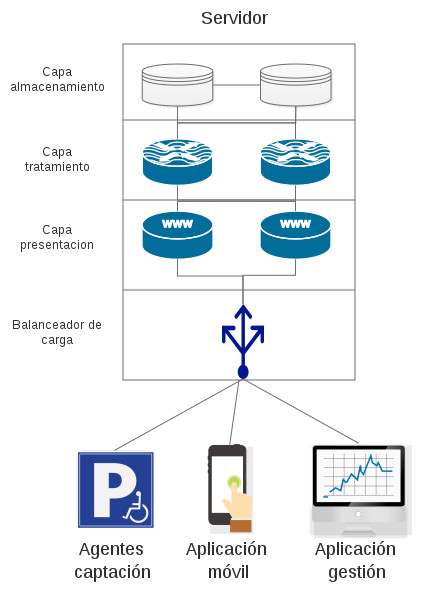
\includegraphics[width=0.5\textwidth]{imagenes/esquema_sistema.jpg}
	\caption{Esquema SGA ideal}
	\label{esquema_sga_ideal}
\end{figure}
\begin{itemize}
	\item en el servidor, ubicado en un centro de procesamiento de datos (CPD), se almacenan, tratan y sirven o reciben datos del resto de dispositivos (parte superior de la figura \ref{esquema_sga_ideal}).
	\item los agentes de captación de datos comprueban el estado de la plaza de aparcamiento y hacen peticiones al servidor para que actualice los datos almacenados en el sistema.
	\item la aplicación móvil muestra al usuario la disponibilidad de los aparcamientos en base a la información almacenada y servida por el servidor.
	\item la aplicación de gestión administra el sistema incluyendo plazas, usuarios, mostrando estadísticas o recibiendo alertas, dependiendo del rol del administrador.
\end{itemize}

\chapter{Planteamiento del problema: objetivos específicos del TFG}
Como se ha visto anteriormente, un sistema ideal automático de gestión de aparcamientos para PMR es lo suficientemente complejo y amplio como para tener que seleccionar parte del mismo para que se pueda desarrollar en el marco de un TFG. En caso contrario, una persona sería incapaz de implementar todas las funcionalidades posibles del sistema en un periodo corto de tiempo. Como se sabe, los créditos del TFG son 12, lo que equivale a unas 300 horas de trabajo.
\\\\
Para ello, sería conveniente seleccionar o simplificar aquellas partes para que el sistema funcione desde un punto de vista global, pudiéndose hacer en un tiempo razonable. Este tiempo no sólo es de implementación sino que, también, se debe dejar un porcentaje bastante elevado del mismo para un análisis exhaustivo precedente a la implantación, ver figura \ref{gantt}.
\\\\
Como se ha visto en el estudio del sistema automático de gestión de aparcamientos para PMR, el sistema se compone de tres capas independientes pero indispensables. Es por ello que durante la implementación de este proyecto se tendrán que hacer partes de las distintas funcionalidades de las tres capas.
\\\\
Por ello, la primera capa, el agente de captación de datos, debería estar incluida en este trabajo final junto a una parte de la tercera, la aplicación móvil del usuario. También, para gestionar el sistema de forma interna, se tendrían que implementar algunas de las funcionalidades de la aplicación para los administradores. Obviamente, la segunda capa, almacenamiento y tratamiento de la información del sistema también debería  crearse. En ella se creará el agente inteligente el cual le buscará al usuario la mejor plaza para estacionar.
\\\\
Funcionalidades como la creación de estadísticas, valoración de las plazas, poder personalizar la búsqueda de plazas…, son consideradas como secundarias en los momentos iniciales de la creación de un proyecto de tal calibre. Por esto, no van a formar parte de los objetivos a implementar en este trabajo.
\\\\
No obstante, y como se ha pensado en dichas funcionalidades, durante la implementación del núcleo inicial de este sistema, se tendrá en cuenta implementar el sistema de tal forma que, a posteriori, sea más fácil la inclusión de nuevas funcionalidades en el mismo.
\\\\
\section{Objetivos específicos}
Por tanto, los objetivos específicos a desarrollar en este TFG serán:
\begin{itemize}
	\item Crear el agente de captación de datos que se dispondrá en las plazas de aparcamiento.
	\item Configurar el sistema de almacenamiento y tratamiento de la información. Para ello se tendrá que elegir cuál sería el mejor sistema gestor de bases de datos (SGBD) para este proyecto.
	\item Crear una aplicación móvil donde localizar las plazas de aparcamiento existentes en el sistema. Dicha aplicación, si se le marca un objetivo, mostrará una lista de las mejores plazas donde aparcar.
	\item Crear una aplicación de escritorio que administre el sistema: añadiendo nuevas plazas, eliminando existentes, añadiendo o eliminando acreditaciones, así como que permita recibir notificaciones sobre una plaza que se encuentre ocupada por un vehículo sin acreditación.
	\item Implementar el sistema para que sea fácil la inclusión de nuevas funcionalidades.
\end{itemize}
Una vez hecha esta delimitación de objetivos en el marco del TFG, se va a proceder a un análisis más formal desde un punto de vista técnico para resolver los objetivos marcados. En este análisis se pondrá de manifiesto las diferentes opciones para realizar un objetivo y, de estas opciones, se elegirá la que se considere mejor para la viabilidad del sistema.
\\\\
Se intentará apostar lo máximo posible por código \textit{open source} y \textit{hardware} igualmente libre para evitar problemas en un futuro venidos por las licencias, aunque la mejor elección pueda ser propietaria. Es por ello que en cada análisis se estudiarán resultados, soporte, comunidad y licencia de la herramienta a usar.
\\\\
Por último, después de haber hecho el análisis correspondiente, se procederá a desarrollar los objetivos en base dicho análisis.
%% así como probar las distintas funcionalidades para asegurar el buen funcionamiento del mismo. Una vez probado las funcionalidades, se procederá a poner en marcha el sistema, llamado despliegue del sistema.
\cleardoublepage 
\chapter{Descripción de la solución propuesta}
Una vez que se sabe qué objetivos son los que se van a implementar en este TFG, lo primero que se debe realizar es un análisis exhaustivo de los mismos. Dicho análisis se va a hacer en base al estándar IEEE Std 830-1998 - IEEE Recommended Practice for Software Requirements Specifications \cite{IEE_830-1998}.
\\\\
Aunque el estándar anterior se remplazó por el estándar IEEE Std 830-1998 - IEEE Recommended Practice for Software Requirements Specifications \cite{IEE_29148-2011} enfocado a metodologías ágiles de creación de software, actualmente se sigue usando el antiguo estándar en multitud de proyectos empresariales y de la Administración Pública. Además, el antiguo es el que se explica en las asignaturas comunes del grado de informática \cite{guia-docente-fis} en esta escuela.
\\\\
A continuación se ha seguido parte del estándar IEEE Std 830-1998 \cite{IEE_830-1998} para analizar los objetivos específicos que se van a implementar en este TFG.
\section{Introducción}
Se va a proceder a la creación del núcleo principal de un sistema automático de gestión de aparcamientos para PMR (personas con movilidad reducida). Dicho sistema ayuda a la gestión de las plazas de aparcamiento, controla el estacionamiento en aquellas plazas que dispongan de sensores, alerta automáticamente cuando una plaza está siendo mal ocupada y guía al usuario a una plaza específica.
\section{Descripción del sistema actual}
Actualmente no existe un sistema automático para el control de plazas para PMR. El control se hace de forma manual y presencial en cada plaza.
\section{Objetivos}
En esta sección se exponen los objetivos del sistema que se quiere desarrollar. Dichos objetivos son:
\\\\
Para crear el sistema automático para el control de plazas para PMR, hay que crear la arquitectura del mismo. Esta arquitectura se ha detallado en el capítulo \ref{arquitectura} pero se detallará para esta solución posteriormente.
\begin{tabularx}{\textwidth}{|l|X|}
	\caption{Objetivo 1 del sistema}\label{OBJ-1}\\
	\hline
	OBJ-1        & Crear arquitectura del sistema \\ \hline
	Versión      & 1 (08/01/2018) \\ \hline
	Autores      & Carlos Cobos \\ \hline
	Descripción  & Se creará la estructura central para alojar al sistema. \\ \hline
	Subobjetivos & 	\begin{tabular}{@{}X@{}}
		OBJ-2 Crear aplicación de gestión (Tabla \ref{OBJ-2}). \\
		OBJ-6 Crear agente de captación de datos (Tabla \ref{OBJ-6}). \\
		OBJ-7 Crear aplicación móvil para el usuario final (Tabla \ref{OBJ-7}).
	\end{tabular} \\ \hline
	Comentarios  & \\ \hline
\end{tabularx}
Administrar el sistema dando de alta plazas de aparcamiento como acreditaciones de aparcamiento a la vez que, para poder recibir notificaciones de las plazas mal utilizadas, es necesario crear una aplicación que lo haga.
\begin{tabularx}{\textwidth}{|l|X|}
	\caption{Objetivo 2 del sistema}\label{OBJ-2}\\
	\hline
	OBJ-2        & Crear aplicación de gestión \\ \hline
	Versión      & 1 (08/01/2018) \\ \hline
	Autores      & Carlos Cobos \\ \hline
	Descripción  & El sistema deberá administrar y gestionar plazas de aparcamiento y acreditaciones. También deberá recibir notificaciones de ocupación de plazas. \\ \hline
	Subobjetivos & 	\begin{tabular}{@{}X@{}}
		OBJ-3 Recepcionar notificaciones (Tabla \ref{OBJ-3}). \\
		OBJ-4 Gestionar plazas de aparcamiento (Tabla \ref{OBJ-4}). \\ 
		OBJ-5 Gestionar acreditaciones de aparcamiento (Tabla \ref{OBJ-5}).
	\end{tabular} \\ \hline
	Comentarios  & \\ \hline
\end{tabularx}

\begin{tabularx}{\textwidth}{|l|X|}
	\caption{Objetivo 3 del sistema}\label{OBJ-3}\\
	\hline
	OBJ-3        & Recepcionar notificaciones \\ \hline
	Versión      & 1 (08/01/2018) \\ \hline
	Autores      & Carlos Cobos \\ \hline
	Descripción  & El sistema deberá notificar a los administradores cuando un vehículo sin autorización estacione en una plaza para PMR. \\ \hline
	Subobjetivos & 	\begin{tabular}{@{}X@{}}
		OBJ-6 Crear agente de captación de datos (Tabla \ref{OBJ-6}).
	\end{tabular} \\ \hline
	Comentarios  & \\ \hline
\end{tabularx}

\begin{tabularx}{\textwidth}{|l|X|}
	\caption{Objetivo 4 del sistema}\label{OBJ-4}\\
	\hline
	OBJ-4        & Gestionar plazas de aparcamiento \\ \hline
	Versión      & 1 (08/01/2018) \\ \hline
	Autores      & Carlos Cobos \\ \hline
	Descripción  & El sistema deberá guardar la información necesaria para la gestión de las distintas plazas de aparcamiento. Además, deberá permitir añadir nuevas plazas de aparcamiento, editar plazas y eliminar plazas existentes en el sistema. \\ \hline
	Subobjetivos & \\ \hline
	Comentarios  & \\ \hline
\end{tabularx}

\begin{tabularx}{\textwidth}{|l|X|}
	\caption{Objetivo 5 del sistema}\label{OBJ-5}\\
	\hline
	OBJ-5        & Gestionar acreditaciones de aparcamiento \\ \hline
	Versión      & 1 (08/01/2018) \\ \hline
	Autores      & Carlos Cobos \\ \hline
	Descripción  & El sistema deberá guardar la información necesaria para registrar los vehículos de aquellas personas que puedan aparcar en las plazas reservadas. Además, deberá permitir añadir nuevas acreditaciones de aparcamiento y eliminar existentes en el sistema. \\ \hline
	Subobjetivos & \\ \hline
	Comentarios  & \\ \hline
\end{tabularx}
Para mantener el sistema con los datos de aparcamiento actualizados es necesario un agente de captación de datos por cada plaza de aparcamiento que se encargue de monitorizar dicha plaza de aparcamiento asociada al agente y actualizar, cuando sea oportuno, los datos del sistema.
\newpage
\begin{tabularx}{\textwidth}{|l|X|}
	\caption{Objetivo 6 del sistema}\label{OBJ-6}\\
	\hline
	OBJ-6        & Crear agente de captación de datos \\ \hline
	Versión      & 1 (08/01/2018) \\ \hline
	Autores      & Carlos Cobos \\ \hline
	Descripción  & El sistema deberá alimentarse de información verídica y en tiempo real de las plazas de aparcamiento a través de agentes de captación de datos. Este va a ser un dispositivo hardware ubicado en las plazas de aparcamiento para PMR. \\ \hline
	Subobjetivos & \\ \hline
	Comentarios  & Éste agente de captación de datos se verá como un usuario que interactúa con el sistema. \\ \hline
\end{tabularx}
Por último, para que los usuarios de este tipo de plazas de aparcamiento se beneficien del sistema, se deberá crear una aplicación móvil para este tipo de usuarios donde poder ver y buscar una plaza de aparcamiento.
\begin{tabularx}{\textwidth}{|l|X|}
	\caption{Objetivo 7 del sistema}\label{OBJ-7}\\
	\hline
	OBJ-7        & Crear aplicación móvil para el usuario final \\ \hline
	Versión      & 1 (08/01/2018) \\ \hline
	Autores      & Carlos Cobos \\ \hline
	Descripción  & El sistema deberá servir información de plazas al usuario final. También deberá guiarle a plazas disponibles. \\ \hline
	Subobjetivos & 	\begin{tabular}{@{}X@{}}
		OBJ-8 Buscar plazas de aparcamiento (Tabla \ref{OBJ-8}).
	\end{tabular} \\ \hline
	Comentarios  & Este agente de captación de datos se verá como un usuario que interactúa con el sistema. \\ \hline
\end{tabularx}

\begin{tabularx}{\textwidth}{|l|X|}
	\caption{Objetivo 8 del sistema}\label{OBJ-8}\\
	\hline
	OBJ-8        & Buscar plazas de aparcamiento \\ \hline
	Versión      & 1 (08/01/2018) \\ \hline
	Autores      & Carlos Cobos \\ \hline
	Descripción  & El sistema deberá encontrar plazas de aparcamiento dado el destino del usuario final en base a la ocupación de las mismas. \\ \hline
	Subobjetivos & \\ \hline
	Comentarios  & \\ \hline
\end{tabularx}

\newpage
\section{Catálogo de requisitos del sistema}
Una vez que se han definido los objetivos globales del sistema, se va a proceder a definir qué información necesita guardar para funcionar correctamente, así como quién y cómo interactúa con el mismo.

\subsection{Requisitos de información}
Los requisitos de información describen qué tipo de información tiene que guardar el sistema para hacer frente a los objetivos marcados anteriormente. \\

\begin{tabularx}{\textwidth}{|l|X|}
	\caption{Requisito 1 de información del sistema}\label{IRQ-1}\\
	\hline
	IRQ-1                & Datos plaza de aparcamiento \\ \hline
	Versión              & 1 (09/01/2018) \\ \hline
	Autores              & Carlos Cobos \\ \hline
	Objetivos asociados  & 	{\begin{tabular}{@{}X@{}}
								OBJ-4 Gestionar plazas de aparcamiento (Tabla \ref{OBJ-4}).
							\end{tabular}} \\ \hline
	Requisitos asociados & IRQ-2 Datos ubicación de aparcamiento \\ \hline
	Descripción          & El sistema deberá almacenar la información correspondiente a las plazas de aparcamiento. En concreto: ubicación y estado actual. \\ \hline
	Datos específicos    & 	{\begin{tabular}{@{}X@{}}
								Puede haber más de una plaza con la misma ubicación. \\
								Ubicación: identificador de ubicación. \\
								Estado: número entero. -1 no definido, 0 disponible, 1 ocupada, 2 mal ocupada.
							\end{tabular}} \\ \hline
	Comentarios  & \\ \hline
\end{tabularx}

\begin{tabularx}{\textwidth}{|l|X|}
	\caption{Requisito 2 de información del sistema}\label{IRQ-2}\\
	\hline
	IRQ-2                & Datos ubicación de aparcamiento \\ \hline
	Versión              & 1 (09/01/2018) \\ \hline
	Autores              & Carlos Cobos \\ \hline
	Objetivos asociados  & 	\begin{tabular}{@{}X@{}}
		OBJ-4 Gestionar plazas de aparcamiento (Tabla \ref{OBJ-4}).
	\end{tabular} \\ \hline
	Requisitos asociados &  \\ \hline
	Descripción          & El sistema deberá almacenar la información correspondiente a las ubicaciones de las plazas de aparcamiento. En concreto: dirección, restricciones y plazas en dicha ubicación. \\ \hline
	Datos específicos    & 	{\begin{tabular}{@{}X@{}}
			Además de almacenar la calle y el número en la dirección, se debería almacenar su latitud y longitud (posición GPS) para geoposicionarla en un mapa. \\
			En algunas plazas hay restricciones horarias o posibilidad de que aparquen otros vehículos. \\
			Dirección: cadena de caracteres. Calle y número. \\
			Latitud: número decimal. \\
			Longitud: numero decimal. \\
			Restricciones: cadena compleja. \\
			Número de plazas totales: número entero.
	\end{tabular}} \\ \hline
	Comentarios  & \\ \hline
\end{tabularx}

\begin{tabularx}{\textwidth}{|l|X|}
	\caption{Requisito 3 de información del sistema}\label{IRQ-3}\\
	\hline
	IRQ-3                & Datos acreditación de aparcamiento \\ \hline
	Versión              & 1 (09/01/2018) \\ \hline
	Autores              & Carlos Cobos \\ \hline
	Objetivos asociados  & 	\begin{tabular}{@{}X@{}}
		OBJ-5 Gestionar acreditaciones de aparcamiento (Tabla \ref{OBJ-5}).
	\end{tabular} \\ \hline
	Requisitos asociados &  \\ \hline
	Descripción          & El sistema deberá almacenar la información correspondiente a las acreditaciones de aparcamiento. En concreto: identificador de acreditación. \\ \hline
	Datos específicos    & 	{\begin{tabular}{@{}X@{}}
			Cada acreditación pertenece a una persona registrada en un sistema externo. \\
			Una persona física solamente puede poseer una acreditación activa.\\
			Identificador acreditación: número entero. Normalmente almacenado en hexadecimal.
	\end{tabular}} \\ \hline
	Comentarios  & \\ \hline
\end{tabularx}

\newpage
\begin{tabularx}{\textwidth}{|l|X|}
	\caption{Requisito 4 de información del sistema}\label{IRQ-4}\\
	\hline
	IRQ-4                & Registro de utilización de plazas \\ \hline
	Versión              & 1 (09/01/2018) \\ \hline
	Autores              & Carlos Cobos \\ \hline
	Objetivos asociados  & 	{\begin{tabular}{@{}X@{}}
		OBJ-4 Gestionar plazas de aparcamiento (Tabla \ref{OBJ-4}). \\
		OBJ-6 Crear agente de captación de datos (Tabla \ref{OBJ-6}). \\
		OBJ-8 Buscar mejores plazas de aparcamiento (Tabla \ref{OBJ-8}). \\
		OBJ-FUTURO Preparación de datos para estadísticas de plazas.
	\end{tabular}} \\ \hline
	Requisitos asociados &  \\ \hline
	Descripción          & El sistema deberá almacenar la información correspondiente al estado de las plazas en el transcurso del tiempo. \\ \hline
	Datos específicos    & 	{\begin{tabular}{@{}X@{}}
			Se almacenará el identificador de la plaza junto al nuevo estado que haya tomado y la fecha y hora cuando una plaza cambie de estado. \\
			El agente de captación de datos notificará al sistema cuando ocurra un cambio de estado en su plaza. \\
			Identificador de plaza: número entero. \\
			Estado: número entero. -1 no definido, 0 disponible, 1 ocupada, 2 mal ocupada. \\
			Tiempo: marca de tiempo (fecha y hora).
	\end{tabular}} \\ \hline
	Comentarios  & \\ \hline
\end{tabularx}

\begin{tabularx}{\textwidth}{|l|X|}
	\caption{Requisito 5 de información del sistema}\label{IRQ-5}\\
	\hline
	IRQ-5                & Registro de destino de usuarios \\ \hline
	Versión              & 1 (09/01/2018) \\ \hline
	Autores              & Carlos Cobos \\ \hline
	Objetivos asociados  & 	{\begin{tabular}{@{}X@{}}
			OBJ-8 Buscar mejores plazas de aparcamiento (Tabla \ref{OBJ-8}). \\
			OBJ-FUTURO Preparación de datos para estadísticas de plazas. \\
			OBJ-FUTURO Preparación de datos para estadísticas de destino.
	\end{tabular}} \\ \hline
	Requisitos asociados &  \\ \hline
	Descripción          & El sistema deberá almacenar la información correspondiente al destino de los usuarios. \\ \hline
	Datos específicos    & 	{\begin{tabular}{@{}X@{}}
			Se almacenará el destino que busca un usuario junto a la marca de tiempo en el que se ha producido la búsqueda. \\
			Latitud: número decimal. Latitud del destino final del usuario. \\
			Longitud: numero decimal. Longitud del destino final del usuario. \\
			Tiempo: marca de tiempo (fecha y hora). 
	\end{tabular}} \\ \hline
	Comentarios  & Por ahora y debido a que una acreditación representa únicamente a un usuario, se tomará el identificador de la acreditación como el del usuario. \\ \hline
\end{tabularx}

\begin{tabularx}{\textwidth}{|l|X|}
	\caption{Requisito 6 de información del sistema}\label{IRQ-6}\\
	\hline
	IRQ-6                & Destino activo \\ \hline
	Versión              & 1 (09/01/2018) \\ \hline
	Autores              & Carlos Cobos \\ \hline
	Objetivos asociados  & 	{\begin{tabular}{@{}X@{}}
			OBJ-7 Crear aplicación móvil para el usuario final (Tabla \ref{OBJ-7}). \\
			OBJ-8 Buscar mejores plazas de aparcamiento (Tabla \ref{OBJ-8}). \\
	\end{tabular}} \\ \hline
	Requisitos asociados &  \\ \hline
	Descripción          & Para que el sistema sepa a quién notificar al ocuparse una plaza de aparcamiento, deberá almacenar la información correspondiente a la ubicación de destino de los usuarios de la aplicación móvil desde el momento que inicia la navegación a dicha ubicación hasta que llega al destino o interrumpe la navegación. \\ \hline
	Datos específicos    & 	{\begin{tabular}{@{}X@{}}
			Identificador de la aplicación móvil del usuario: número entero. \\
			Identificador de la ubicación de destino: número entero. \\
	\end{tabular}} \\ \hline
	Comentarios  & Dicha información sirve para avisar al posible usuario, que está navegando a una ubicación determinada, si la última plaza libre de ésta se ha ocupado. \\ \hline
\end{tabularx}

\newpage
\subsubsection{Requisitos funcionales}
Los requisitos funcionales describen las acciones del sistema. Para que pueda realizar algunas de las mismas, se tiene que definir a los usuarios que interactúan con éste. Estos usuarios, en adelante actores, ordenan lo que el sistema tiene que hacer pidiendo datos que el actor tiene que introducir. A esta interacción se le llama \textit{caso de uso}.
\begin{tabularx}{\textwidth}{|l|X|}
	\caption{Requisito funcional 1 del sistema}\label{FR-1}\\
	\hline
	FR-1        & Administrar ubicaciones de aparcamiento \\ \hline
	Versión     & 1 (10/01/2018) \\ \hline
	Autores     & Carlos Cobos \\ \hline
	Descripción & Los administradores deberán dar de alta, modificar o eliminar ubicaciones del sistema. \\ \hline
	Comentarios &  \\ \hline
\end{tabularx}

\begin{tabularx}{\textwidth}{|l|X|}
	\caption{Requisito funcional 2 del sistema}\label{FR-2}\\
	\hline
	FR-2        & Administrar plazas de aparcamiento \\ \hline
	Versión     & 1 (10/01/2018) \\ \hline
	Autores     & Carlos Cobos \\ \hline
	Descripción & Los administradores deberán dar de alta o de baja plazas de las ubicaciones del sistema. \\ \hline
	Comentarios &  \\ \hline
\end{tabularx}

\begin{tabularx}{\textwidth}{|l|X|}
	\caption{Requisito funcional 3 del sistema}\label{FR-3}\\
	\hline
	FR-3        & Administrar acreditaciones de aparcamiento \\ \hline
	Versión     & 1 (10/01/2018) \\ \hline
	Autores     & Carlos Cobos \\ \hline
	Descripción & Los administradores deberán dar de alta o de baja acreditaciones de aparcamiento del sistema. \\ \hline
	Comentarios &  \\ \hline
\end{tabularx}

\begin{tabularx}{\textwidth}{|l|X|}
	\caption{Requisito funcional 4 del sistema}\label{FR-4}\\
	\hline
	FR-4        & Actualizar estado de las plazas \\ \hline
	Versión     & 1 (10/01/2018) \\ \hline
	Autores     & Carlos Cobos \\ \hline
	Descripción & Los agentes de captación deberán actualizar la plaza asociada en el sistema. \\ \hline
	Comentarios &  \\ \hline
\end{tabularx}

\newpage
\begin{tabularx}{\textwidth}{|l|X|}
	\caption{Requisito funcional 5 del sistema}\label{FR-5}\\
	\hline
	FR-5        & Gestionar notificaciones \\ \hline
	Versión     & 1 (10/01/2018) \\ \hline
	Autores     & Carlos Cobos \\ \hline
	Descripción & Los administradores deberán recibir un aviso cuando una plaza sea mal usada. Por su parte, el usuario deberá recibir un aviso cuando se ocupen todas las plazas de la ubicación a la que se dirige. \\ \hline
	Comentarios &  \\ \hline
\end{tabularx}

\begin{tabularx}{\textwidth}{|l|X|}
	\caption{Requisito funcional 6 del sistema}\label{FR-6}\\
	\hline
	FR-6        & Buscar plazas \\ \hline
	Versión     & 1 (10/01/2018) \\ \hline
	Autores     & Carlos Cobos \\ \hline
	Descripción & El sistema deberá mostrar una lista de ubicaciones donde se pueda aparcar dada una posición. \\ \hline
	Comentarios &  \\ \hline
\end{tabularx}

\begin{tabularx}{\textwidth}{|l|X|}
	\caption{Requisito funcional 7 del sistema}\label{FR-7}\\
	\hline
	FR-7        & Navegar a plazas de aparcamiento \\ \hline
	Versión     & 1 (10/01/2018) \\ \hline
	Autores     & Carlos Cobos \\ \hline
	Descripción & El sistema deberá guiar al usuario a una ubicación de aparcamiento. \\ \hline
	Comentarios &  \\ \hline
\end{tabularx}

\newpage
\subsubsection{Definición de los actores}
\begin{tabularx}{\textwidth}{|l|X|}
	\caption{Actor 1 del sistema}\label{ACT-1}\\
	\hline
	ACT-1       & Usuario final \\ \hline
	Versión     & 1 (10/01/2018) \\ \hline
	Autores     & Carlos Cobos \\ \hline
	Descripción & Este actor representa al usuario final del sistema que desea hacer uso de las plazas monitorizadas. \\ \hline
	Comentarios & Este actor hará uso del sistema a través de una aplicación móvil cuando se encuentre en el vehículo. \\ \hline
\end{tabularx}

\begin{tabularx}{\textwidth}{|l|X|}
	\caption{Actor 2 del sistema}\label{ACT-2}\\
	\hline
	ACT-2       & Administrador \footnotemark \\ \hline
	Versión     & 1 (10/01/2018) \\ \hline
	Autores     & Carlos Cobos \\ \hline
	Descripción & Este actor representa a varios de los posibles administradores en un futuro. Este actor podrá gestionar todo el sistema. \\ \hline
	Comentarios & Este actor hará uso del sistema a través de una aplicación de escritorio. \\ \hline
\end{tabularx}

\footnotetext{En un futuro, este actor de dividirá en tres: agentes de administración local, agentes de la autoridad local y agentes de la administración regional.}
\begin{tabularx}{\textwidth}{|l|X|}
	\caption{Actor 3 del sistema}\label{ACT-3}\\
	\hline
	ACT-3       & Agente de captación de datos \\ \hline
	Versión     & 1 (10/01/2018) \\ \hline
	Autores     & Carlos Cobos \\ \hline
	Descripción & Este actor representa a los dispositivos que se colocarán en las plazas de aparcamiento para proveer al sistema de datos. \\ \hline
	Comentarios & Este actor será un dispositivo electrónico. \\ \hline
\end{tabularx}

\newpage
\subsubsection{Casos de uso}
%\begin{figure}[H]
%	\centering
%	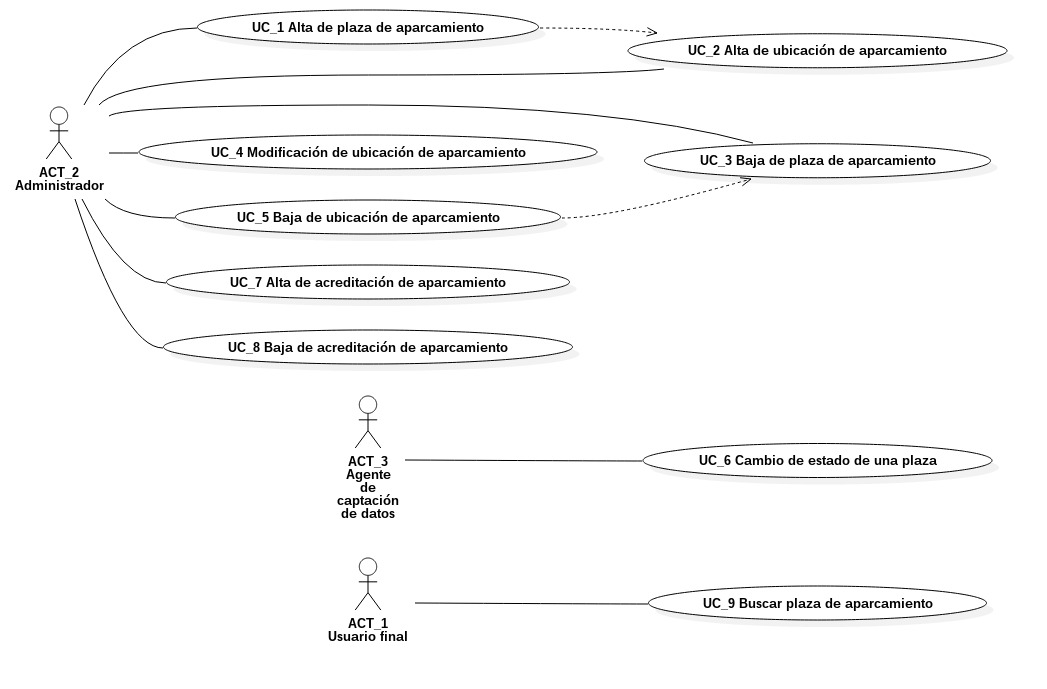
\includegraphics[width=\textwidth]{imagenes/casos_de_uso.jpg}
%	\caption{Esquema casos de uso}
%	\label{esquema_UC}
%\end{figure}

\begin{sidewaysfigure}[H]
	\centering
	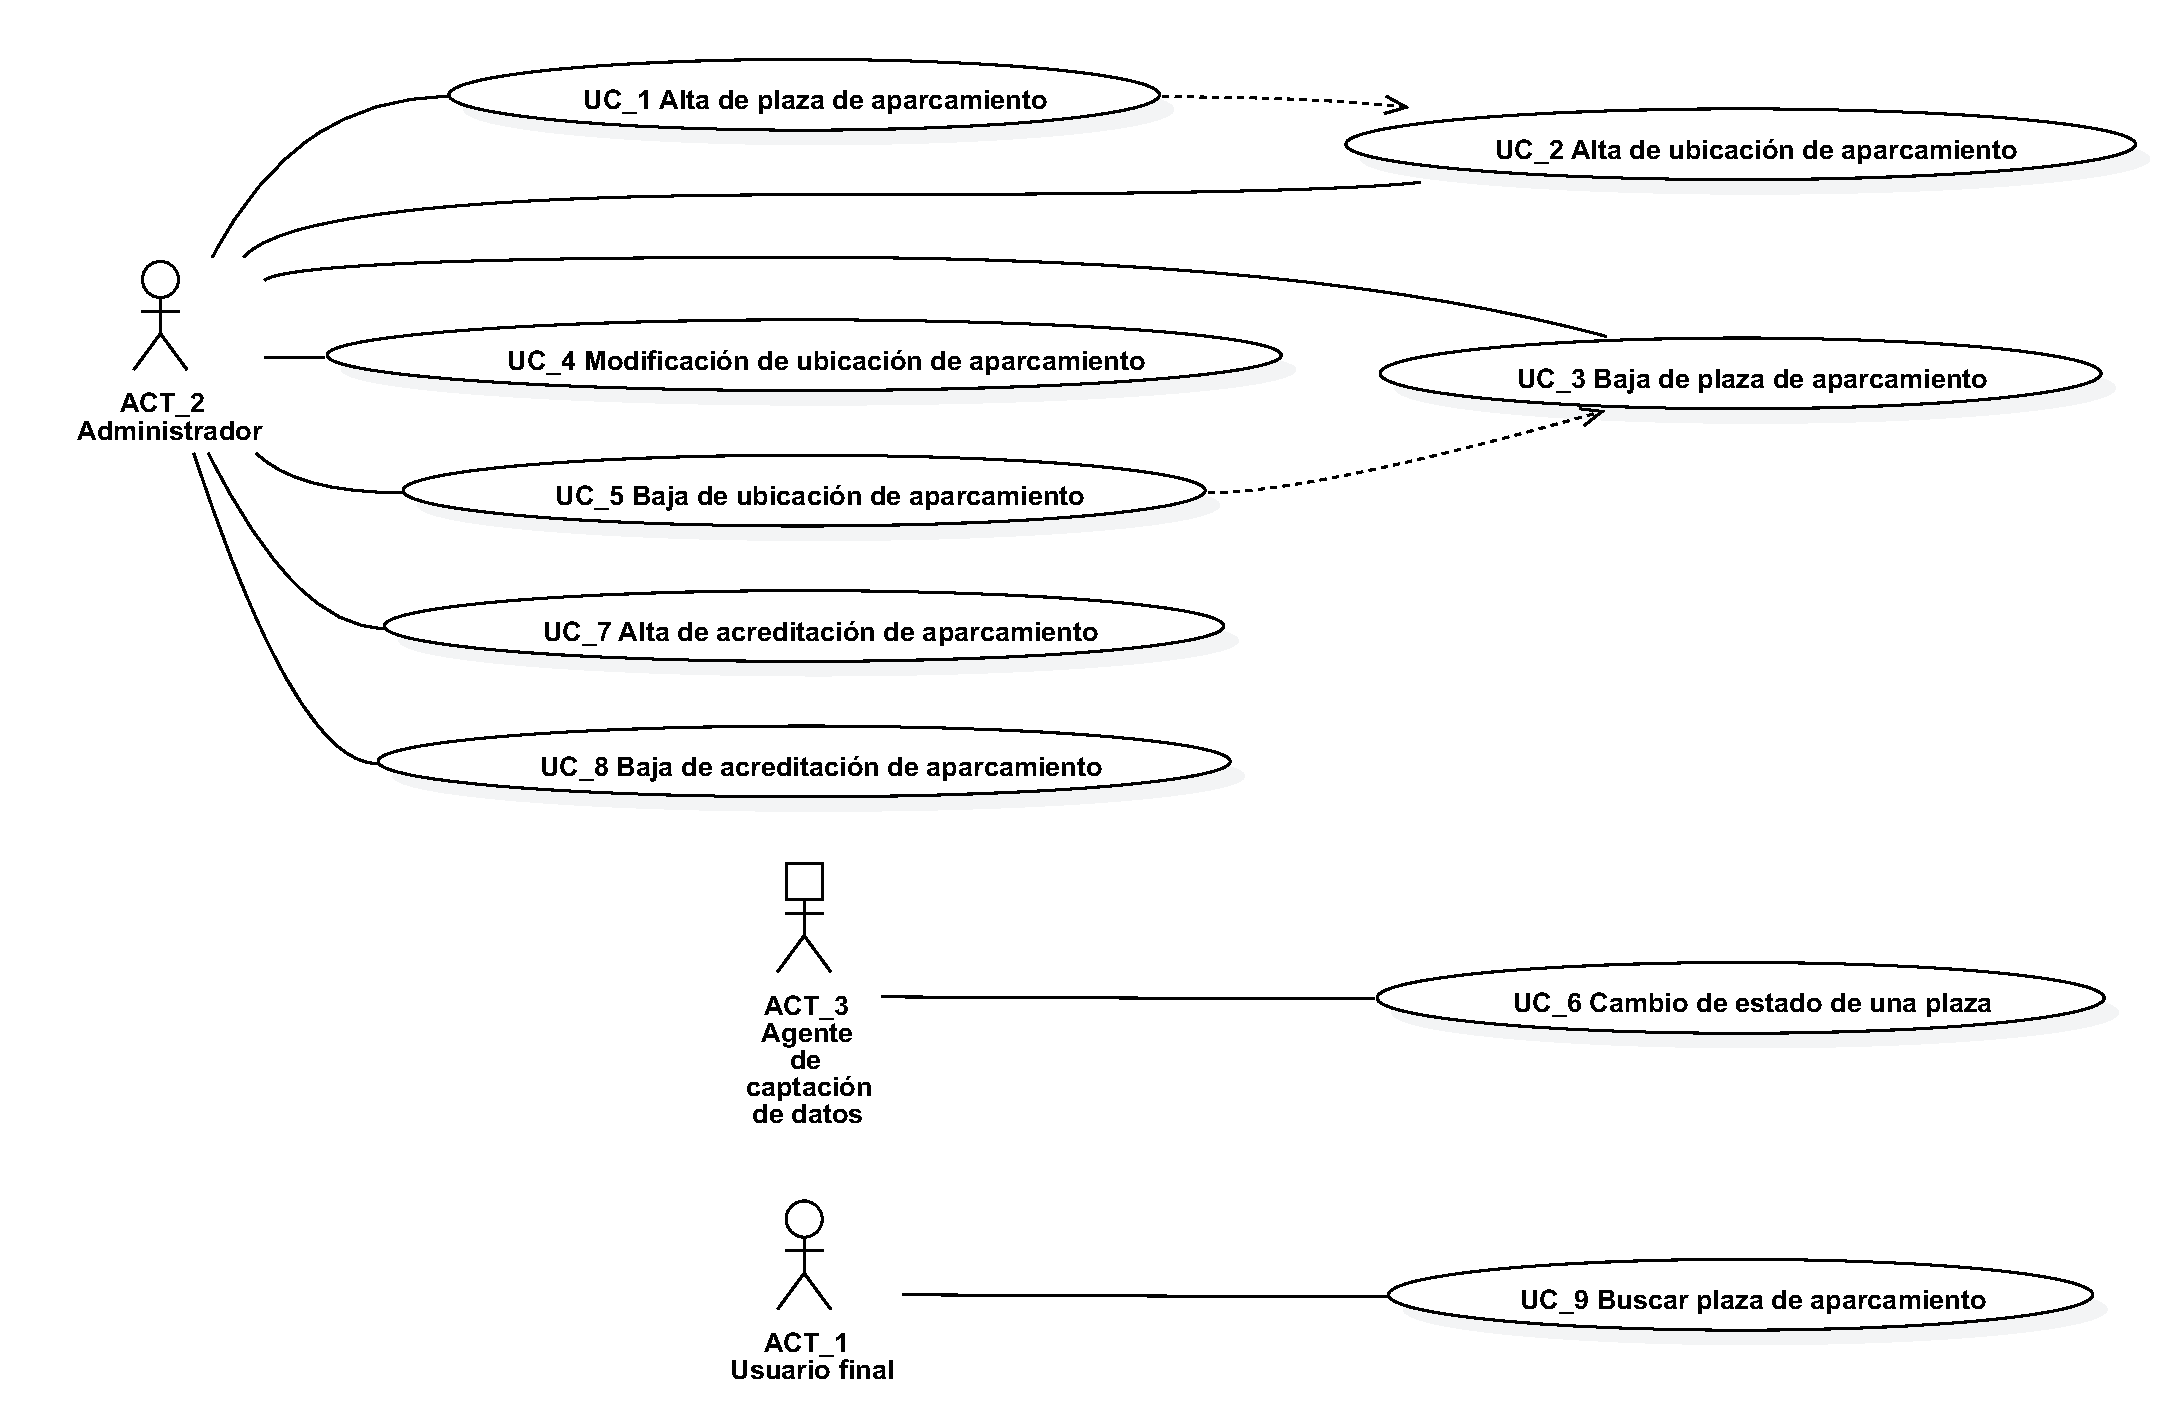
\includegraphics[width=\textwidth]{imagenes/casos_de_uso.eps}
	\caption{Esquema casos de uso}
	\label{esquema_UC}
\end{sidewaysfigure}

\begin{tabularx}{\textwidth}{|l|X|}
	\caption{Caso de uso 1 del sistema}\label{UC-1}\\
	\hline
	UC-1                 & Alta de plaza de aparcamiento \\ \hline
	Versión              & 1 (10/01/2018) \\ \hline
	Autores              & Carlos Cobos \\ \hline
	Objetivos asociados  & OBJ-4 Gestionar plazas de aparcamiento (Tabla \ref{OBJ-4} \\ \hline
	Requisitos asociados &  {\begin{tabular}{@{}X@{}}
									IRQ-1 Datos plaza de aparcamiento (Tabla \ref{IRQ-1}) \\
									IRQ-2 Datos ubicación de aparcamiento (Tabla \ref{IRQ-2}) \\
									FR-2 Administrar plazas de aparcamiento (Tabla \ref{FR-2}) \\
							\end{tabular}} \\ \hline
	Descripción          & El sistema deberá pedir los datos necesarios al administrador para añadir una nueva plaza de aparcamiento en el sistema. \\ \hline
	Precondición         &  \\ \hline
	Secuencia normal     & 	{\begin{tabular}{@{}l|p{\anchoColumna{}}@{}}
								Paso & Acción \\ \hline
								1 & El actor administrador inserta un identificador de una ubicación. \\ \hline
								2 & El sistema añade una plaza a la ubicación dada. \\ \hline
								3 & El sistema actualiza el número de plazas de la ubicación dada. \\
							\end{tabular}} \\ \hline
	Postcondición        &  \\ \hline
	Excepciones          & 	{\begin{tabular}{@{}l|p{\anchoColumna{}}@{}}
								Paso & Acción \\ \hline
								1 & Si la ubicación de la nueva plaza no existe, se realizará el caso de uso UC-2 (Tabla \ref{UC-2}). \\
							\end{tabular}} \\ \hline
\end{tabularx}

\begin{tabularx}{\textwidth}{|l|X|}
	\caption{Caso de uso 2 del sistema}\label{UC-2}\\
	\hline
	UC-2                 & Alta de ubicación de aparcamiento \\ \hline
	Versión              & 1 (10/01/2018) \\ \hline
	Autores              & Carlos Cobos \\ \hline
	Objetivos asociados  & 	{\begin{tabular}{@{}X@{}}
			OBJ-4 Gestionar plazas de aparcamiento (Tabla \ref{OBJ-4}) \\
	\end{tabular}} \\ \hline
	Requisitos asociados &  {\begin{tabular}{@{}X@{}}
			IRQ-2 Datos ubicación de aparcamiento (Tabla \ref{IRQ-2}) \\
			FR-2 Administrar plazas de aparcamiento (Tabla \ref{FR-2}) \\
	\end{tabular}} \\ \hline
	Descripción          & El sistema deberá pedir los datos necesarios al administrador para añadir una nueva ubicación de aparcamiento en el sistema. \\ \hline
	Precondición         &  \\ \hline
	Secuencia normal     & 	{\begin{tabular}{@{}l|p{\anchoColumna{}}@{}}
			Paso & Acción \\ \hline
			1 & El actor administrador introduce una dirección, una posición GPS (latitud y longitud) y unas restricciones a la ubicación si precede. \\ \hline
			2 & El sistema añade la nueva ubicación con número de plazas a 0. \\
	\end{tabular}} \\ \hline
	Postcondición        &  \\ \hline
	Excepciones          & 	{\begin{tabular}{@{}l|p{\anchoColumna{}}@{}}
			Paso & Acción \\ \hline
			1 & Si la posición GPS de la plaza es igual que la de una plaza existente en el sistema, no se procederá.
	\end{tabular}} \\ \hline
\end{tabularx}

\begin{tabularx}{\textwidth}{|l|X|}
	\caption{Caso de uso 3 del sistema}\label{UC-3}\\
	\hline
	UC-3                 & Baja de plaza de aparcamiento \\ \hline
	Versión              & 1 (10/01/2018) \\ \hline
	Autores              & Carlos Cobos \\ \hline
	Objetivos asociados  & 	{\begin{tabular}{@{}X@{}}
			OBJ-4 Gestionar plazas de aparcamiento (Tabla \ref{OBJ-4}) \\
	\end{tabular}} \\ \hline
	Requisitos asociados &  {\begin{tabular}{@{}X@{}}
			IRQ-1 Datos plaza de aparcamiento (Tabla \ref{IRQ-1}) \\
			IRQ-2 Datos ubicación de aparcamiento (Tabla \ref{IRQ-2}) \\
			FR-2 Administrar plazas de aparcamiento (Tabla \ref{FR-2}) \\
	\end{tabular}} \\ \hline
	Descripción          & El sistema deberá pedir los datos necesarios al administrador para eliminar una plaza de aparcamiento en el sistema. \\ \hline
	Precondición         &  \\ \hline
	Secuencia normal     & 	{\begin{tabular}{@{}l|p{\anchoColumna{}}@{}}
			Paso & Acción \\ \hline
			1 & El actor administrador inserta un identificador de una plaza. \\ \hline
			2 & El sistema elimina la plaza seleccionada. \\ \hline
			3 & El sistema actualiza el número de plazas de la ubicación asociada. \\
	\end{tabular}} \\ \hline
	Postcondición        &  \\ \hline
	Excepciones          & 	{\begin{tabular}{@{}l|p{\anchoColumna{}}@{}}
			Paso & Acción \\ \hline
			1 & Si el identificador de la plaza no existe, no se procederá. \\ 
	\end{tabular}} \\ \hline
\end{tabularx}

\newpage
\begin{tabularx}{\textwidth}{|l|X|}
	\caption{Caso de uso 4 del sistema}\label{UC-4}\\
	\hline
	UC-4                 & Modificación de ubicación de aparcamiento \\ \hline
	Versión              & 1 (10/01/2018) \\ \hline
	Autores              & Carlos Cobos \\ \hline
	Objetivos asociados  & 	{\begin{tabular}{@{}X@{}}
			OBJ-4 Gestionar plazas de aparcamiento (Tabla \ref{OBJ-4}) \\
	\end{tabular}} \\ \hline
	Requisitos asociados &  {\begin{tabular}{@{}X@{}}
			IRQ-2 Datos ubicación de aparcamiento (Tabla \ref{IRQ-2}) \\
			FR-1 Administrar ubicaciones de aparcamiento (Tabla \ref{FR-1}) \\
	\end{tabular}} \\ \hline
	Descripción          & El sistema deberá permitir modificar algunos campos de la ubicación de plazas. \\ \hline
	Precondición         &  \\ \hline
	Secuencia normal     & 	{\begin{tabular}{@{}l|p{\anchoColumna{}}@{}}
			Paso & Acción \\ \hline
			1 & El actor administrador inserta un identificador de una ubicación. \\ \hline
			2 & El sistema muestra la información asociada a dicha ubicación. \\ \hline
			3 & El actor administrador podrá modificar la dirección y las restricciones de la ubicación. \\ \hline
			4 & El sistema almacenará la nueva información. \\
	\end{tabular}} \\ \hline
	Postcondición        &  \\ \hline
	Excepciones          & 	{\begin{tabular}{@{}l|p{\anchoColumna{}}@{}}
			Paso & Acción \\ \hline
			1 & Si el identificador de la ubicación no existe, no se procederá. \\ 
	\end{tabular}} \\ \hline
\end{tabularx}

\begin{tabularx}{\textwidth}{|l|X|}
	\caption{Caso de uso 5 del sistema}\label{UC-5}\\
	\hline
	UC-5                 & Baja de ubicación de aparcamiento \\ \hline
	Versión              & 1 (10/01/2018) \\ \hline
	Autores              & Carlos Cobos \\ \hline
	Objetivos asociados  & 	{\begin{tabular}{@{}X@{}}
			OBJ-4 Gestionar plazas de aparcamiento (Tabla \ref{OBJ-4}) \\
	\end{tabular}} \\ \hline
	Requisitos asociados &  {\begin{tabular}{@{}X@{}}
			IRQ-2 Datos ubicación de aparcamiento (Tabla \ref{IRQ-2}) \\
			FR-1 Administrar ubicaciones de aparcamiento (Tabla \ref{FR-1}) \\
	\end{tabular}} \\ \hline
	Descripción          & El sistema deberá permitir eliminar una ubicación de plazas. \\ \hline
	Precondición         &  \\ \hline
	Secuencia normal     & 	{\begin{tabular}{@{}l|p{\anchoColumna{}}@{}}
			Paso & Acción \\ \hline
			1 & El actor administrador inserta un identificador de una ubicación. \\ \hline
			2 & El sistema muestra la información asociada a dicha ubicación. \\ \hline
			3 & El actor administrador confirmará la ubicación. \\ \hline
			4 & El sistema eliminará la ubicación. \\ 
	\end{tabular}} \\ \hline
	Postcondición        &  \\ \hline
	Excepciones          & 	{\begin{tabular}{@{}l|p{\anchoColumna{}}@{}}
			Paso & Acción \\ \hline
			1 & Si el identificador de la ubicación no existe, no se procederá. \\ \hline
			3 & Si el número de plazas totales de la ubicación es mayor de 0, no se procederá. \\
	\end{tabular}} \\ \hline
\end{tabularx}

\begin{tabularx}{\textwidth}{|l|X|}
	\caption{Caso de uso 6 del sistema}\label{UC-6}\\
	\hline
	UC-6                 & Cambio de estado de una plaza \\ \hline
	Versión              & 1 (10/01/2018) \\ \hline
	Autores              & Carlos Cobos \\ \hline
	Objetivos asociados  & 	{\begin{tabular}{@{}X@{}}
			OBJ-3 Recepcionar notificaciones (Tabla \ref{OBJ-3}) \\
			OBJ-4 Gestionar plazas de aparcamiento (Tabla \ref{OBJ-4}) \\
			OBJ-6 Crear agente de captación de datos (Tabla \ref{OBJ-6})
	\end{tabular}} \\ \hline
	Requisitos asociados &  {\begin{tabular}{@{}X@{}}
			IRQ-1 Datos plaza de aparcamiento (Tabla \ref{IRQ-1}) \\
			IRQ-2 Datos ubicación de aparcamiento (Tabla \ref{IRQ-2}) \\
			IRQ-3 Datos acreditación de aparcamiento (Tabla \ref{IRQ-3}) \\
			IRQ-4 Registro de utilización de plazas (Tabla \ref{IRQ-4}) \\
			IRQ-6 Destino activo (Tabla \ref{IRQ-3}) \\
			FR-4 Actualizar estado de las plazas (Tabla \ref{FR-4}) \\
			FR-5 Gestionar notificaciones (Tabla \ref{FR-5}) \\
	\end{tabular}} \\ \hline
	Descripción          & Cuando el agente de captación de datos detecte un cambio de estado en su plaza, el sistema deberá almacenar dicho estado y actuar en consecuencia. \\ \hline
	Precondición         &  \\ \hline
	Secuencia normal     & 	{\begin{tabular}{@{}l|p{\anchoColumna{}}@{}}
			Paso & Acción \\ \hline
			1 & El agente de captación de datos detecta un cambio de estado en su plaza. \\ \hline
			2 & {\begin{tabular}{@{}l|p{\anchoColumnaInterior{}}@{}}
					& Si la plaza se ha quedado libre. \\ \hline
					2.1 & El sistema actualiza los datos de la plaza de aparcamiento. \\ \hline
					2.2 & El sistema actualiza los datos del registro de utilización de la plaza de aparcamiento. \\
				\end{tabular}} \\ \hline
			3 & {\begin{tabular}{@{}l|p{\anchoColumnaInterior{}}@{}}
					& Si la plaza se ha quedado ocupada. \\ \hline
					3.1 & El sistema lee la acreditación del vehículo. \\ \hline
					3.2 & {\begin{tabular}{@{}l|p{\anchoColumnaMasInterior{}}@{}}
							& El sistema comprueba que la plaza no esté en el registro de destino activo. \\ \hline
							3.2.1 & Si está, se notifica a la aplicación móvil asociada. \\
						\end{tabular}} \\ 
					3.3 & El sistema comprueba que la acreditación leída existe. \\ \hline
					3.4 & El sistema actualiza los datos de la plaza de aparcamiento. \\ \hline
					3.5 & El sistema actualiza los datos del registro de utilización de la plaza de aparcamiento. \\
				\end{tabular}} \\ 
	\end{tabular}} \\ \hline
	Postcondición        &  \\ \hline
	Excepciones          & 	{\begin{tabular}{@{}l|p{\anchoColumna{}}@{}}
			Paso & Acción \\ \hline
			3.1 & {\begin{tabular}{@{}l|p{\anchoColumnaInterior{}}@{}}
					& No se detecta acreditación del vehículo. \\ \hline
					1 & Se notifica a la aplicación de administración sobre la incidencia. \\ \hline
					2 & El sistema actualiza los datos de la plaza de aparcamiento con estado mal ocupado. \\ \hline
					3 & El sistema actualiza los datos del registro de utilización de la plaza de aparcamiento. \\
				\end{tabular}} \\ \hline
			3.3 & {\begin{tabular}{@{}l|p{\anchoColumnaInterior{}}@{}}
					& La acreditación leída no existe en el sistema. \\ \hline
					1 & Se notifica a la aplicación de administración sobre la incidencia. \\ \hline
					2 & El sistema actualiza los datos de la plaza de aparcamiento con estado mal ocupado. \\ \hline
					3 & El sistema actualiza los datos del registro de utilización de la plaza de aparcamiento. \\
			\end{tabular}}
	\end{tabular}} \\ \hline
\end{tabularx}

\begin{tabularx}{\textwidth}{|l|X|}
	\caption{Caso de uso 7 del sistema}\label{UC-7}\\
	\hline
	UC-7                 & Alta de acreditación de aparcamiento \\ \hline
	Versión              & 1 (10/01/2018) \\ \hline
	Autores              & Carlos Cobos \\ \hline
	Objetivos asociados  & 	{\begin{tabular}{@{}X@{}}
			OBJ-5 Gestionar acreditaciones de aparcamiento (Tabla \ref{OBJ-5}) \\
	\end{tabular}} \\ \hline
	Requisitos asociados &  {\begin{tabular}{@{}X@{}}
			IRQ-3 Datos acreditación de aparcamiento (Tabla \ref{IRQ-3}) \\
			FR-3 Administrar acreditaciones de aparcamiento (Tabla \ref{FR-3}) \\
	\end{tabular}} \\ \hline
	Descripción          & El sistema deberá pedir los datos necesarios al administrador para añadir una nueva acreditación de aparcamiento en el sistema. \\ \hline
	Precondición         & Identificador de la nueva acreditación no existe en el sistema. \\ \hline
	Secuencia normal     & 	{\begin{tabular}{@{}l|p{\anchoColumna{}}@{}}
			Paso & Acción \\ \hline
			1 & El actor administrador introduce un nuevo identificador único de acreditación. \\ \hline
			2 & El sistema añade la nueva acreditación. \\
	\end{tabular}} \\ \hline
	Postcondición        &  \\ \hline
	Excepciones          & 	{\begin{tabular}{@{}l|p{\anchoColumna{}}@{}}
			Paso & Acción \\ \hline
			1 & Si la posición GPS de la plaza es igual que la de una plaza existente en el sistema, no se procederá.
	\end{tabular}} \\ \hline
\end{tabularx}

\begin{tabularx}{\textwidth}{|l|X|}
	\caption{Caso de uso 8 del sistema}\label{UC-8}\\
	\hline
	UC-8                 & Baja de acreditación de aparcamiento \\ \hline
	Versión              & 1 (10/01/2018) \\ \hline
	Autores              & Carlos Cobos \\ \hline
	Objetivos asociados  & 	{\begin{tabular}{@{}X@{}}
			OBJ-5 Gestionar acreditaciones de aparcamiento (Tabla \ref{OBJ-5}) \\
	\end{tabular}} \\ \hline
	Requisitos asociados &  {\begin{tabular}{@{}X@{}}
			IRQ-3 Datos acreditación de aparcamiento (Tabla \ref{IRQ-3}) \\
			FR-3 Administrar acreditaciones de aparcamiento (Tabla \ref{FR-3}) \\
	\end{tabular}} \\ \hline
	Descripción          & El sistema deberá pedir los datos necesarios al administrador para eliminar una acreditación de aparcamiento del sistema. \\ \hline
	Precondición         & Identificador de la acreditación existe en el sistema. \\ \hline
	Secuencia normal     & 	{\begin{tabular}{@{}l|p{\anchoColumna{}}@{}}
			Paso & Acción \\ \hline
			1 & El actor administrador introduce un identificador único de acreditación. \\ \hline
			2 & El actor administrador confirma el identificador. \\ \hline
			3 & El sistema borra la acreditación. \\
	\end{tabular}} \\ \hline
	Postcondición        &  \\ \hline
	Excepciones          & 	{\begin{tabular}{@{}l|p{\anchoColumna{}}@{}}
			Paso & Acción \\ \hline
			1 & Si la posición GPS de la plaza es igual que la de una plaza existente en el sistema, no se procederá.
	\end{tabular}} \\ \hline
\end{tabularx}

\begin{tabularx}{\textwidth}{|l|X|}
	\caption{Caso de uso 9 del sistema}\label{UC-9}\\
	\hline
	UC-9                 & Buscar plaza de aparcamiento \\ \hline
	Versión              & 1 (10/01/2018) \\ \hline
	Autores              & Carlos Cobos \\ \hline
	Objetivos asociados  & 	{\begin{tabular}{@{}X@{}}
			OBJ-8 Buscar plazas de aparcamiento (Tabla \ref{OBJ-8}) \\
	\end{tabular}} \\ \hline
	Requisitos asociados &  {\begin{tabular}{@{}X@{}}
			IRQ-1 Datos plaza de aparcamiento (Tabla \ref{IRQ-3}) \\
			IRQ-4 Registro de utilización de plazas (Tabla \ref{IRQ-4}) \\
			IRQ-5 Registro de destino de usuarios (Tabla \ref{IRQ-5}) \\
			FR-6 Buscar plazas (Tabla \ref{FR-6}) \\
	\end{tabular}} \\ \hline
	Descripción          & El sistema deberá buscar las plazas más cercanas disponibles dado el destino del usuario. \\ \hline
	Precondición         & \\ \hline
	Secuencia normal     & 	{\begin{tabular}{@{}l|p{\anchoColumna{}}@{}}
			Paso & Acción \\ \hline
			1 & El actor usuario final introduce una posición GPS. \\ \hline
			2 & El sistema filtra las plazas que se encuentren a más de X metros del destino. \\ \hline
			3 & El sistema calcula el tiempo estimado de llegada en coche desde la posición del usuario a cada una de las plazas filtradas. \\ \hline
			4 & El sistema filtra aquellas plazas que estén ocupadas en el momento y puedan que estén ocupadas en el momento de llegada. \\ \hline
			5 & El sistema ordena las plazas restantes por distancia a pie al destino del usuario. \\
	\end{tabular}} \\ \hline
	Postcondición        &  \\ \hline
	Excepciones          & 	{\begin{tabular}{@{}l|p{\anchoColumna{}}@{}}
			Paso & Acción \\ \hline
		 & \\
	\end{tabular}} \\ \hline
\end{tabularx}

\begin{tabularx}{\textwidth}{|l|X|}
	\caption{Caso de uso 10 del sistema}\label{UC-10}\\
	\hline
	UC-10                & Navegar a plaza de aparcamiento \\ \hline
	Versión              & 1 (10/01/2018) \\ \hline
	Autores              & Carlos Cobos \\ \hline
	Objetivos asociados  & 	{\begin{tabular}{@{}X@{}}
			OBJ-7 Crear aplicación móvil para el usuario final (Tabla \ref{OBJ-7}) \\
	\end{tabular}} \\ \hline
	Requisitos asociados &  {\begin{tabular}{@{}X@{}}
			IRQ-4 Registro de utilización de plazas (Tabla \ref{IRQ-4}) \\
			IRQ-6 Destino activo (Tabla \ref{IRQ-3}) \\
			FR-6 Buscar plazas (Tabla \ref{FR-6}) \\
	\end{tabular}} \\ \hline
	Descripción          & La aplicación móvil del usuario debe navegar a una plaza destino. \\ \hline
	Precondición         & \\ \hline
	Secuencia normal     & 	{\begin{tabular}{@{}l|p{\anchoColumna{}}@{}}
			Paso & Acción \\ \hline
			1 & El actor usuario final introduce un destino. \\ \hline
			2 & La aplicación consulta al sistema y muestra las plazas más cercanas dadas por el sistema. \\ \hline
			3 & El usuario selecciona una ubicación de la lista. \\ \hline
			4 & El sistema guarda la ubicación destino que el usuario ha escogido. \\ \hline
			5 & El sistema guarda el destino exacto del usuario (plaza o posición GPS cercana). \\ \hline
			6 & La aplicación móvil inicia modo navegación. \\
	\end{tabular}} \\ \hline
	Postcondición        &  \\ \hline
	Excepciones          & 	{\begin{tabular}{@{}l|p{\anchoColumna{}}@{}}
			Paso & Acción \\ \hline
			& \\
	\end{tabular}} \\ \hline
\end{tabularx}

\subsection{Requisitos no funcionales}
Los requisitos no funcionales del sistema tratan de describir aquellos detalles del sistema que no son acciones del mismo.
\begin{tabularx}{\textwidth}{|l|X|}
	\caption{Requisito no funcional 1 del sistema}\label{NFRQ-1}\\
	\hline
	NFRQ-1               & Extensibilidad del sistema \\ \hline
	Versión              & 1 (11/01/2018) \\ \hline
	Autores              & Carlos Cobos \\ \hline
	Objetivos asociados  & 	\begin{tabular}[c]{@{}l@{}}
	\end{tabular} \\ \hline
	Descripción          & El sistema deberá estar preparado para que sea fácil la inclusión de nuevas funcionalidades. \\ \hline
	Comentarios  & \\ \hline
\end{tabularx}

\begin{tabularx}{\textwidth}{|l|X|}
	\caption{Requisito no funcional 2 del sistema}\label{NFRQ-2}\\
	\hline
	NFRQ-2               & Facilidad de uso \\ \hline
	Versión              & 1 (11/01/2018) \\ \hline
	Autores              & Carlos Cobos \\ \hline
	Objetivos asociados  & 	\begin{tabular}[c]{@{}l@{}}
		OBJ-1 Crear aplicación de gestión (Tabla \ref{OBJ-1}). \\
		OBJ-6 Crear aplicación móvil para el usuario final \\
		(Tabla \ref{OBJ-6}).
	\end{tabular} \\ \hline
	Descripción          & Ambas aplicaciones (de gestión y usuario) han de ser intuitivas, fáciles y accesibles en su uso. \\ \hline
	Comentarios  & \\ \hline
\end{tabularx}

\begin{tabularx}{\textwidth}{|l|X|}
	\caption{Requisito no funcional 3 del sistema}\label{NFRQ-3}\\
	\hline
	NFRQ-3               & Tecnologías libres \\ \hline
	Versión              & 1 (11/01/2018) \\ \hline
	Autores              & Carlos Cobos \\ \hline
	Objetivos asociados  & 	\begin{tabular}[c]{@{}l@{}}
	\end{tabular} \\ \hline
	Descripción          & En la creación del sistema se elegirán tecnologías con licencias libres. \\ \hline
	Comentarios  & \\ \hline
\end{tabularx}

\section{Información sobre trazabilidad}
Como resumen, la figura \ref{trazOBJ-R} muestra qué requisitos están asociados con qué objetivos.
%\begin{tabularx}{\textwidth}{|c|c|c|c|c|c|c|c|c|}
%	\caption{Matriz de trazabilidad de objetivos/requisitos}\label{trazOBJ-R}\\
%	\hline
%	& OBJ-1 & OBJ-2 & OBJ-3 & OBJ-4 & OBJ-5 & OBJ-6 & OBJ-7 & OBJ-8 \\ \hline
%	IRQ-1 &  &  &  & X &  &  &  &  \\ \hline
%	IRQ-2 &  &  &  & X &  &  &  &  \\ \hline
%	IRQ-3 &  &  &  &  & X &  &  &  \\ \hline
%	IRQ-4 &  &  &  & X &  & X & X & X \\ \hline
%	IRQ-5 &  &  &  &  &  &  &  & X \\ \hline
%	IRQ-6 &  &  &  &  &  &  & X & X \\ \hline
%	UC-1 &  &  &  & X &  &  &  &  \\ \hline
%	UC-2 &  &  &  & X &  &  &  &  \\ \hline
%	UC-3 &  &  &  & X &  &  &  &  \\ \hline
%	UC-4 &  &  &  & X &  &  &  &  \\ \hline
%	UC-5 &  &  &  & X &  &  &  &  \\ \hline
%	UC-6 &  &  & X & X &  & X &  &  \\ \hline
%	UC-7 &  &  &  &  & X &  &  &  \\ \hline
%	UC-8 &  &  &  &  & X &  &  &  \\ \hline
%	UC-9 &  &  &  &  &  &  &  & X \\ \hline
%	UC-10 &  &  &  &  &  &  & X & \\ \hline
%\end{tabularx}
\begin{figure}[H]
	\centering
	\includegraphics[width=0.8\textwidth]{imagenes/trazabilidad.pdf}
	\caption{Matriz de trazabilidad de objetivos/requisitos}
	\label{trazOBJ-R}
\end{figure}
Como se puede comprobar, los objetivos 1 y 2 no tienen asociado ningún requisito. El segundo, objetivo 2, se subdivide en los objetivos 3, 4 y 5 que sí tienen asociados algún tipo de requisito por lo que se puede deducir su trazabilidad. 
\\\\
En cambio, el primer objetivo realmente no tiene asociado ningún requisito, es decir, no formaría parte de la funcionalidad del sistema. Sin embargo, es un objetivo fundamental crear una arquitectura debido a que en este proyecto existen distintas aplicaciones y dispositivos que acceden al sistema. Dicha arquitectura va a ser una simplificación de la arquitectura que se ha comentado en la sección \ref{arquitectura} cuando se hablaba del sistema ideal. 

\section{Arquitectura} \label{arquitectura-analisis}
Ya se sabe cómo se va a distribuir el sistema pero para hacer este prototipo, la arquitectura se puede simplificar debido a que no va a ser por ahora un sistema en producción. Es por ello que se puede descartar utilizar un CPD para alojar varias máquinas que den servicio a los distintos dispositivos, pudiendo utilizar solamente una única máquina que contenga las tres capas que se mencionaron que tenía que tener el servidor.
\\\\
Aunque estas capas estén en una misma máquina, serán independientes por lo que así se hace frente al primer requisito no funcional del sistema ya que la arquitectura será fácilmente escalable. Por otra parte, no se necesitará tanto tiempo de configuración y despliegue para así poder proceder con la implementación de los distintos objetivos del sistema.
\\\\
Además, ya que esta solución es un prototipo, los datos almacenados por el sistema no son vitales por lo que se puede prescindir de sistemas de información redundante al igual que registros de acceso al sistema. También, para facilitar la depuración y al no tener información sensible en el sistema, se puede relajar el uso de conexiones cifradas por el momento.
\\\\
Por otro lado, la aplicación de gestión que en el sistema ideal sería una aplicación de escritorio, en este prototipo se va a hacer una aplicación web. Esto puede ser contraproducente debido a que habría que hacer la aplicación dos veces. En cambio, hay varias herramientas que crean aplicaciones nativas multiplataforma a partir de una web, como es el caso de Electron \cite{electron} o Proton Native \cite{proton-native}.
\\\\
Resumiendo, la arquitectura de este prototipo va a ser:
\begin{itemize}
	\item Un servidor en una única máquina. Este servidor constará de tres capas: capa de datos, capa de tratamiento y capa de presentación.
	\item Una aplicación web de gestión alojada en el servidor anterior.
	\item Una aplicación móvil que se nutre de los datos del servidor.
	\item Un agente de captación de datos que se conecta al servidor para actualizar la información del sistema.
\end{itemize}

\section{Requisitos hardware} \label{requisito-hw}
Para hacer frente al objetivo 5 (Tabla \ref{OBJ-5}), crear agente de captación de datos, es necesario saber cómo se va a proceder a hacerlo de igual manera que se hace con la parte software. Para ello, aquí se va a analizar el dispositivo desde el punto de vista hardware como ya se hizo en las secciones \ref{captacion} y \ref{arquitectura}.
\\\\
Para facilitar el desarrollo, interesaría que el microcontrolador dispusiese de WiFi para simular una comunicación GPRS que es como funcionaría en la realidad. A su vez, como se ha hecho con la arquitectura, se puede prescindir, por ahora, de redundancia de captación, es decir, con sólo un sensor de detección del vehículo y un sensor de recepción de RFID bastaría para hacer este prototipo.
\\\\
También hay que tener aquí en cuenta las restricciones presupuestarias al elegir el microcontrolador y los componentes. 

\section{Temporización}
Antes de pasar a la implementación del sistema, sería necesario hacer una estimación de tiempos para organizar qué secuencia de objetivos seguir para sea capaz de desarrollar este proyecto sin incidencias. Para ello, se ha creado el siguiente diagrama de Gantt, tabla \ref{gantt}.
\begin{figure}[H]
	\centering
	\includegraphics[width=\textwidth]{imagenes/gantt.pdf}
	\caption{Temporización del desarrollo: diagrama de Gantt}
	\label{gantt}
\end{figure}
Como unidad de tiempo se ha escogido semanas, por un motivo de practicidad, dado que se tienen que estudiar las tecnologías asociadas para resolver cada uno de los objetivos. Además, con esta medida de tiempo se puede ser más flexible al compaginar este trabajo con la carrera o con un trabajo externo al académico.
\\\\
Como se puede apreciar, al diagrama se le han añadido tres semanas previas en las que se ha estudiado el problema y tecnologías que se pueden aplicar. También, el OBJ-2, en su totalidad, y una parte del OBJ-3 están en un color diferente. Esto se debe a que tienen subojetivos asociados.
%\label{gantt}
%\begin{ganttchart}[vgrid={draw=none, dotted}]{1}{17}
%	\gantttitle{Semanas}{17} \\
%	\gantttitlelist{1,...,17}{1} \\
%	\ganttbar{OBJ-1}{1}{1} \\
%	\ganttgroup{OBJ-2}{2}{10} \\
%	\ganttbar{OBJ-4}{2}{3} \\
%	\ganttbar{OBJ-5}{4}{4} \\
%	\ganttbar{OBJ-6}{5}{9} \\
%	\ganttmilestone{Acabar agente de captación}{9} \\
%	\ganttbar{OBJ-3}{10}{10} \\
%	\ganttmilestone{Acabar aplicación de administración}{10} \\
%	\ganttbar{OBJ-7}{11}{15} \\
%	\ganttbar{OBJ-8}{14}{17} \\
%	\ganttmilestone{Acabar aplicación de usuario}{17} \\	
%\end{ganttchart}
%Siendo la primera semana de trabajo comprendida entre el 15 y el 21 de enero, y la décimo séptima comprendida entre el 14 y el 20 de mayo.
%\begin{table}[H]
%	\centering
%	\caption{Temporización del desarrollo: diagrama de Gantt}
%	\label{gantt}
%	\begin{tabular}{|c|c|c|c|c|c|c|c|c|}
%		\hline
%		& OBJ-1 & OBJ-2 & OBJ-3 & OBJ-4 & OBJ-5 & OBJ-6 & OBJ-7 & OBJ-8 \\ \hline
%		Semana 15-21 enero & X &  &  &  &  &  &  &  \\ \hline
%		Semana 22-28 enero &  & X &  & X &  &  &  &  \\ \hline
%		Semana 29-4 febrero &  & X &  & X &  &  &  &  \\ \hline
%		Semana 5-11 febrero &  & X &  &  & X &  &  &  \\ \hline
%		Semana 12-18 febrero &  &  &  &  &  & X &  &  \\ \hline
%		Semana 19-25 febrero &  &  &  &  &  & X &  &  \\ \hline
%		Semana 26-4 marzo &  &  &  &  &  & X &  &  \\ \hline
%		Semana 5-11 marzo &  &  &  &  &  & X &  &  \\ \hline
%		Semana 12-18 marzo &  &  &  &  &  & X &  &  \\ \hline
%		Semana 19-25 marzo &  & X & X & X &  &  &  &  \\ \hline
%		Semana 26-1 abril &  &  &  &  &  &  & X &  \\ \hline
%		Semana 2-8 abril &  &  &  &  &  &  & X &  \\ \hline
%		Semana 16-22 abril &  &  &  &  &  &  & X &  \\ \hline
%		Semana 23-29 abril &  &  &  &  &  &  & X & X \\ \hline
%		Semana 30-6 mayo &  &  &  &  &  &  & X & X \\ \hline
%		Semana 7-13 mayo &  &  &  &  &  &  &  & X \\ \hline
%		Semana 14-20 mayo &  &  &  &  &  &  &  & X \\ \hline
%	\end{tabular}
%\end{table}

\chapter{Implementación de la solución propuesta}
Después de analizar la solución que se ha propuesto y haber hecho una temporización orientativa del desarrollo de la solución, es momento de llevarla a cabo. Aquí, se va a tratar de explicar cómo se van a ir resolviendo los diferentes objetivos que se han marcado en el análisis para realizar la solución.
\\\\
Para cada uno de estos objetivos se explicará cómo se va a abordar, así como qué decisiones se han tomado. Claro está que siempre que se toma una decisión es porque existen diferentes opciones. Estas distintas opciones se detallarán y estudiaran para poder compararlas y explicar las distintas decisiones que se han tomado a lo largo del desarrollo de la solución.
\\\\
El orden de análisis y el de implementación pueden diferir debido a que es necesario tener implementada una parte del sistema para que el desarrollo sea más fluido. Este orden de desarrollo se puede ver en el diagrama de Gantt (figura  \ref{gantt}) del análisis.

\section{OBJ-1}
Ya se ha analizado la arquitectura que hay que crear para esta solución, una arquitectura cliente-servidor. Para ello, lo primero que hay que hacer es proceder a la creación de un servidor.
\\\\
Se ha optado por crear el servidor en una máquina virtual, no necesitando así demasiados recursos y facilitando la escalabilidad, sabiendo que en CPDs se usan este tipo de máquinas. A partir de aquí, hay que elegir en qué sistema operativo (en adelante, SO) montar el servidor.
\\\\
\newpage
Según el tercer requisito no funcional, los sistemas bajo licencia quedan descartados. Esto hace que se reduzca las posibilidades enfocándose en sistemas GNU/Linux. Dentro de este grupo de sistemas, los que están creados especialmente para escritorio quedan descartados, al igual que las distribuciones no estables. Dentro de las distribuciones estables para servidores, una de las más comunes \cite{linux-stats} es Ubuntu, más en concreto, su versión Server.
\\\\
Ya está configurado el servidor con el SO Ubuntu Server pero sin ninguna funcionalidad por ahora. El siguiente paso es elegir la forma en la que el servidor y los clientes se mandarán la información. Aquí existe un estándar implantado en la mayoría de aplicaciones cliente-servidor. Este estándar es llamado API REST \cite{api-rest}.
\\\\
Dicho estándar se basa en el protocolo HTTP por lo que la mayoría de dispositivos lo pueden usar fácilmente. A su vez, lo que lo distingue de SOAP o XML-RPC es que no guarda ningún estado en el servidor y es el propio cliente quien debe saber su propio estado.
\\\\
Por otro lado, antes de proceder a la elección del lenguaje de programación con el cual hacer la API REST, hay que hablar del sistema gestor de bases de datos (en adelante, SGBD). Dicho sistema sirve para almacenar los datos de la solución siendo un pilar fundamental en la creación de la solución.
\\\\
Dadas las especificaciones y los distintos requisitos de información, la información que va a almacenar el sistema es estructurada por lo que el SGBD debería serlo. También, algunos de ellos, las ubicaciones, contienen información de geoposicionamiento y algunas acciones sobre los mismos son en base a esta información, por lo que se necesita un SGBD que trabaje y optimice consultas geoposicionadas.
\\\\
Entre los SGBD geoespaciales \cite{spartial-bd-list}, hay muchos con licencias privativas que se descartan al igual que en la elección del SO. Entre los SGBD con licencias abiertas, PostgreSQL junto a su extensión PostGIS es uno de los más usados en este ámbito, luego la elección del SGBD va a ser PostgreSQL.
\\\\
Ahora que ya se ha elegido SGBD y arquitectura para servir datos a los clientes, es el momento de elegir el lenguaje de programación para la creación de la aplicación del servidor. Aquí, el SGBD es el que restringe la elección ya que sería mejor usar un lenguaje que se comunique directamente con el SGBD. Estos lenguajes son: Perl, Java, C++, JavaScript, .NET, Go y Python, según la documentación oficial de PostgreSQL \cite{postgre-connectors}.
\\\\
También, saber cuáles son los lenguajes más utilizados para crear una API REST da otro enfoque para intentar descartar lenguajes de la anterior lista. Existen multitud de frameworks para hacer APIs REST como son: Django en Python, Revel en Go, Express en JavaScript, Pistache en C++, Spring en Java y Squatting en Perl. Esto no elimina ninguna opción a la hora de elegir qué lenguaje de programación usar.
\\\\
Además, hay que tener en cuenta a la hora de elegir el lenguaje de programación que sea un lenguaje estable y la proyección de futuro del mismo, así como los módulos que estén hechos y la posibilidad de incluir otros lenguajes más específicos o rápidos en determinado contexto. Por este motivo, y por experiencia previa, Python puede ser una buena solución.
\\\\
Dentro de Python hay multitud de frameworks \cite{python-web-frameworks} que poder usar para crear una API REST. El más usado es Django que tiene un módulo para crear una API REST pero la complejidad y el tamaño de este framework es muy grande. Esto hace que la carga de trabajo que tiene que soportar el servidor es mayor. Por otro lado está TurboGears y web2py cuyos núcleos son CherryPy que es a su vez un framework más liviano pero con todo lo necesario para crear una API REST.
\\\\
Antes de seguir viendo la multitud de opciones distintas de desarrollo, se ha decidido por optar por CherryPy debido a que es núcleo de otro framework, a su licencia abierta (BSD) y a que es bastante liviano.
\\\\
Como patrón de arquitectura de esta API REST con CherryPy se va a optar por usar MVC (modelo-vista-controlador). Éste es un patrón de diseño que separa los datos, de la lógica del sistema y de su representación. Esta arquitectura, al separar en distintas capas, busca facilitar el desarrollo de la aplicación, así como su posterior mantenimiento y adición de nuevas funcionalidades.
\\\\
Aunque una API REST no tiene vista, su representación es cómo se empaquetan los datos para mandarlos a los clientes. Para esta tarea existen dos estándares que se usan habitualmente \cite{xml-vs-json}: XML y JSON. El segundo tiene la ventaja de que necesita menos tamaño para enviar la misma información, ventaja que hay que tener en cuenta a la hora de hacer aplicaciones para dispositivos móviles. A su vez, es un formato que está más cerca de JavaScript por lo que es una ventaja importante a la hora de mandar o recibir datos desde este lenguaje que se usa en aplicaciones web.
\\\\
Por otro lado, como se ha dicho en la definición de la arquitectura, sección \ref{arquitectura-analisis}, el servidor también alojará la aplicación web de gestión. Para ello se necesitará un servicio web. El más común y usado es Apache aunque hay otras alternativas como Nginx \cite{nginx} o Lighttpd \cite{lighttpd} que están ocupando espacio en el mercado.
\\\\
\newpage
Resumiendo:
\begin{itemize}
	\item La instancia del servidor será Ubuntu Server con PostgreSQL y PostGIS.
	\item El servidor tendrá un servicio API REST usando CherryPy y Python.
	\item Dicha API REST usará un patrón MVC con JSON como representación.
	\item El servidor tendrá un servicio web usando Apache para la aplicación web de gestión.
\end{itemize}

Para la resolución de este objetivo, es necesario un software de virtualización de máquinas para proceder a la creación del servidor. Aquí se encuentran multitud de aplicaciones entre las cuales destacan VMware con todos sus productos, Parallels para Mac o VirtualBox. Esta última es gratuita y con buen soporte, por lo que es elegida.
\\\\
Una vez instalado VirtualBox, se procede a crear una nueva máquina virtual con 512MB de memoria RAM y 20GB de almacenamiento, espacio suficientemente grande para proceder a instalar Ubuntu Server 16.04. Para ello se pueden seguir los pasos de la guía oficial de instalación de este SO \cite{instalacion-ubuntu-server}. En la instalación se seleccionará que el asistente haga el particionamiento del disco usando todo el disco y, en la guía de selección de programas a instalar, se dejará marcada la opción que viene por defecto, \textit{standard system utilities}, y se marcarán las opciones: \textit{PostgreSQL database} para que instale PostgreSQL y \textit{OpenSSH server} para poder conectarse al servidor de forma remota y agilizar el desarrollo.
\\\\
Una vez terminada la instalación y haber accedido al sistema, se instalarán los servicios y extensiones necesarias para poder empezar a trabajar. Estos son:
\begin{enumerate}
	\item PostGIS:\\
	Para instalar PostGIS solamente hay que seguir los pasos de su documentación de instalación \cite{instalacion-postgis}. Primeramente lo instalamos con el gestor de paquetes de Ubuntu (\textit{apt install postgis}) y posteriormente, con el usuario que accederá al SGBD, hay que conectarse al SGBD (\textit{psql}) e instalar las extensiones correspondientes.
	\item Python 3:\\
	Para ello, con \textit{apt} hay que instalar el paquete \textit{python3}. Como recomendación se va a crear un entorno virtual para la API REST. De manera que hay que instalar con el gestor de paquetes de python (\textit{pip}) el paquete \textit{virtualenv}.
	\item Apache:\\
	Apache se instala tan sólo con instalar el paquete \textit{apache2} en Ubuntu. 
\end{enumerate}
Ahora se puede proceder a crear un entorno virtual para instalar los paquetes necesarios para que la API REST con CherryPy funcione. Para crear el entorno virtual basta con \textit{virtualenv servidor} introducir ese comando en la consola que creará una carpeta con una nueva consola de python. Una vez creada, se tiene que acceder a la carpeta y, para usar el entorno virtual, se procederá con \textit{source bin/activate}.
\\\\
Esto lo que permite es que las configuraciones y los paquetes instalados en python no se mezclen con la configuración del sistema o con otros proyectos que pueda haber. Ahora, usando este entorno virtual, se procederá a instalar los paquetes necesarios para poder crear el servicio API REST. Dichos paquetes son: \textit{cherrypy}, \textit{routes} para el servicio de URLs y \textit{psycopg2} que es el conector al SGBD de PostgreSQL.
\\\\
Por último, es necesario llevar a cabo la creación de la base de datos. Para ello, hay que conectarse a PostgreSQL, como se hizo con la instalación de PostGIS. Una vez entrado a la consola de PostgreSQL, se procede a la creación de la base de datos con el comando \textit{CREATE DATABASE proyecto;}.
\\\\
Ya está todo lo necesario para empezar a implementar funcionalidades en la API REST a la vez que se desarrollan los siguientes objetivos de este proyecto.

\section{OBJ-2}
Como ya se ha dicho en el análisis de la arquitectura, sección \ref{arquitectura-analisis}, la aplicación de gestión va a ser, en este prototipo, una aplicación web alojada en el mismo servidor que la API REST. Por este motivo en la implementación del objetivo anterior se ha instalado Apache, un servidor web.
\\\\
Antes de hacer la aplicación de gestión es necesario determinar qué tecnologías y lenguajes usar en su creación. El estándar que se sigue a día de hoy para la construcción de una aplicación web es HTML5 para la estructura de la aplicación, CSS3 para su diseño y JavaScript para su dinamismo, es decir, para crear una web donde la información varíe sin tener que recargar la página. 
\\\\
Dentro de JavaScript existen diversos frameworks para hacer más cómodo el desarrollo. Uno de ellos es el famoso jQuery \cite{jquery} que si se acompaña de Bootstrap \cite{bootstrap}, otro framework de desarrollo y diseño, se consigue desarrollar una aplicación web bastante decente. Si a todo esto le sumamos un framework de desarrollo que está en auge como AngularJS \cite{angularjs}, la aplicación web sería más completa. Además, este último sigue el patrón MVC en la creación de la aplicación por lo que posteriormente, ésta será más fácil de mantener.
\\\\
Dicho esto, la aplicación web actualizará los datos que muestra de manera asíncrona mediante llamadas AJAX y sin la necesidad de recargar la página para ver valores actualizados. Estas llamadas hacen peticiones a la API REST y, cuando se recibe una respuesta, se puede cambiar la información que se visualiza en la página de forma automática o por la acción del usuario.
\\\\
Por supuesto, para llevar a cabo esta aplicación es necesario dotar a la API REST de funcionalidades, ya que esta aplicación es solamente una interfaz de usuario y el verdadero tratamiento de datos lo hace la API REST. Para ello, se tendrá que ir creando la base de datos, así como los modelos que se encargan de manejar la información de las distintas tablas y los controladores encargados de escuchar y mandar respuesta a través de su URI única para cada controlador.

\section{OBJ-4}
Para proceder a crear una interfaz de administración de plazas en la aplicación de gestión, hay que crear primero las tablas encargadas de almacenar la información relativa a este objetivo. Esta información se puede localizar en la matriz de trazabilidad del análisis, figura \ref{trazOBJ-R}.
\\\\
Como se puede ver en dicha tabla, el objetivo 4 está relacionado con los requisitos de información IRQ-1, IRQ-2 e IRQ-4 y con los casos de uso UC-1, UC-2, UC-3, UC-4, UC-5 y UC-6. Con estos requisitos se puede proceder a la creación de las diferentes tablas en la base de datos para la posterior implementación de los casos de uso que este objetivo también tiene asociados.
\\\\
El esquema entidad-relación que se puede crear a partir de los requisitos de información relacionados con este objetivo sería el que se ve en la figura \ref{er_objetivo_4}.
\begin{figure}[H]
	\centering
	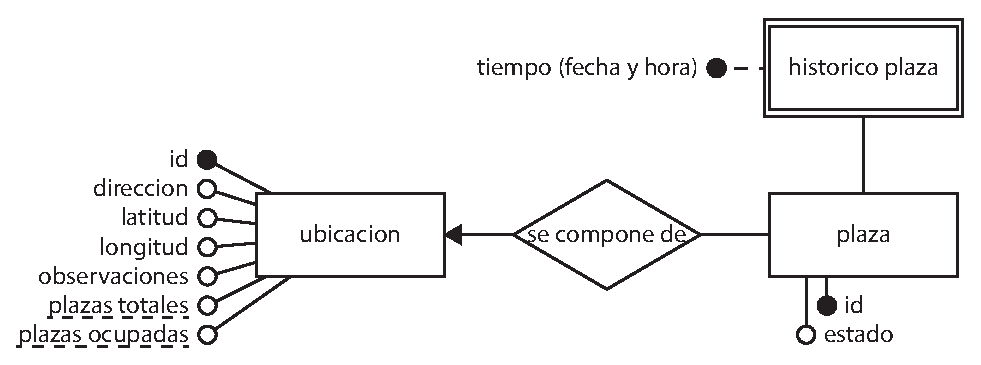
\includegraphics[width=0.7\textwidth]{imagenes/er_objetivo_4.eps}
	\caption{Esquema entidad-relación del objetivo 4}
	\label{er_objetivo_4}
\end{figure}
Por eficiencia del sistema y para saber cuántas de las plazas de una ubicación están ocupadas, se ha añadido un nuevo campo a las ubicaciones. Dicho campo se actualizará automáticamente según varíe el estado de las plazas de la ubicación.
\\\\
Una vez creadas las distintas tablas, en la API REST hay que crear los modelos para hacer un buen uso de estas tablas. Estos modelos tienen que tratar los datos en base a los casos de uso relacionados con el objetivo. Es por ello que, de momento, se tiene que dar de alta (añadir) plazas o ubicaciones, dar de baja (eliminar) plazas o ubicaciones y permitir modificar una ubicación existente. Además, se tendrá que visualizar la información contenida en el sistema, por lo que se debería sacar un listado de plazas y ubicaciones.
\\\\
Dicha funcionalidades en la API REST se tienen que materializar para que se pueda crear en la aplicación de gestión la parte de administración de plazas. Estas funcionalidades se han materializado de la siguiente forma:
\begin{itemize}
	\item Para dar de alta plazas se ha abierto la URI \textit{/plaza/nueva} con el método POST que recibe un JSON con el campo \textit{id\_ubicación}.
	\item Para dar de alta ubicaciones se ha abierto la URI \textit{/ubicacion/nueva} con el método POST que recibe un JSON con los campos \textit{direccion}, \textit{latitud}, \textit{longitud} y \textit{observaciones}.
	\item Para dar de baja una plaza se ha abierto la URI \textit{/plaza/<id>} con el método DELETE donde \textit{<id>} es el identificador de la plaza a eliminar.
	\item Para dar de baja una ubicación se ha abierto la URI \textit{/ubicacion/<id>} con el método DELETE donde \textit{<id>} es el identificador de la ubicación a eliminar.
	\item Para modificar una ubicación se ha abierto la URI \textit{/ubicacion/<id>} con el método POST donde \textit{<id>} es el identificador de la ubicación a modificar y recibe un JSON con los campos \textit{direccion} y \textit{observaciones}.
\end{itemize}
Todas estas funcionalidades devuelven un objeto JSON con un campo \textit{estado} que toma un valor booleano indicando si se ha podido realizar la operación. Al dar de alta una plaza, su estado es ``no definido'' y se actualiza el número de plazas totales de la ubicación donde se crea la plaza. De igual manera, cuando se elimina, se disminuye el número de plazas totales de la ubicación.
\\\\
De forma parecida, cuando se da de alta una ubicación, tanto el número de plazas totales como el de plazas ocupadas es cero. Y para eliminar una, estos dos campos deben estar a cero, es decir, que se hayan eliminado las plazas pertenecientes a la ubicación a eliminar.
\\\\
Para listar plazas y ubicaciones, las URIs son:
\begin{itemize}
	\item \textit{/plazas}, con método GET, que devuelve un objeto JSON con los campos \textit{num\_plazas} y \textit{plazas} que es una lista de objetos con los campos \textit{id}, \textit{estado} e \textit{id\_ubicacion}. 
	\item \textit{/ubicaciones} que devuelve un objeto JSON con los campos \textit{num\_ubicaciones} y \textit{ubicaciones}, con método GET, que es una lista de objetos con los campos \textit{id}, \textit{direccion}, \textit{latitud}, \textit{longitud}, \textit{plazas\_totales}, \textit{plazas\_ocupadas} y \textit{observaciones}. 
\end{itemize}
A las ubicaciones se le ha añadido un campo más en la tabla para saber qué número de sus plazas se encuentran ocupadas, \textit{plazas\_ocupadas}. Esta información va a ser útil de cara al usuario final de la aplicación móvil.
\\\\
Una vez que se encuentran hechas las funcionalidades en la API REST, en la aplicación de gestión hay que crear dos secciones: una que se encargue de la administración de las plazas y otra haga lo propio sobre las ubicaciones. Por supuesto, ambas páginas se actualizaran periódicamente para mostrar al administrador la ocupación real de las plazas que también se puede ver reflejada en las ubicaciones.
\\\\
También, los formularios para añadir plazas o ubicaciones, así como para modificar una ubicación, han sido validados tanto en el lado del cliente como en el lado de la API REST.
\\\\
Por otro lado, para facilitar la administración de las ubicaciones, se ha optado por incluir un mapa tanto en el listado de las ubicaciones como en la creación y modificación de la ubicación. Este mapa ha sido posible incluirlo a través de la API de Google \textit{Maps JavaScipt API} \cite{google-maps-js-api}.

\section{OBJ-5}
De igual manera que se ha hecho en el OBJ-4 se va a proceder en la implementación de éste. Lo primero es mirar en la matriz de trazabilidad, figura \ref{trazOBJ-R}, con qué requisitos de información y casos de uso está relacionado. Podemos ver que el OBJ-5 está relacionado con el requisito de información IRQ-3 y los casos de uso UC-7 y UC-8.
\\\\
Al igual que se ha hecho anteriormente, se debe hacer un esquema entidad-relación con la información que brinda el IRQ-3. Este esquema es el que se puede ver en la figura \ref{er_objetivo_5}.
\begin{figure}[H]
	\centering
	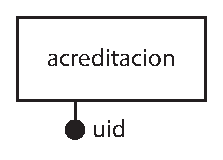
\includegraphics[width=0.15\textwidth]{imagenes/er_objetivo_5.eps}
	\caption{Esquema entidad-relación del objetivo 5}
	\label{er_objetivo_5}
\end{figure}
Como se puede observar, por ahora, sólo se guarda el identificador de la acreditación en el sistema. Esto hace que el sistema en sí no contenga datos de carácter personal ni información disgregada, ya que con esta información se podría llegar a saber la identidad de una persona.
\\\\
Este identificador (UID) es el identificador de la tarjeta pasiva RFID según el estándar ISO/IEC 15693 \cite{rfid-uid}. Dicho campo es de sólo lectura y único. También se puede ver el formato y la longitud de este identificador, que va a servir para verificar que el vehículo que ocupe una plaza monitorizada tiene autorización para ello.
\\\\
Una vez creada la tabla en la base de datos, así como su modelo y controlador en la API REST, las URIs que ésta tiene públicas para la administración de acreditaciones son:
\begin{itemize}
	\item \textit{/acreditaciones}, con método GET, que devuelve JSON con los campos \textit{num\_acreditaciones} y \textit{acreditaciones} que es un listado de las mismas. Dichas acreditaciones sólo tienen un campo que es \textit{uid}.
	\item \textit{/acreditacion/nueva}, con método POST, que recibe un JSON con el campo \textit{uid} y devuelve si se ha creado correctamente la nueva acreditación en el sistema.
	\item \textit{/acreditacion/<uid>}, con método DELETE, donde \textit{<uid>} es el UID de la tarjeta RFID que se quiere eliminar del sistema.
\end{itemize}
Una vez que se han publicado las URIs en la API REST, hacer la página de gestión de acreditaciones en la aplicación web de gestión no es tarea especialmente compleja. Además, y para evitar sobrecargas innecesarias, esta información no necesita actualizarse de forma periódica puesto que, para cambiar dicha información, el administrador necesita realizar acciones en dicha página.

\section{OBJ-6}
Esta parte del proyecto es vital debido a que el sistema tiene que tener información verídica del estado de ocupación de las plazas de aparcamiento. Para ello se va a proceder a crear un prototipo de agente de captación con sensores que actualice en tiempo real la información del sistema.
\\\\
Para ello, la primera decisión que hay que tomar es qué microcontrolador elegir. Tal y como se ha expuesto en el análisis, sección \ref{requisito-hw}, este microcontrolador debería disponer de WiFi para poder conectarse de manera inmediata con la API REST.
\\\\
El microcontrolador con WiFi que actualmente está revolucionando el mundo IoT (Internet of things, Internet de las cosas) a nivel doméstico, al estar presente en la electrónica de casi todos los dispositivos ``inteligentes'', es el ESP8266 \cite{esp8266}. Éste se puede encontrar en multitud de placas de desarrollo, entre ellas NodeMCU \cite{nodemcu}, Adafruit Huzzah \cite{huzzah}, SparkFun \cite{sparkfun-esp8266} o Wemos. Tanto Adafruit como SparkFun son dos de las grandes empresas de componentes de electrónica a nivel mundial que también tienen implicación por enseñar la llamada cultura \textit{maker}.
\\\\
Principalmente por motivo presupuestario pero sin obviar su funcionalidad, para este prototipo se ha optado por elegir la placa \textit{D1 mini Pro} de Wemos \cite{d1}. Esta placa presenta WiFi integrado, 11 pines de los cuales uno de ellos es analógico y dos de ellos son de trasmisión de datos y tres pines de alimentación (tierra, 5V y 3.3V).
\\\\
Una vez que ya está elegida la placa de desarrollo, el paso siguiente es ver cómo se puede programar. Este microcontrolador tiene la capacidad de poderse programar en NodeMCU \cite{nodemcu-firmware} (proveniente de Lua \cite{lua}), MicroPython \cite{micropython} o Arduino \cite{arduino}. Dado que NodeMCU y MicroPython son ambos lenguajes interpretados, se ha optado por programar al microcontrolador en Arduino.
\\\\
En NodeMCU y MicroPython lo que se hace es re-programar la memoria del microcontrolador con un intérprete que va leyendo el programa de la memoria y actúa en consecuencia. Esto hace que la velocidad de ejecución disminuya además de los problemas de seguridad relacionados al tener el código fuente en la memoria de la placa.
\\\\
Ahora que se sabe qué placa de desarrollo utilizar y cómo programarla, es el momento de buscar los sensores necesarios para la creación del prototipo. Para ello se va a elegir un receptor RFID para leer la credencial del usuario, si dispone, y un sensor de ultrasonidos para detectar al vehículo. 
\\\\
Con respecto al receptor RFID, se va a empezar por un dispositivo pequeño que sirva de ilustración en este prototipo. El receptor que más se utiliza es el MFRC522 \cite{rfid-especs}. Existen numerosas placas ya montadas para la creación de prototipos con este receptor. Una de ellas, y la más común, es RFID-RC522 \cite{rfid-modulo}.
\\\\
Dicho módulo se comunica con el microcontrolador a través de un BUS SPI que es un BUS síncrono, full dúplex con cuatro líneas \cite{spi}. Dichas lineas son:
\begin{itemize}
	\item SCK: línea de reloj.
	\item MOSI: línea de trasmisión maestro-esclavo.
	\item MISO: línea de trasmisión esclavo-maestro.
	\item SS: línea de selección del esclavo.
\end{itemize}
Realmente el microcontrolador ESP8266 soporta tan solo un dispositivo conectado a este BUS de acorde con su documentación \cite{esp8266-pins}.
\\\\
Siguiendo con la elección de los dispositivos hardware y antes de entrar a programar el agente de captación de datos, falta por seleccionar el sensor de ultrasonidos. Se puede ver en una búsqueda rápida que el más usado para la creación de prototipos es el HC-SR04 \cite{hcsr04}.
\\\\
El funcionamiento por el cual este sensor calcula la distancia entre él y un objeto es midiendo el tiempo de rebote de una onda sonora. Como se sabe que la velocidad del sonido en condiciones óptimas en la atmósfera terrestre es de $343m/s$, se puede calcular la distancia despejando la ecuación del movimiento rectilíneo uniforme: $$Distancia = Tiempo \times Velocidad$$ Dicha distancia sería la recorrida por el sonido desde que sale del sensor, rebota en el objeto y llega al sensor, por lo que la distancia entre el sensor y el objeto sería la mitad.
\\\\
Una vez que están los componentes del agente de captación de datos, el siguiente paso es proceder al montaje de dichos componentes:
\begin{itemize}
	\item RFID-RC522:
	\begin{itemize}
		\item 3.3V - Wemos 3.3V
		\item RST  - Wemos D3
		\item GND  - Wemos GND
		\item IRQ
		\item MISO - Wemos D6
		\item MOSI - Wemos D7
		\item SCK  - Wemos D5
		\item SDA  - Wemos D8
	\end{itemize}
	\item HC-SR04:
	\begin{itemize}
		\item VCC  - Wemos 5V
		\item Trig - Wemos D1
		\item Echo - Wemos D2
		\item GND  - Wemos GND
	\end{itemize}
	\item LED verde: Wemos RX - GND
	\item LED rojo: Wemos TX - GND
\end{itemize}
\begin{figure}[H]
	\centering
	\includegraphics[width=\textwidth]{imagenes/esquema_agente_captacion.pdf}
	\caption{Vista montaje agente de captación de datos}
	\label{esquema-agente-captacion}
\end{figure}
Como se puede ver, se han añadido dos LEDs, uno rojo y otro verde, que sirven para saber cuál es el estado de la plaza. Si el verde queda fijo, la plaza se encuentra bien ocupada. En cambio, si el rojo se queda fijo, la plaza está mal ocupada. Cuando ambos están apagados significa que la plaza está libre y si se encuentran parpadeando alternativamente es que se ha producido algún tipo de fallo en la comunicación con el servidor.
\\\\
Antes de entrar a programar el microcontrolador es necesario añadir dos URIs en la API REST:
\begin{itemize}
	\item \textit{/plaza/<id>/estado/<nuevo\_estado>}, con método PUT, donde \textit{<id>} es el identificador de la plaza de aparcamiento que se quiere cambiar el estado y \textit{<nuevo\_estado>} es el estado al que ha cambiado la plaza. Se devuelve un JSON con el identificador de la plaza y un booleano que indica si se ha actualizado correctamente.
	\item \textit{/acreditacion/<uid>}, con método GET, donde \textit{<uid>} es el UID de una tarjeta que se quiere comprobar que existe en el sistema. Se devuelve un JSON con el campo \textit{estado} a \textit{True} si existe y un error 404 en caso contrario.
\end{itemize}
La funcionalidad de la segunda es trivial. Sin embargo, la de la primera, no tanto. Ésta tiene que comprobar que el identificador de la plaza exista en el sistema y el nuevo estado sea distinto al del anterior para evitar posibles paquetes perdidos. Una vez que pase dichas comprobaciones tendrá, por una parte que actualizar, si procede, las plazas ocupadas de la ubicación donde se encuentra la plaza. Por otra parte tendrá que añadir en el histórico que se ha producido un cambio de estado en la plaza. Y, finalmente, actualizar el estado de la plaza en su tabla.
\\\\
\newpage
Una vez que se han añadido las dos URIs con su funcionalidad correspondiente a la API REST, se puede proceder a la programación del microcontrolador con Arduino, un lenguaje parecido a C, al cual se le puede añadir funcionalidades haciendo librerías en C/C++.
\\\\
Por suerte, Arduino ya tiene implementadas bastantes librerías. Una de ellas es SPI para poder usar el lector RFID. Además de las propias, hay contribuciones externas como es el caso de la librería ESP8266, para usar este microcontrolador en Arduino; MFRC522, para usar el lector RFID; o ArduinoJson para trabajar con objetos JSON.
\\\\
Aunque haya muchas funcionalidades hechas, programar un microcontrolador, no es tarea fácil debido a que, sólo tiene una hebra de ejecución. Por este motivo, se tiene que hacer de manera óptima para que parezca que es capaz de ejecutar varias tareas a la vez. Estas tareas van a ser: leer la distancia del sensor de ultrasonidos, leer el UID de la tarjeta cuando el sensor de ultrasonidos detecte un vehículo y el aparcamiento no esté actualizado, comprobar enviando una petición al servidor si la acreditación leída existe y actualizar el estado enviando otra petición al servidor en consecuencia con lo anterior.
\\\\
Como no va a estar constantemente midiendo la distancia, se ha programado una interrupción de reloj, cada cinco segundos, para proceder a esta acción. El único proceso donde el microcontrolador tiene que realizar una espera activa, y por tanto se nota que no funciona en tiempo real, es cuando se conecta con el servidor para hacer peticiones.
\\\\
En el lector RFID se podría colocar una línea de interrupción (pin IRQ) para que avise al microcontrolador en el momento de leer una tarjeta. Esta interrupción se ha optado por no hacerla debido a que, para leer la tarjeta, se tiene que hacer una petición expresa para ver si está detectándola.
\\\\
Por último, hay que establecer una distancia de detección, esto es, el módulo HC-SR04 va a medir la distancia hasta el primer objeto que se encuentre en un rango de 2cm a 4 metros. Si el objeto se encuentra más alejado de la distancia de detección, la plaza de aparcamiento estaría libre. En cambio, si éste se encuentra más cerca de la distancia de detección se infiere que hay un vehículo ocupando la plaza. También, se podría establecer un valor mínimo y así comprobar que el objeto se encuentra en un rango, por ejemplo la altura de los bajos de un vehículo.
\\\\
Con todo esto y una vez hecho el programa, se procede a programar el microcontrolador y a comprobar que funcione correctamente tanto la detección, a través de los sensores, como la conexión a la API REST. Con esto, el siguiente paso es modificar la aplicación de gestión para recibir alertas.

\section{OBJ-3}
Una vez que el agente de captación está creado y se han programado las distintas funcionalidades en la API REST, se va a proceder a crear un script, en la aplicación de gestión, para recibir alertas cuando alguna plaza esté mal ocupada. Pero antes de eso, hay que crear la funcionalidad en el servidor.
\\\\
Como en la tabla \textit{histórico plaza} se va guardando el estado de una plaza junto con la marca de tiempo cuando cambia, hay que ver aquí qué plazas están mal ocupadas para así sacar desde cuándo están mal ocupadas. La consulta para ello sería compuesta sacando el último estado de las plazas en esta tabla. Para ello se tiene que usar la cláusula \textit{distinct} en el identificador de la plaza. Después de esta primera consulta, la siguiente sería seleccionar aquellas tuplas cuyo estado sea \textit{mal ocupada}.
\\\\
Una vez que se ha creado la funcionalidad en el servidor y abierta la URI,\\
\textit{/plazas/mal\_ocupadas}, con método GET, que devuelve un JSON con el listado de plazas junto a la marca de tiempo de ocupación y cuyo estado es \textit{mal ocupada}, se puede proceder a sacar alertas en la aplicación.
\\\\
Para este último paso, se ha decidido usar una librería de muestra de notificaciones usando Bootstrap, Bootstrap Notify \cite{bootstrap-notify} bajo licencia MIT. Éstas mostrarán un mensaje en la parte superior derecha de la pantalla con aquellos identificadores de plazas junto a la hora y fecha del momento en el cual han sido mal ocupadas. Al pinchar en dicha notificación, la aplicación mostrará la página de administración de plazas.
\\\\
Estas notificaciones, al igual que la información de las plazas, se actualiza cada 10 segundos que es un intervalo de tiempo razonadamente corto y evita sobrecargar el servidor.

\section{OBJ-7}
Una vez que el sistema está funcionando y se puede administrar, el último paso de este proyecto es la creación de una aplicación móvil para el usuario final. Antes y hacer el caso de uso procedente, UC-10, hay que elegir con qué tecnología se va a crear dicha aplicación.
\\\\
A día de hoy existen diversos frameworks de desarrollo que permiten hacer una aplicación móvil multiplataforma, esto es, un único desarrollo daría como resultado varias aplicaciones: una para Android, otra para IOS y otra para Windows Phone. También se pueden hacer aplicaciones llamada Web-APPS con Ionic \cite{ionic} o con PhoneGap \cite{phonegap} entre otros muchos frameworks de desarrollo de ese estilo que hacen una aplicación a través de usar tecnología web.
\\\\
En ambos casos lo que realmente se está haciendo es \textit{transpilar}, es decir, generar un lenguaje a partir de otro para así hacer una aplicación. Aunque el desarrollo, en muchos casos, es más rápido y multiplataforma, la aplicación definitiva es más ineficiente que una desarrollada a mano. Por otro lado, tras actualizaciones en las plataformas de desarrollo (Android o IOS) hay muchos problemas al hacer una aplicación que necesite algún componente específico que es el caso de la aplicación que aquí se va a hacer. 
\\\\
Esto se dice porque, en primera instancia para desarrollar la aplicación móvil, se optó por Xamarin. Éste es un framework para desarrollar aplicaciones móvil multiplataforma propiedad de Microsoft. El desarrollo fue fácil al tener experiencia en C\# pero en el momento de necesitar componentes específicos como un mapa para poder las ubicaciones de aparcamiento en la aplicación, el desarrollo quedó estancado debido a que el gestor de paquetes de Xamarin no podía resolver las dependencias de algunos de ellos tras la actualización de la API de Google Maps. Dicha incidencia supuso un atraso en el desarrollo.
\\\\
Tras la mala experiencia, se decidió cambiar de mentalidad y desarrollar la aplicación de forma nativa para una sola plataforma: Android.
\\\\
Nada más comenzar a crear el proyecto en Android Studio para hacer la aplicación, después de elegir la plataforma base para el proyecto, hay que elegir un \textit{Activity} base. En dichos \textit{Activities}, por defecto hay una donde muestra un mapa de Google Maps.
\\\\
Lo primero que se tendría que hacer es mostrar en dicho mapa las ubicaciones de aparcamiento. Este listado de ubicaciones puede ser el mismo que se hizo para la aplicación pero, de esta manera sería ineficiente y presentaría un gasto de transmisión muy grande actualizar la información de la aplicación.
\\\\
Para resolver este problema y al sólo necesitar los datos de aquellas ubicaciones localizadas dentro de una zona determinada, ventana de visualización del mapa, se puede hacer diferentes peticiones dependiendo de la zona que se muestre en la aplicación. Por este motivo es necesario añadir una nueva URI con esta funcionalidad a la API REST.
\\\\
Esta nueva URI es:
\\
\textit{/ubicaciones/<lat\_min>\&<lat\_max>/<long\_min>\&<long\_max>}, con método GET, donde \textit{lat\_min} y \textit{long\_min} es la latitud y longitud de la esquina superior derecha y \textit{lat\_max} y \textit{long\_max} es lo propio de la esquina inferior izquierda de la zona visible de un mapa. Este método devuelve una un JSON con el número de ubicaciones incluidas en esa zona y un listado de ellas.
\\\\
Con esta nueva funcionalidad en la API REST, la aplicación móvil puede hacer una petición al servidor al detectar que se ha movido, ampliado o alejado el mapa, es decir, cuando ha habido algún tipo de cambio en la visualización del mismo. Para la conexión con el servidor se ha optado por usar, la librería de Android, Volley \cite{volley}.
\\\\
Una vez que se tiene los datos en la aplicación móvil, se tienen que visualizar. Para ello se tiene que usar la API de desarrollo de Google \cite{android-maps}. Antes de continuar, para poder hacer todo esto y poder visualizar correctamente el mapa en la aplicación, se debe obtener una \textit{API key} y activarla en la cuenta de desarrollador de Google.
\\\\
Ahora que se puede visualizar correctamente el mapa con las ubicaciones de aparcamiento, se procede a la creación de dos nuevos \textit{Activities}. El primero se va a mostrar cuando el usuario seleccione una ubicación del mapa. En este caso se le mostrará una pantalla con los datos actualizados de dicha ubicación y un botón para navegar hasta ella. El segundo se activará cuando el usuario marque otra posición distinta en el mapa. Este caso es el OBJ-8.
\\\\
Antes de proceder con él, hay que saber cómo navegar hasta la ubicación deseada. Para ello, lo que se ha pensado es hacer uso de la navegación de la aplicación Google Maps, que viene instalada en Android por defecto. Para ello se deben usar los \textit{intents} de Google Maps \cite{android-maps-intent}.
\\\\
Por último, se debería informar al usuario cuando se encuentra navegando a una ubicación si dicha ubicación se queda sin plazas disponibles. Para esto, la única solución es usando un servicio de notificaciones.
\\\\
Google también lo tiene solucionado con su servicio \textit{Cloud Messaging} ahora en Firebase \cite{firebase}. Este servicio se integra perfectamente con Android y, por parte del servidor, tiene SDK para python -\textit{firebase-admin}-.
\\\\
Pero para mandar la notificación se necesita saber a quién y cuándo mandarla. En respuesta a cuándo se mandaría sería en el momento que se actualice el estado de una plaza, en el caso de que la plaza quedase ocupada y fuese la última en esa ubicación. Para dar respuesta al quién, se necesita guardar en el servidor el destino del usuario junto al token que se usa en Firebase para mandar notificaciones a usuarios. Dicho token es único por dispositivo, es decir, un identificador.
\\\\
Es por ello que esta meta de desarrollo está relacionada con el requisito de información IRQ-6. Esta nueva información encajaría de la siguiente manera en la base de datos:
\begin{figure}[H]
	\centering
	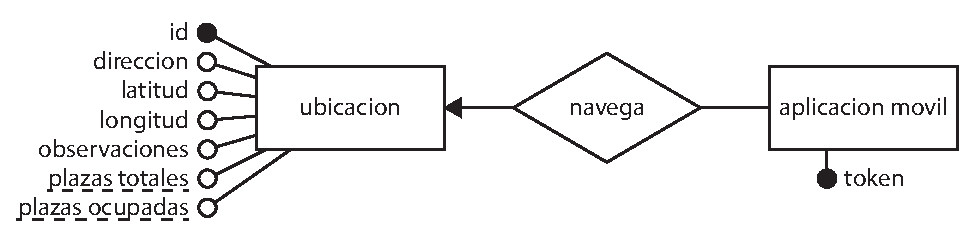
\includegraphics[width=0.7\textwidth]{imagenes/er_objetivo_7.eps}
	\caption{Esquema entidad-relación del objetivo 7}
	\label{er_objetivo_7}
\end{figure}
Una vez creada la tabla, hay que hacer su modelo y controlador en la API REST. Dicho controlador tendría las siguientes URIs abiertas:
\begin{itemize}
	\item \textit{/destino\_activo/nueva}, con método POST, que recibe un JSON con los campos \textit{id\_ubicacion} que es el identificador de ubicación donde el usuario se dispone a ir y \textit{token} que es el identificador del dispositivo del usuario. Esta funcionalidad da de alta un destino activo en el sistema.
	\item \textit{/destino\_activo/<token>}, con método DELETE, donde \textit{<token>} es el identificador del dispositivo del usuario para eliminarlo del sistema de notificaciones.
\end{itemize}
Estas dos funcionalidades devuelven un objeto JSON para afirmar si la operación se ha realizado correctamente. A la primera URI la aplicación móvil la llamaría justo antes de crear el intent de Google Maps para navegar. A la segunda, se llamaría al volver de Google Maps a la aplicación o al volver a abrir la aplicación.

\section{OBJ-8}
Para que la aplicación sea más útil, se ha pensado en que muestre una lista de ubicaciones cuando el usuario selecciona un destino en el municipio. A partir de ese destino, el sistema deberá escoger las mejores ubicaciones de aparcamiento para el usuario.
\\\\
Antes de explicar cómo se filtran las ubicaciones que se muestran en la lista, se puede observar en la matriz de trazabilidad, figura \ref{trazOBJ-R}, que este objetivo está relacionado con el requisito de información IRQ-5. Esto se debe a que se quiere recoger datos para un posterior estudio de la localización de las plazas en base al destino real de los usuarios que las usan. Estos datos se recogen de forma anónima en la siguiente tabla, sacada a partir de las especificaciones del requisito de información IRQ-5:
\begin{figure}[H]
	\centering
	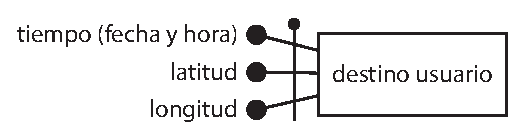
\includegraphics[width=0.4\textwidth]{imagenes/er_objetivo_8.eps}
	\caption{Esquema entidad-relación del objetivo 8}
	\label{er_objetivo_8}
\end{figure}
Esta tabla se va rellenando con los diferentes destinos de los usuarios cuando éstos hacen búsquedas en la aplicación. Pero para que se pueda hacer esto, es necesario crear la funcionalidad en la API REST que reciba las coordenadas de destino del usuario y le devuelva una lista de ubicaciones donde poder aparcar. Esta URI sería: \textit{/destinos\_usuario/nueva<lat>\&<long>}, con método PUT, siendo \textit{<lat>} y \textit{<long>} la latitud y longitud, respectivamente, del destino del usuario.
\\\\
\newpage
Por otro lado, la pantalla de la aplicación móvil que muestra un listado de ubicaciones dado el destino del usuario también necesita de una funcionalidad en la API REST para obtener dicho listado. Estas URI serían:
\begin{itemize}
	\item \textit{/ubicaciones/<lat>\&<long>}, con método GET, siendo \textit{<lat>} y \textit{<long>} la latitud y longitud, respectivamente, del destino del usuario.
	\item \textit{/ubicaciones/<lat>\&<long>/<grano>}, con método GET, siendo \textit{<lat>} y \textit{<long>} la latitud y longitud, respectivamente, del destino del usuario y \textit{<grano>} una distancia en metros para agrupar ubicaciones.
\end{itemize}
Ambas URIs devuelven una lista ordenada de ubicaciones.
\\\\
En la primera, el parámetro \textit{grano} se define a 0. Este parámetro ayuda a reordenar las ubicaciones. En principio, cuando el parámetro es 0, las ubicaciones se ordenan por distancia al destino marcado por el usuario. El parámetro lo que hace es crear grupos de ubicación que estén en el mismo rango de distancia con respecto al destino. Dentro de estos grupo las ubicaciones se ordenan por número de plazas disponibles. 
\\\\
Esto da lugar a que, si el valor del parámetro incrementa, aquellas ubicaciones que se encuentren más lejos del destino pero que tengan un mayor número de plazas libres, van a ir apareciendo en primeras posiciones. Es elección del usuario darle valor a dicho parámetro teniendo en cuenta cuánto se quiere desplazar.
\\\\
Para afinar el filtrado de las ubicaciones se ha pensado en utilizar un histórico de ocupación de las ubicaciones en base al histórico de ocupación de las plazas. Con esta información se podría elaborar un porcentaje de ocupación de una determinada zona en el tiempo.
\\\\
Por tanto, como las personas en general tenemos patrones de comportamiento, con el porcentaje anteriormente detallado se puede hacer una predicción del estado de ocupación de una ubicación en el futuro. Esto serviría para decirle al usuario cómo estará la ubicación cuando vaya a aparcar o serviría para que el sistema dirija al usuario a la ubicación donde tiene más probabilidades para estacionar, en base al tiempo que tardaría en llegar al lugar.
\\\\
Pero no todo hay que basarlo en el histórico, sino que, a su vez, datos como la climatología o los eventos de una ciudad, pueden estar relacionados con la ocupación de estos aparcamientos. Es por esto que el sistema va a quedar preparado para adaptar esta información para afinar la lista de ubicaciones que se le brinda al cliente.
\\\\
Puesto que para hacer esto se necesitarían bastantes datos, se pensó en la creación de un generador de datos que se comporte de manera esperada a como lo harían los usuarios de este tipo de aparcamientos. Este generador sería lo suficientemente complejo para suponer otro TFG, por lo que queda para un trabajo futuro junto con la integración de un agente con una base de conocimiento mayor que prediga la ocupación de la ubicación en el futuro.
\newpage
\chapter{Manual de usuario}
Como se ha podido ver en la descripción de la solución propuesta y en su implementación, se han creado dos aplicaciones de cara al usuario: una aplicación de administración y una aplicación móvil para el usuario final. En esta sección se va a realizar un recorrido por estas dos aplicaciones explicando al usuario cómo funcionan.
\section{Aplicación de administración}
La aplicación de administración está creada para que los usuarios provenientes de la Administración Pública y la autoridad puedan gestionar el sistema vía web. Esta gestión es: administrar las plazas de aparcamiento y las acreditaciones para aparcar en este tipo de plazas, así como recibir alertas de plazas que estén siendo mal usadas.
\\\\
En todas las pantallas de la aplicación aparecen notificaciones cuando un vehículo sin acreditación ocupa un aparcamiento. Estas notificaciones se actualizan cada 15 segundos y al pulsar sobre ellas van a dirigir al usuario a la pantalla de gestión de plazas. A continuación se puede ver un ejemplo de estas notificaciones:
%\begin{figure}[H]
%	\centering
%	\includegraphics[width=0.9\textwidth]{imagenes/administracion/alerta.png}
%	\caption{Vista principal: ejemplo alerta plaza mal ocupada}
%	\label{administración_alerta}
%\end{figure}
%La pantalla que se muestra anteriormente es la principal de la aplicación donde el usuario puede acceder a las diversas secciones de la misma: gestión de plazas, ubicaciones o acreditaciones; como se puede ver en la figura \ref{administración_alerta}. Aquí el administrador puede elegir qué gestionar. 

\subsection{Gestión de ubicaciones de aparcamiento}
Si el administrador quiere gestionar las ubicaciones de aparcamiento del sistema, debería acceder a ``Ubicaciones''. Estas son donde existen las plazas de aparcamiento monitorizadas.
\begin{figure}[H]
	\centering
	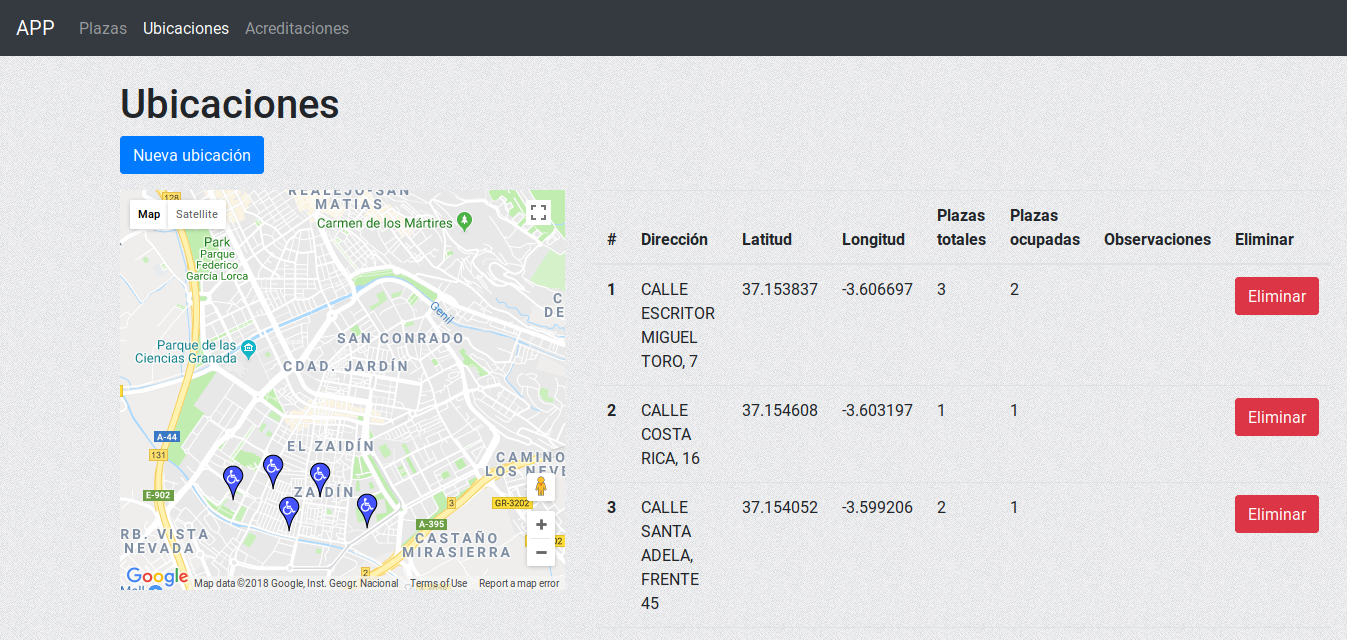
\includegraphics[width=0.9\textwidth]{imagenes/administracion/ubicaciones.png}
	\caption{Vista de ubicaciones: aplicación de administración}
	\label{administracion_ubicaciones}
\end{figure}
En esta sección, figura \ref{administracion_ubicaciones}, se pueden ver las distintas ubicaciones existentes en el sistema, ya sea posicionadas en el mapa o en la lista con más detalles como su dirección, coordenadas GPS, número de plazas u observaciones. Este pantalla se actualiza automáticamente para que su información sea en tiempo real ya que el número de plazas ocupadas podría cambiar. También da la posibilidad de añadir una nueva ubicación, figura \ref{administracion_ubicaciones_nueva}, donde hay que administrarle una posición GPS a mano o pinchando la posición en el mapa y una dirección. Las observaciones no son obligatorias.
\begin{figure}[H]
	\centering
	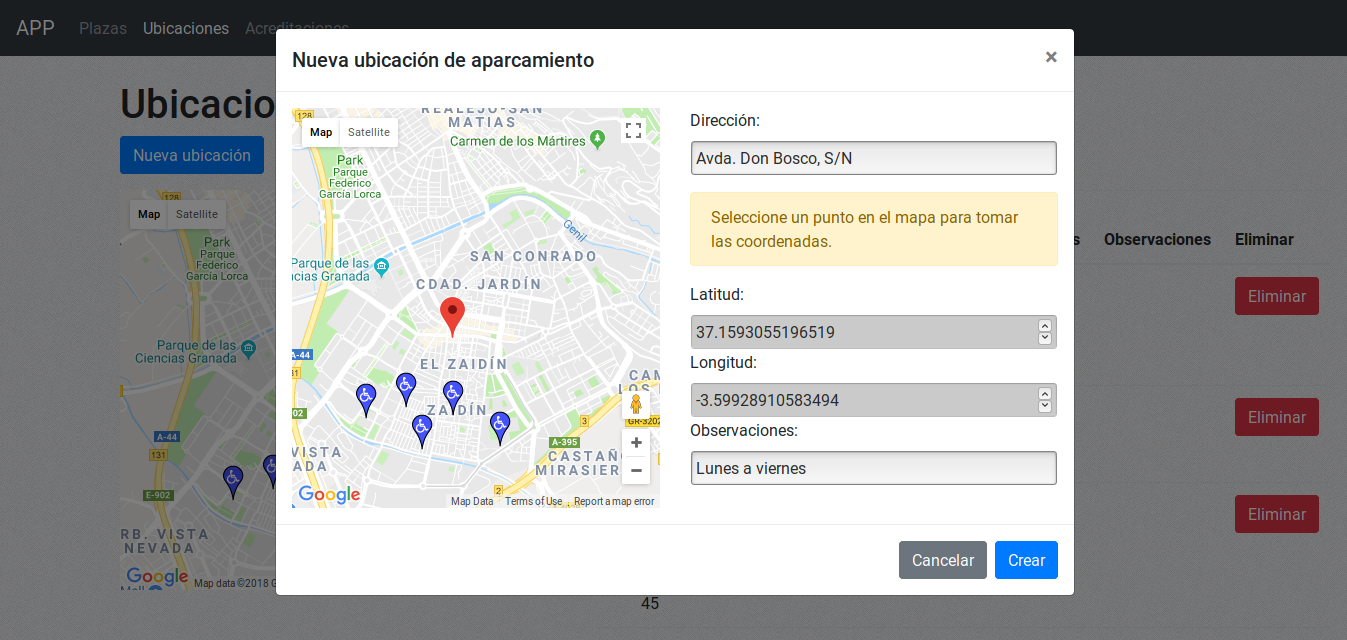
\includegraphics[width=0.9\textwidth]{imagenes/administracion/ubicaciones_nueva.png}
	\caption{Vista de creación de una nueva ubicación: aplicación de administración}
	\label{administracion_ubicaciones_nueva}
\end{figure}
Si no se indica ni la dirección ni las coordenadas de la ubicación, la aplicación advierte con un mensaje de error indicando que se necesita rellenar los datos obligatorios para dar de alta una nueva ubicación, figura \ref{administracion_ubicacion_nueva_error}.
\begin{figure}[H]
	\centering
	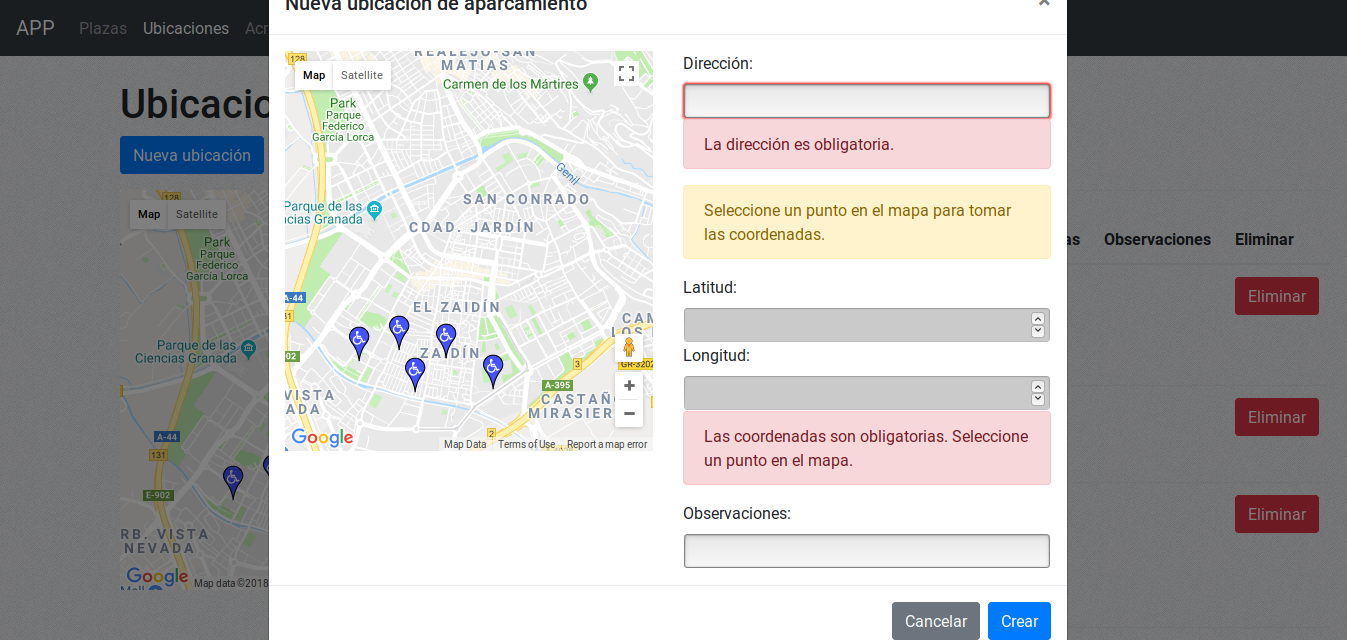
\includegraphics[width=0.9\textwidth]{imagenes/administracion/ubicaciones_nueva_error.png}
	\caption{Vista de error en la creación de una nueva ubicación: aplicación de administración}
	\label{administracion_ubicacion_nueva_error}
\end{figure}
Si se indican correctamente los datos para crear una nueva ubicación, el sistema añadirá la nueva ubicación, figura \ref{administracion_ubicaciones_creada}.
\begin{figure}[H]
	\centering
	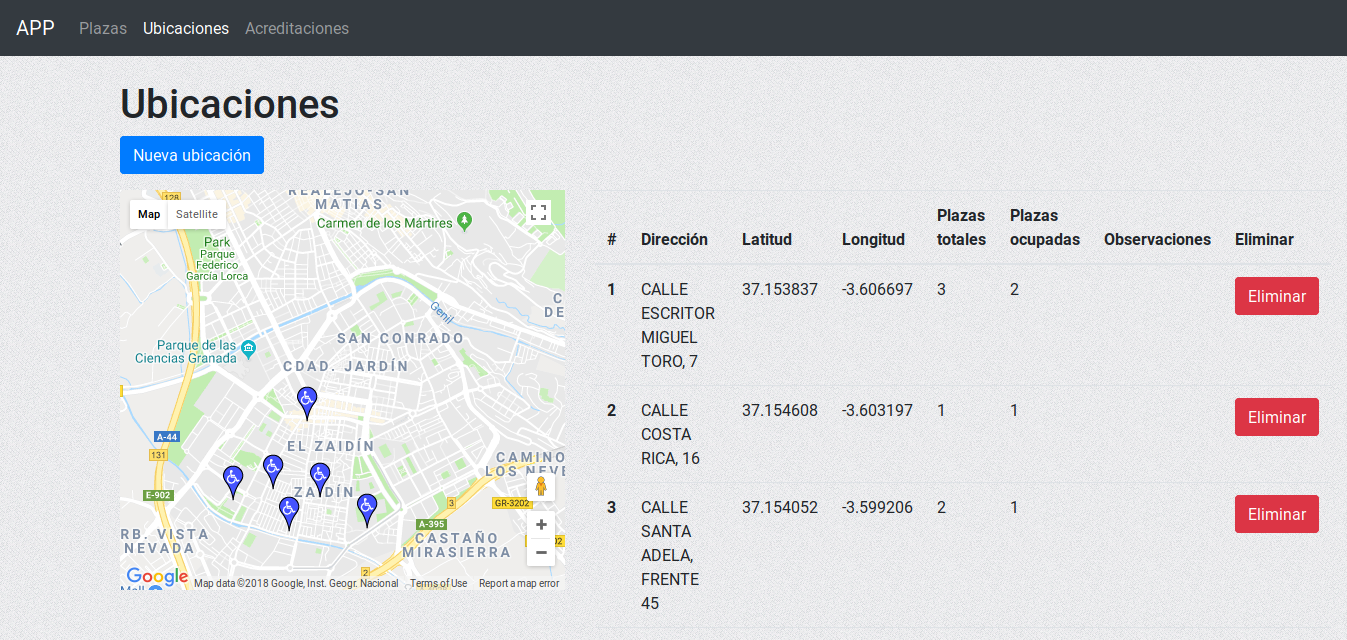
\includegraphics[width=0.9\textwidth]{imagenes/administracion/ubicaciones_creada.png}
	\caption{Vista listado con nueva ubicación: aplicación de administración}
	\label{administracion_ubicaciones_creada}
\end{figure}
En esta pantalla, junto al listado de las ubicaciones existentes, la aplicación permite eliminar de forma fácil una ubicación del sistema siempre y cuando no tenga plazas asociadas, figura \ref{administracion_ubicaciones_eliminar}.
\begin{figure}[H]
	\centering
	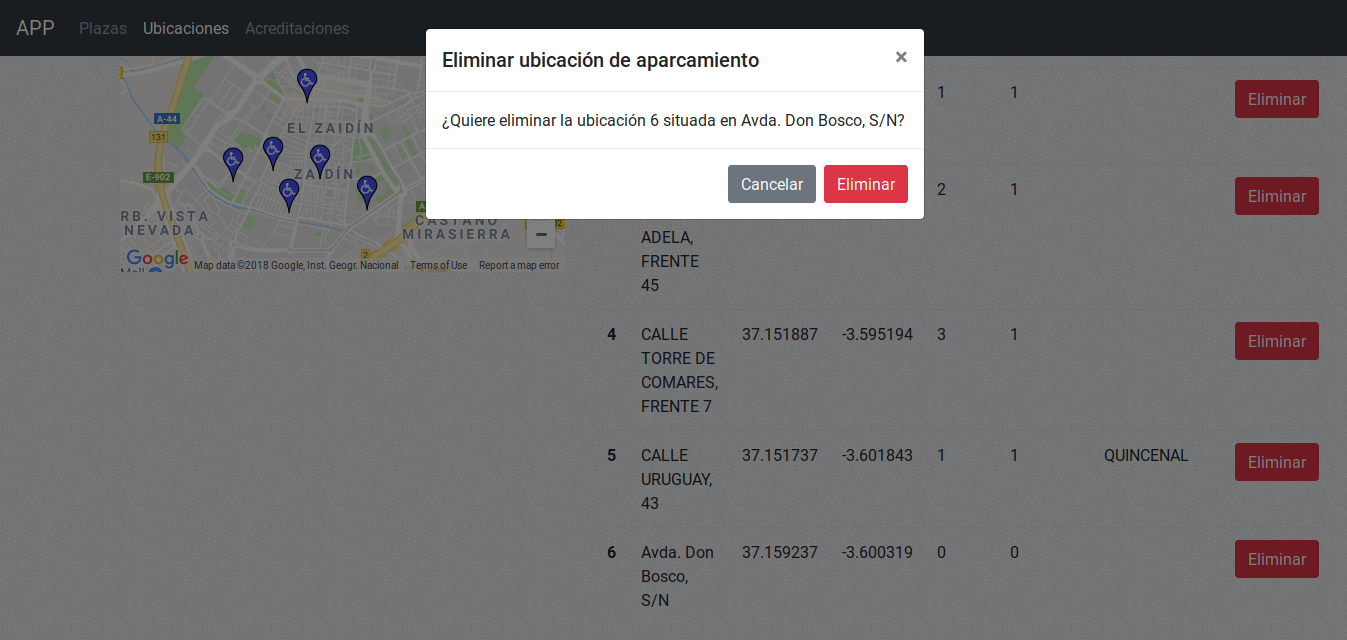
\includegraphics[width=0.9\textwidth]{imagenes/administracion/ubicaciones_eliminar.png}
	\caption{Vista de eliminación de una ubicación: aplicación de administración}
	\label{administracion_ubicaciones_eliminar}
\end{figure}
Si la ubicación que se quiere eliminar tiene plazas asociadas, no se podrá realizar la acción. Si se trata de eliminar, la aplicación muestra el siguiente mensaje de error:
\begin{figure}[H]
	\centering
	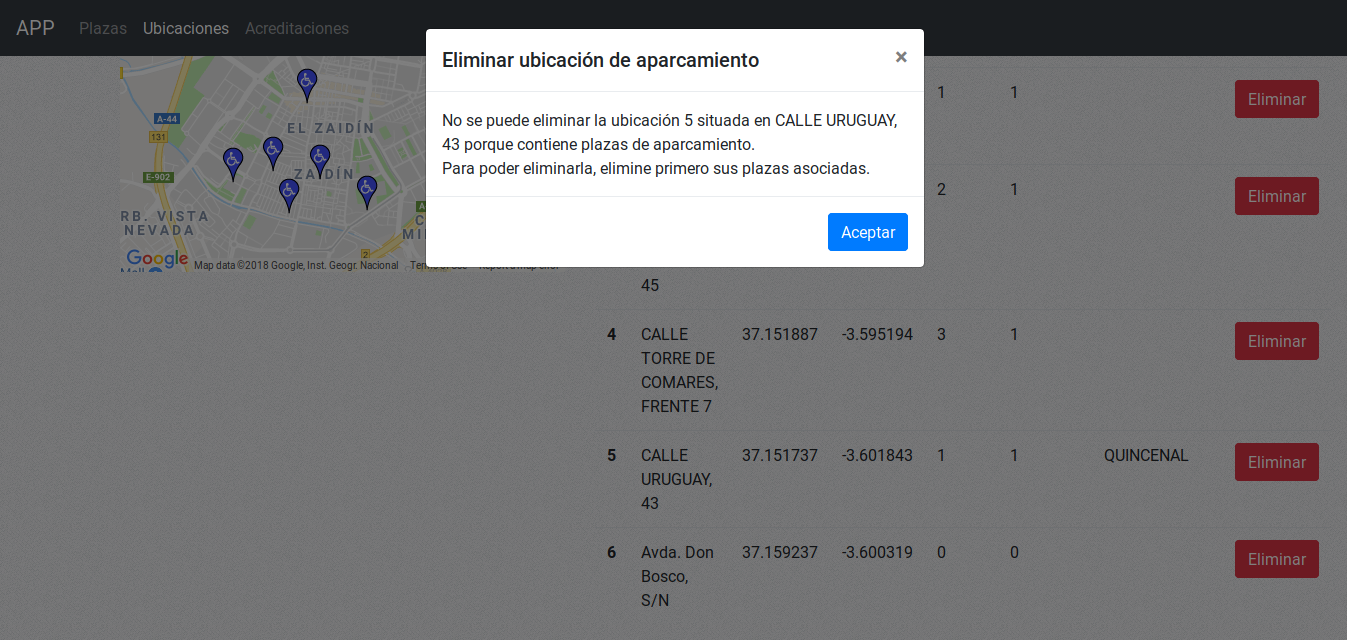
\includegraphics[width=0.9\textwidth]{imagenes/administracion/ubicaciones_eliminar_error.png}
	\caption{Vista de error en la eliminación de una ubicación: aplicación de administración}
	\label{administracion_ubicaciones_eliminar_error}
\end{figure}

\subsection{Gestión de plazas de aparcamiento}
Si el administrador quiere gestionar las plazas de aparcamiento del sistema, debería acceder a ``Plazas''. Estas son monitorizadas y tienen que estar en una ubicación a la que pertenece.
\begin{figure}[H]
	\centering
	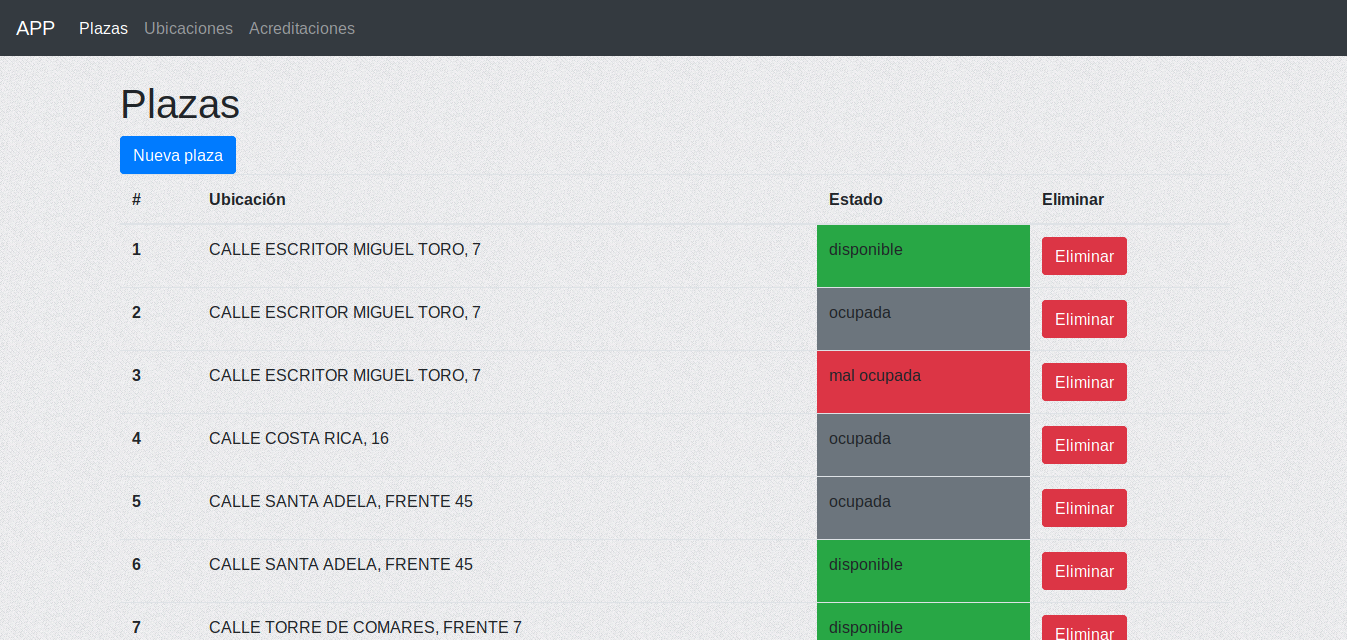
\includegraphics[width=0.9\textwidth]{imagenes/administracion/plazas.png}
	\caption{Vista de plazas: aplicación de administración}
	\label{administracion_plazas}
\end{figure}
En esta sección, figura \ref{administracion_plazas}, se pueden ver las distintas plazas existentes en el sistema junto a su estado actual: plaza disponible, ocupado o mal ocupado. Este pantalla se actualiza automáticamente para que su información sea en tiempo real. También da la posibilidad de añadir una nueva plaza, figura \ref{administracion_plazas_nueva}, donde hay que seleccionar aquella ubicación donde se quiere añadir la nueva plaza.
\begin{figure}[H]
	\centering
	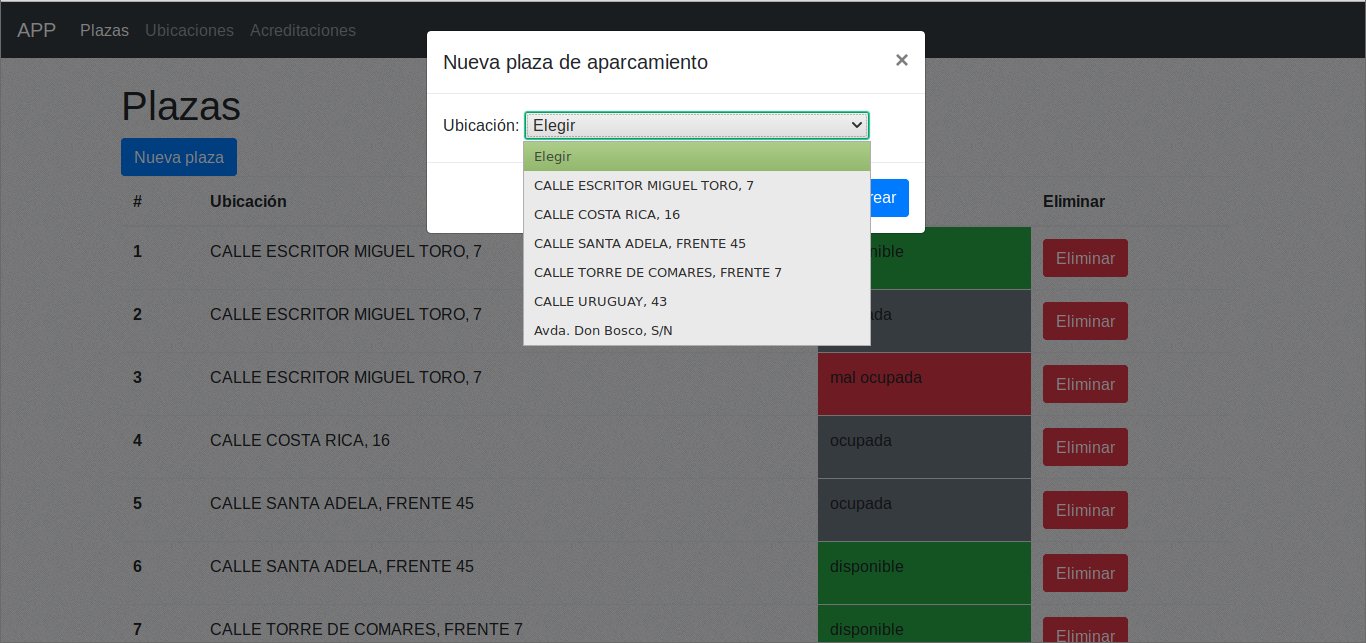
\includegraphics[width=0.9\textwidth]{imagenes/administracion/plazas_nueva.png}
	\caption{Vista de creación de una nueva plaza: aplicación de administración}
	\label{administracion_plazas_nueva}
\end{figure}
Si no se indica dicha ubicación, la aplicación advierte con un mensaje de error indicando que se necesita seleccionar una ubicación, figura \ref{administracion_plazas_nueva_error}.
\begin{figure}[H]
	\centering
	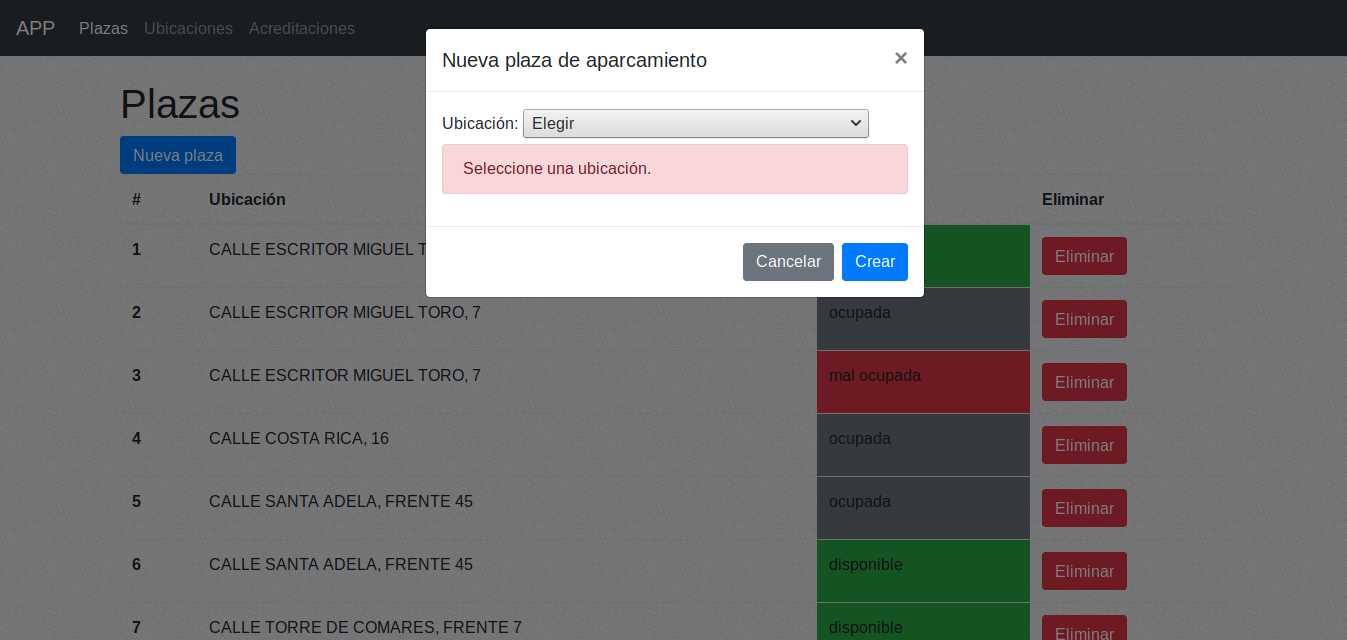
\includegraphics[width=0.9\textwidth]{imagenes/administracion/plazas_nueva_error.png}
	\caption{Vista de error en la creación de una nueva plaza: aplicación de administración}
	\label{administracion_plazas_nueva_error}
\end{figure}
Si se selecciona una ubicación, el sistema creará la nueva plaza, figura \ref{administracion_plazas_creada}.
\begin{figure}[H]
	\centering
	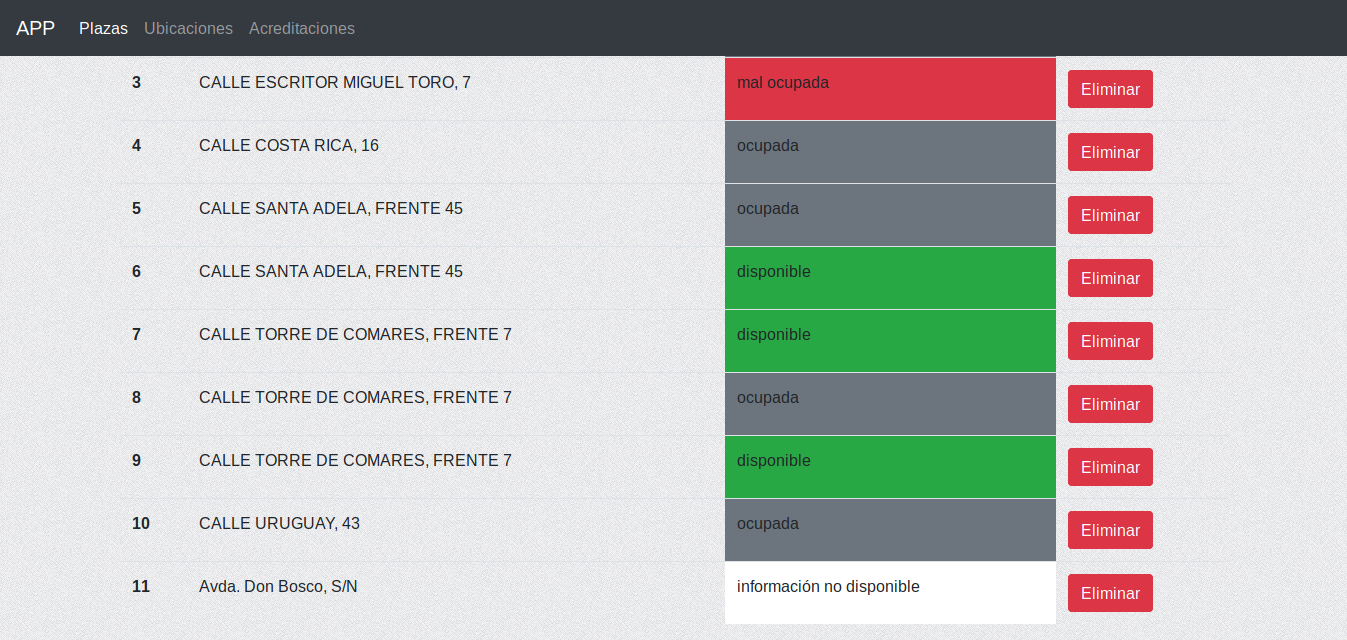
\includegraphics[width=0.9\textwidth]{imagenes/administracion/plazas_creada.png}
	\caption{Vista listado con nueva plaza: aplicación de administración}
	\label{administracion_plazas_creada}
\end{figure}
En esta pantalla, junto al listado de las plazas existentes, la aplicación permite eliminar de forma fácil una plaza del sistema, figura \ref{administracion_plazas_eliminar}.
\begin{figure}[H]
	\centering
	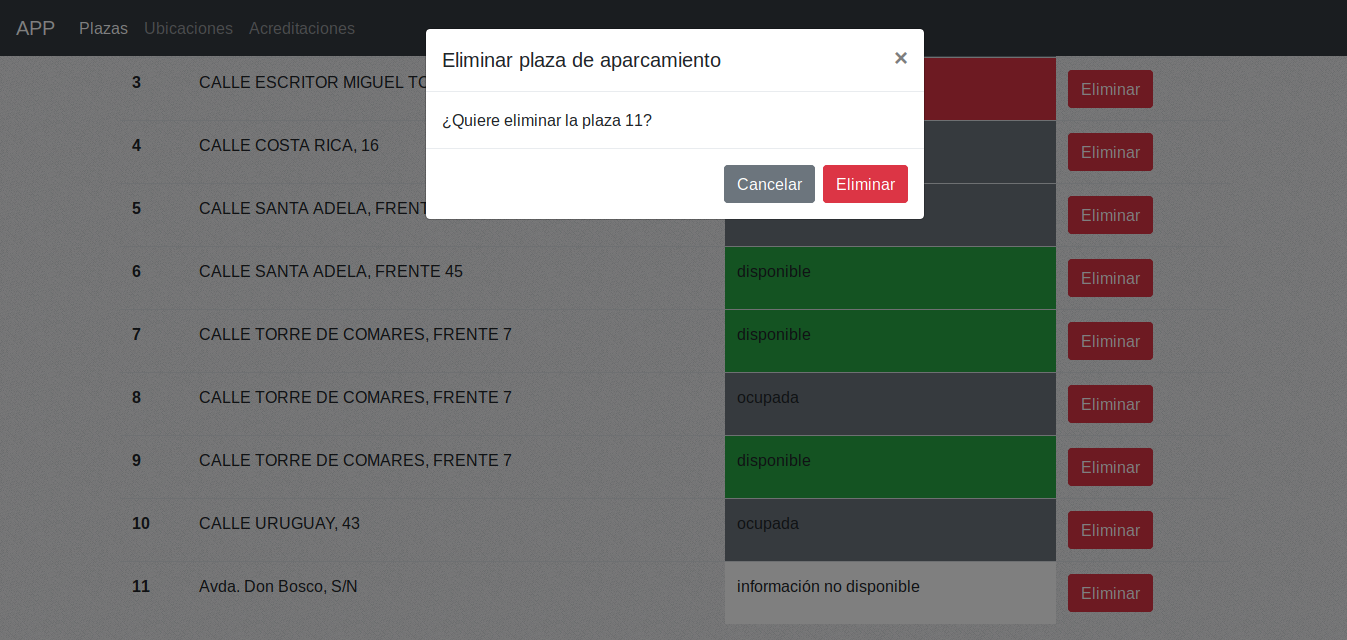
\includegraphics[width=0.9\textwidth]{imagenes/administracion/plazas_eliminar.png}
	\caption{Vista de eliminación de una plaza: aplicación de administración}
	\label{administracion_plazas_eliminar}
\end{figure}

\newpage
\subsection{Gestión de acreditaciones de aparcamiento}
Si el administrador quiere gestionar las acreditaciones de aparcamiento del sistema, debería acceder a ``acreditaciones''. Estas se ocupan de distinguir un vehículo con autorización que aparque lícitamente en una plaza reservada de uno que aparque ilícitamente.
\begin{figure}[H]
	\centering
	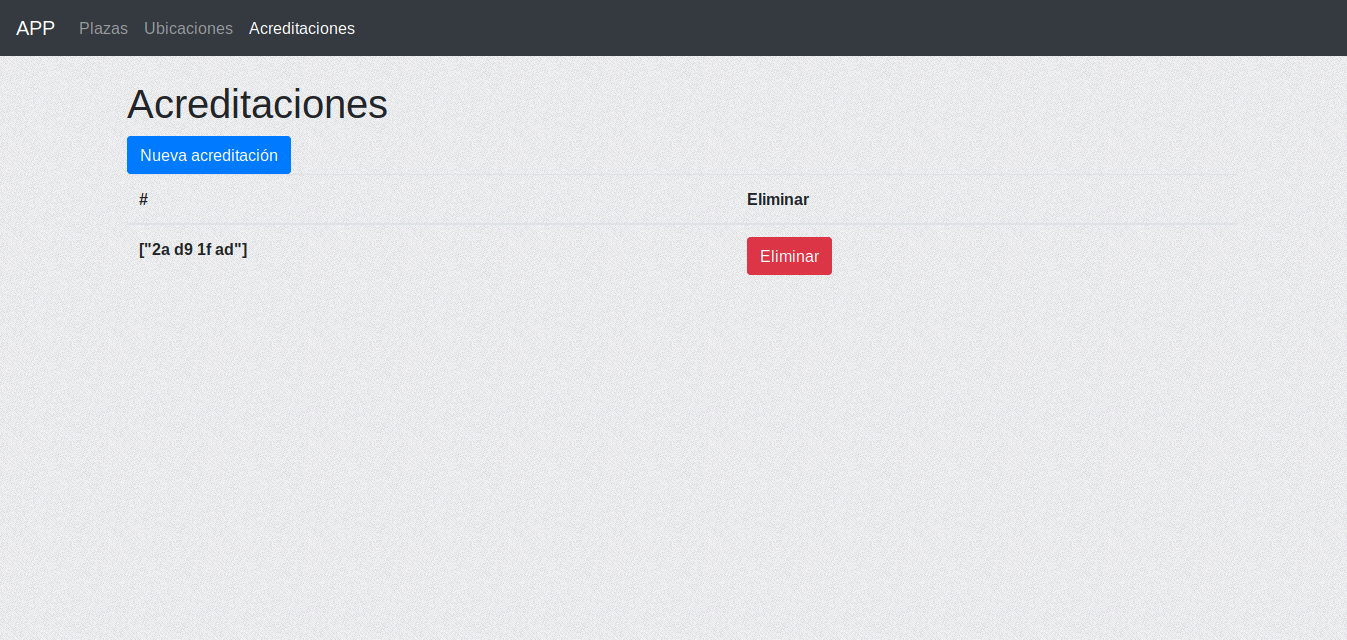
\includegraphics[width=0.9\textwidth]{imagenes/administracion/acreditaciones.png}
	\caption{Vista de acreditaciones: aplicación de administración}
	\label{administracion_acreditaciones}
\end{figure}
En esta sección, figura \ref{administracion_acreditaciones}, se pueden ver las distintas acreditaciones existentes en el sistema. Estas acreditaciones estarían vinculadas a una persona con movilidad reducida. También da la posibilidad de añadir una nueva ubicación, figura \ref{administracion_acreditaciones_nueva}, donde hay que administrarle un identificador inequívoco de la tarjeta de aparcamiento que dispone de un RFID.
\begin{figure}[H]
	\centering
	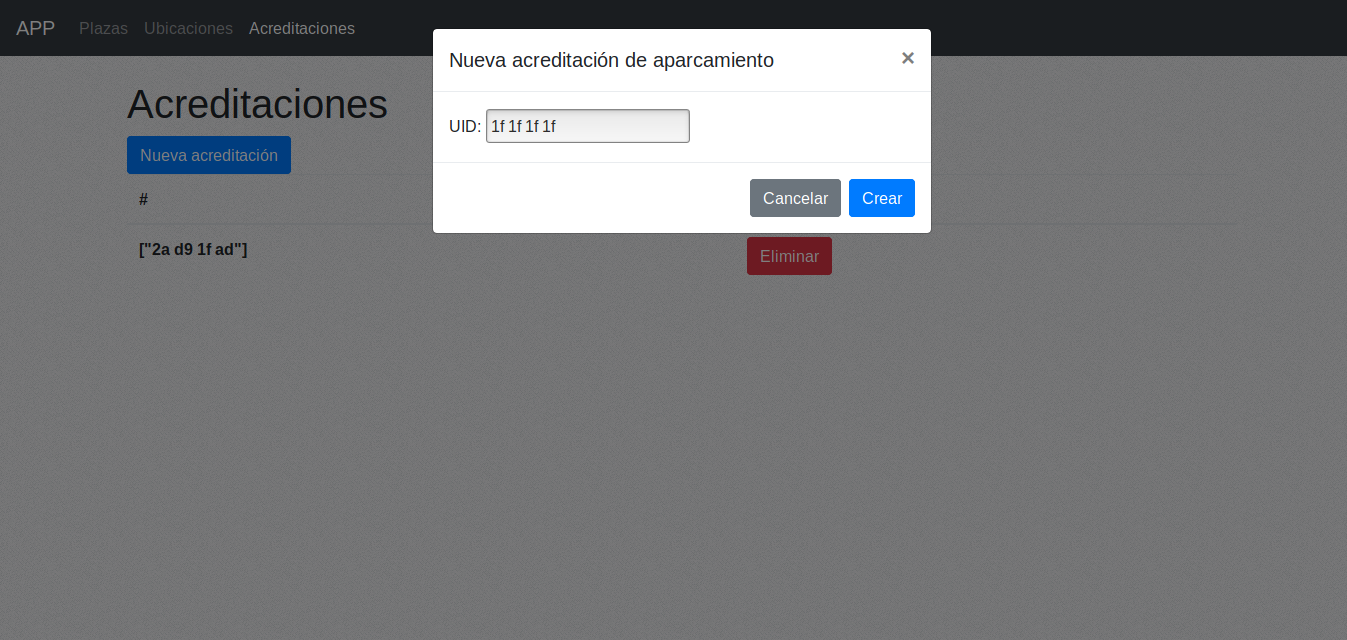
\includegraphics[width=0.9\textwidth]{imagenes/administracion/acreditaciones_nueva.png}
	\caption{Vista de creación de una nueva acreditación: aplicación de administración}
	\label{administracion_acreditaciones_nueva}
\end{figure}
Si no se indica dicho identificador, la aplicación advierte con un mensaje de error indicando que se necesita rellenar el dato obligatorio para dar de alta una nueva acreditación, figura \ref{administracion_acreditaciones_nueva_error}.
\begin{figure}[H]
	\centering
	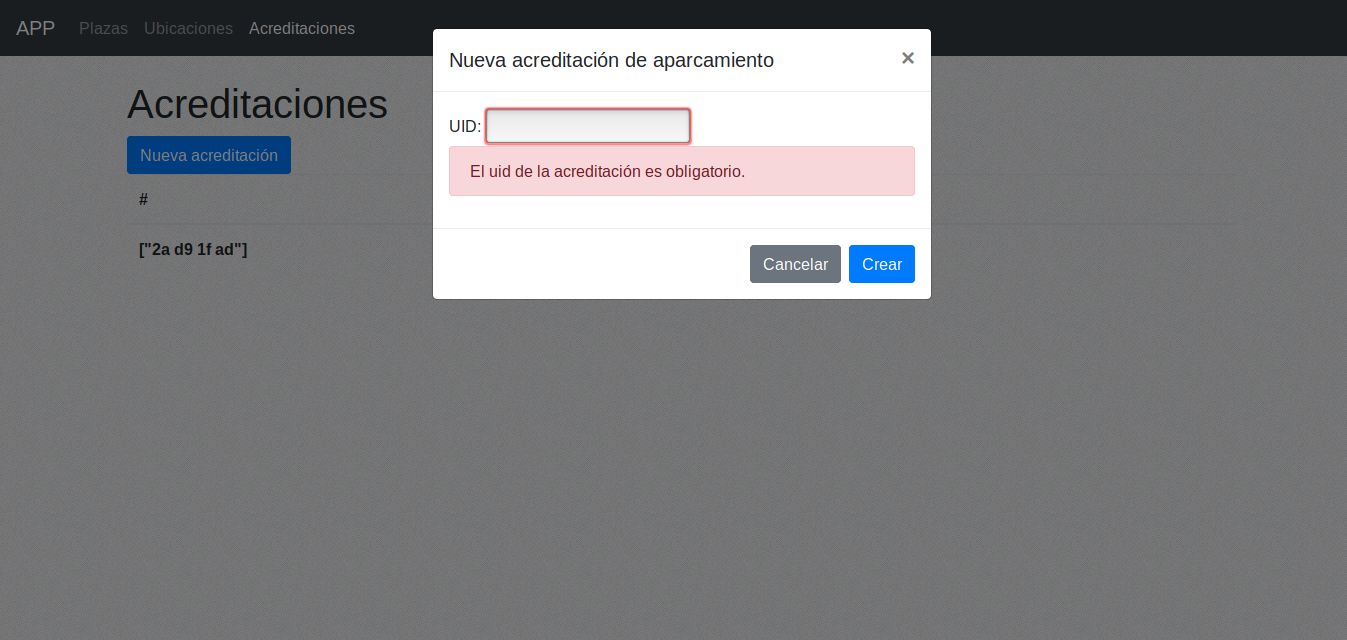
\includegraphics[width=0.9\textwidth]{imagenes/administracion/acreditaciones_nueva_error.png}
	\caption{Vista de error en la creación de una nueva acreditación: aplicación de administración}
	\label{administracion_acreditaciones_nueva_error}
\end{figure}
Si se indican correctamente el identificador para crear una nueva acreditación, el sistema añadirá la nueva acreditación, figura \ref{administracion_acreditaciones_creada}.
\begin{figure}[H]
	\centering
	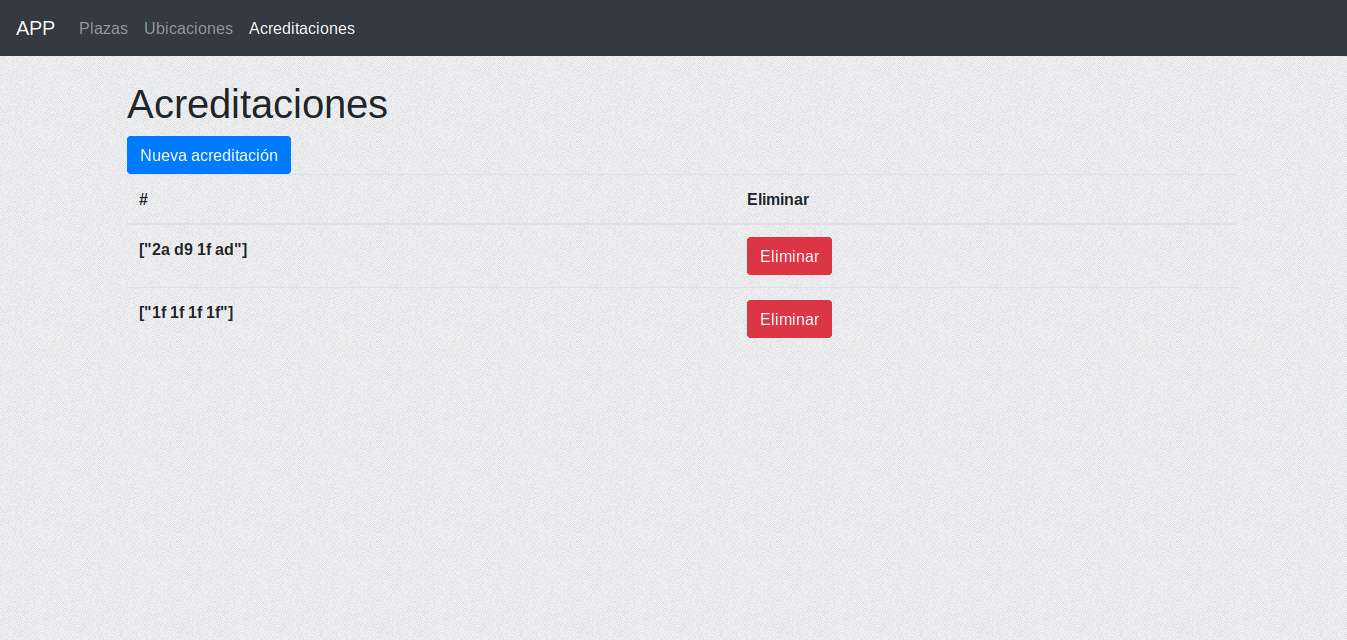
\includegraphics[width=0.9\textwidth]{imagenes/administracion/acreditaciones_creada.png}
	\caption{Vista listado con nueva acreditación: aplicación de administración}
	\label{administracion_acreditaciones_creada}
\end{figure}
En esta pantalla, junto al listado de las acreditaciones existentes, la aplicación permite eliminar de forma fácil una acreditación del sistema, figura \ref{administracion_acreditaciones_eliminar}.
\begin{figure}[H]
	\centering
	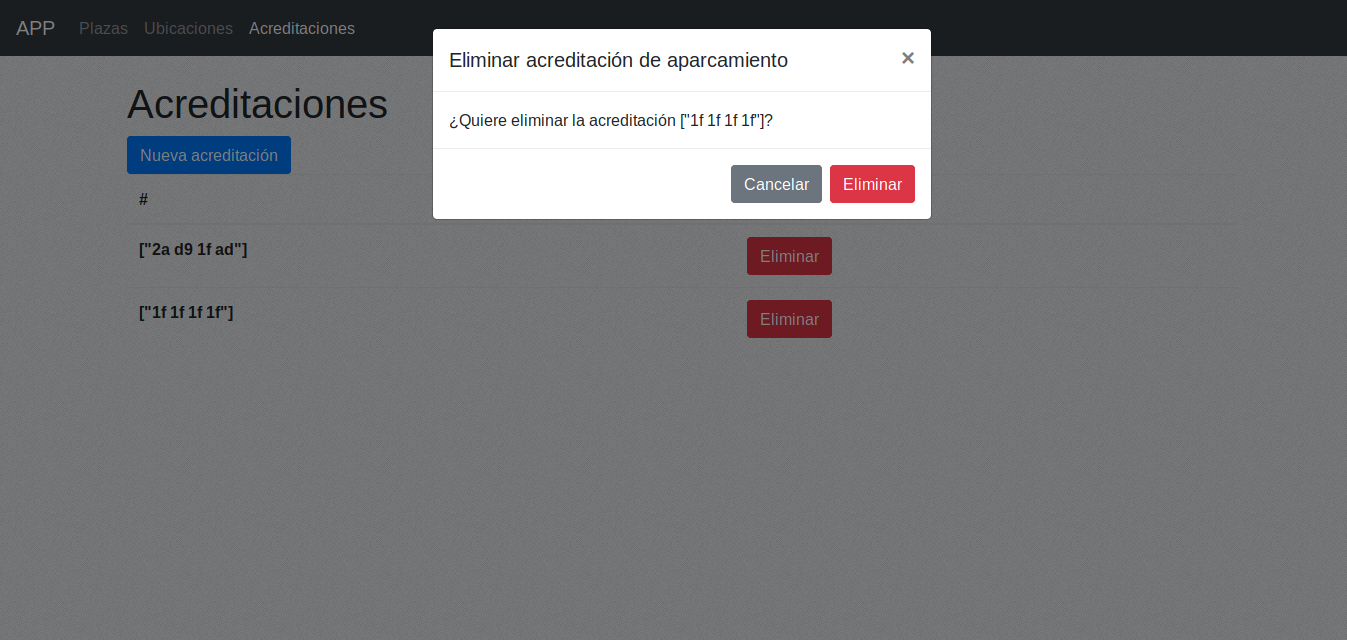
\includegraphics[width=0.9\textwidth]{imagenes/administracion/acreditaciones_eliminar.png}
	\caption{Vista de eliminación de una acreditación: aplicación de administración}
	\label{administracion_acreditaciones_eliminar}
\end{figure}

\newpage
\section{Aplicación de usuario}
La aplicación de usuario es una aplicación sencilla y amigable, diseñada para que el usuario desde su teléfono móvil, encuentre una plaza de aparcamiento cercana a su destino o se dirija a una plaza de aparcamiento que esté libre.
\begin{figure}[H]
	\centering
	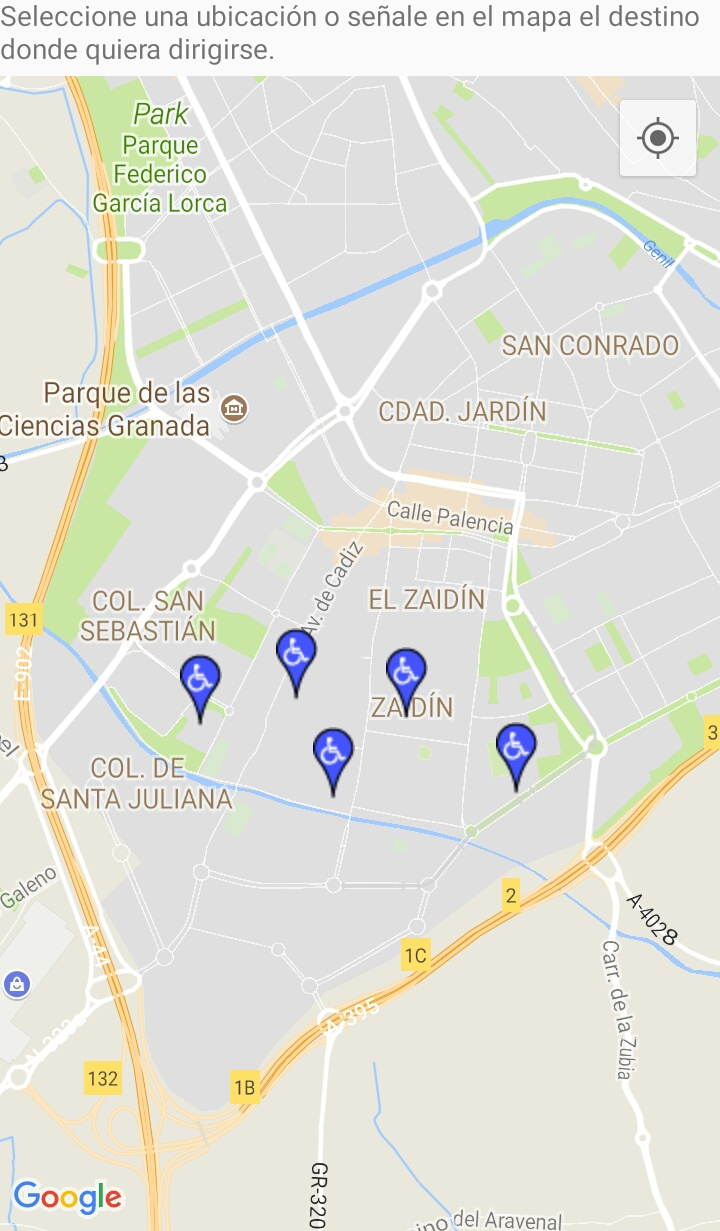
\includegraphics[width=0.4\textwidth]{imagenes/app/1.jpg}
	\caption{Vista inicial: aplicación de usuario}
	\label{app_1}
\end{figure}
Al abrir la aplicación, el usuario se encuentra un mapa donde se señalan las ubicaciones de aparcamiento, figura \ref{app_1}. Estas ubicaciones se van cargando a medida que el usuario se desplaza o amplia el mapa. Estas ubicaciones en forma de marcas en el mapa las puede señalar el usuario, apareciendo así una nueva ventana con información detallada sobre la ubicación, figura \ref{app_2}.
\begin{figure}[H]
	\centering
	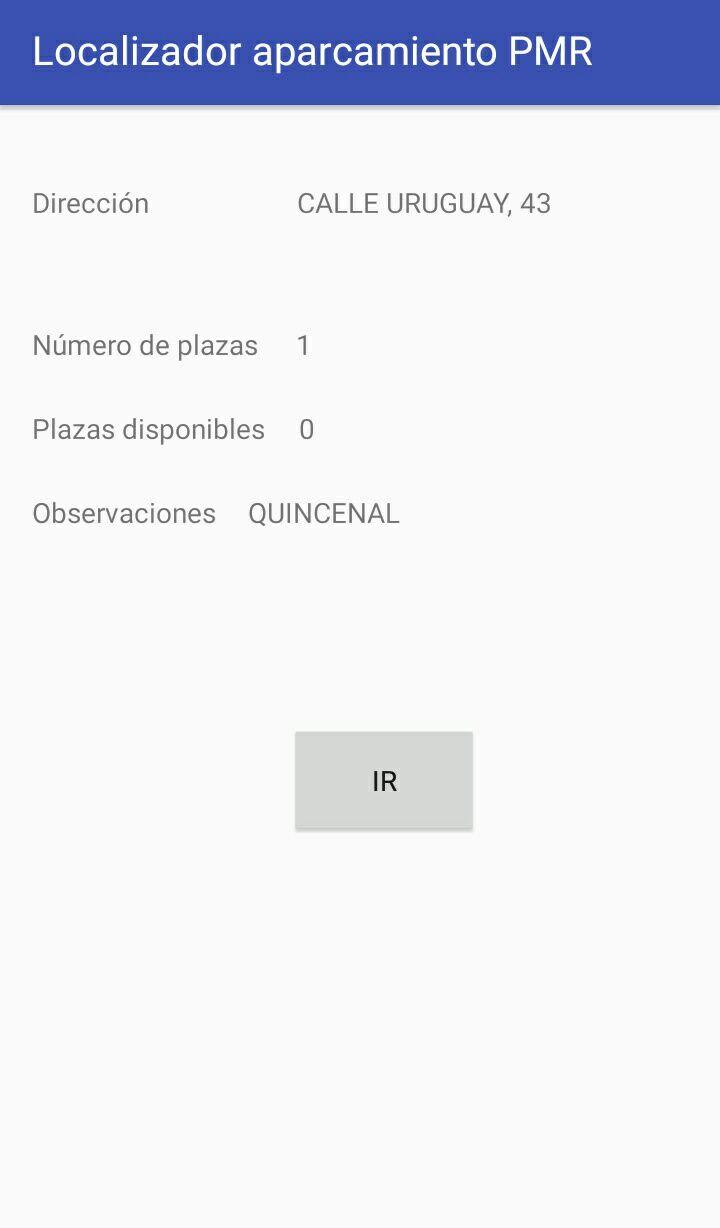
\includegraphics[width=0.4\textwidth]{imagenes/app/2.jpg}
	\caption{Vista detallada de ubicación: aplicación de usuario}
	\label{app_2}
\end{figure}
El usuario, si así lo desea, puede iniciar la navegación en automóvil hacia dicha ubicación pulsando el botón ``IR'', figura \ref{app_3}.
\begin{figure}[H]
	\centering
	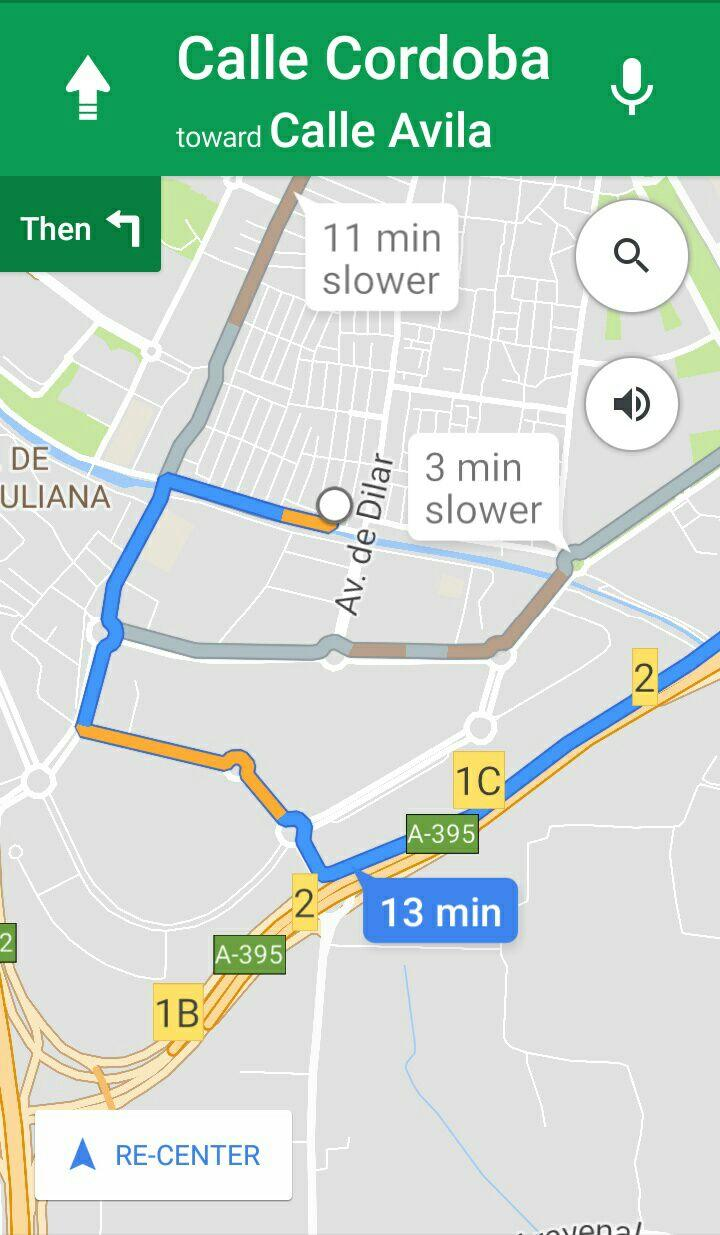
\includegraphics[width=0.4\textwidth]{imagenes/app/3.jpg}
	\caption{Vista navegación a ubicación: aplicación de usuario}
	\label{app_3}
\end{figure}
Desde el momento que inicia la navegación hasta que la finaliza, el usuario puede recibir una notificación indicándole, que la ubicación a la que se dirige, se ha quedado sin plazas libres. Dicha notificación sería:
\begin{figure}[H]
	\centering
	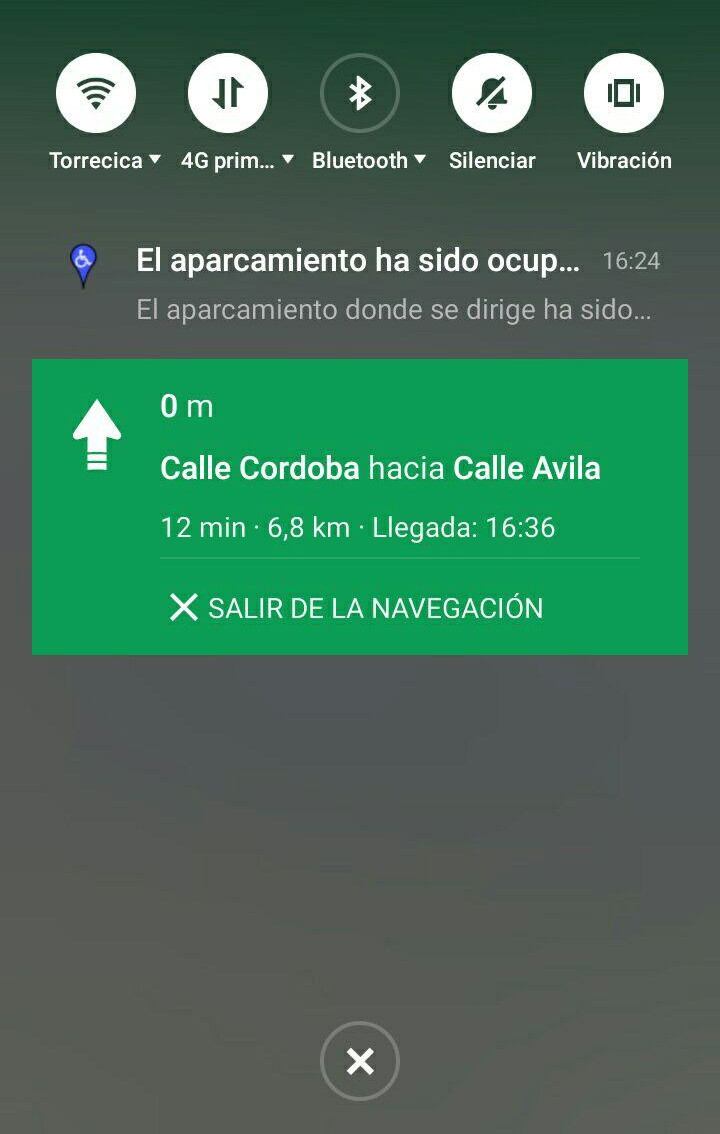
\includegraphics[width=0.4\textwidth]{imagenes/app/7.jpg}
	\caption{Vista notificación: aplicación de usuario}
	\label{app_7}
\end{figure}
Con respecto a la búsqueda de aparcamientos, el punto fuerte de esta aplicación es que el usuario puede introducir un destino pinchando en el mapa, figura \ref{app_4}.
\begin{figure}[H]
	\centering
	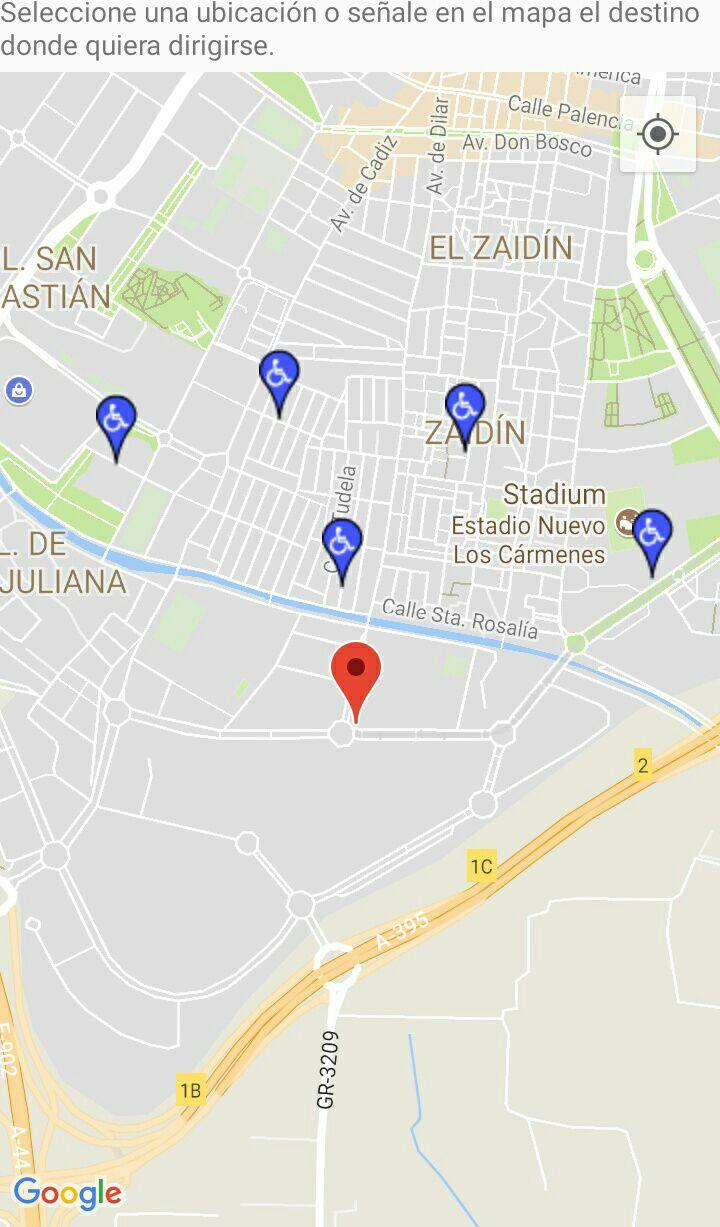
\includegraphics[width=0.4\textwidth]{imagenes/app/4.jpg}
	\caption{Vista creación de destino: aplicación de usuario}
	\label{app_4}
\end{figure}
En este momento, si el usuario mueve el mapa se borraría dicho destino. En cambie si vuelve a seleccionar su destino, la aplicación le muestra una lista de ubicaciones ordenadas por distancia al destino real del usuario donde poder aparcar, figura \ref{app_5}.
\begin{figure}[H]
	\centering
	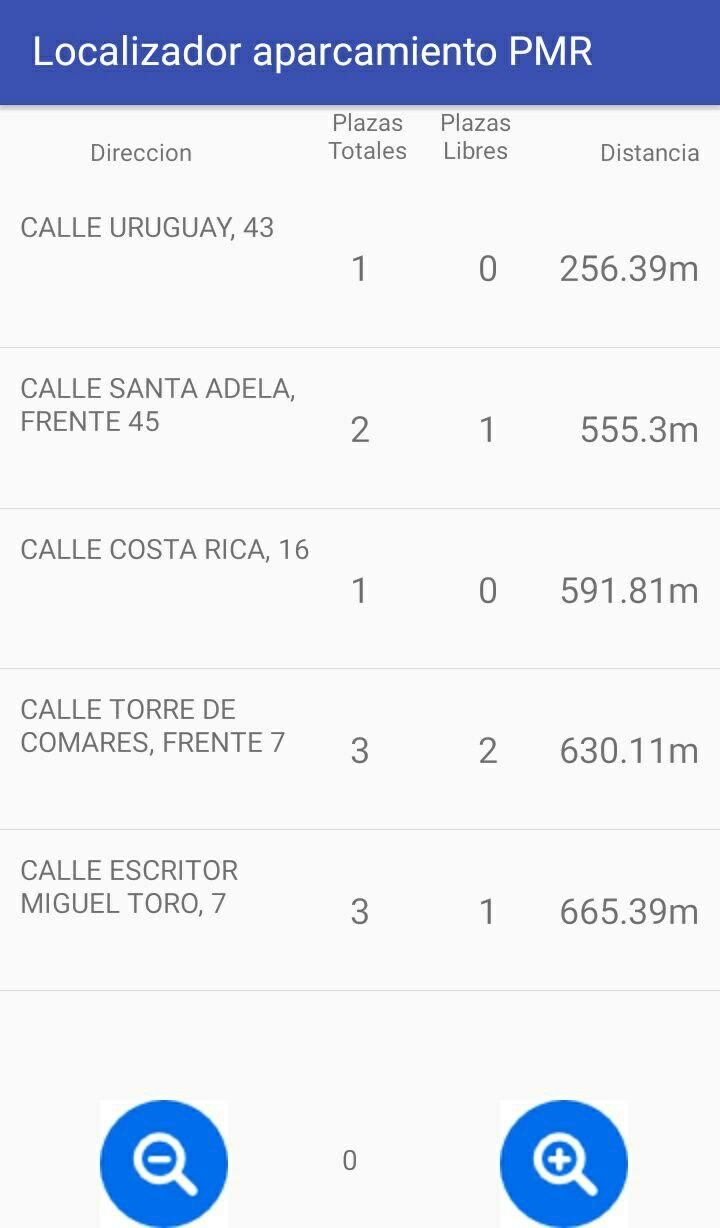
\includegraphics[width=0.4\textwidth]{imagenes/app/5.jpg}
	\caption{Vista listado de ubicaciones cercanas: aplicación de usuario}
	\label{app_5}
\end{figure}
En la lista se muestra la dirección de la plaza de aparcamiento cercana junto al número de aparcamientos que tiene, el número de ellos que están ocupados y la distancia al destino del usuario. Por otro lado, y si el usuario lo desea, puede reordenar la lista de manera que plazas más lejanas, con mayor número de aparcamientos libres, salgan en primeras posiciones. Por ello, en la parte inferior de la pantalla se han puesto dos botones de búsqueda.
\begin{figure}[H]
	\centering
	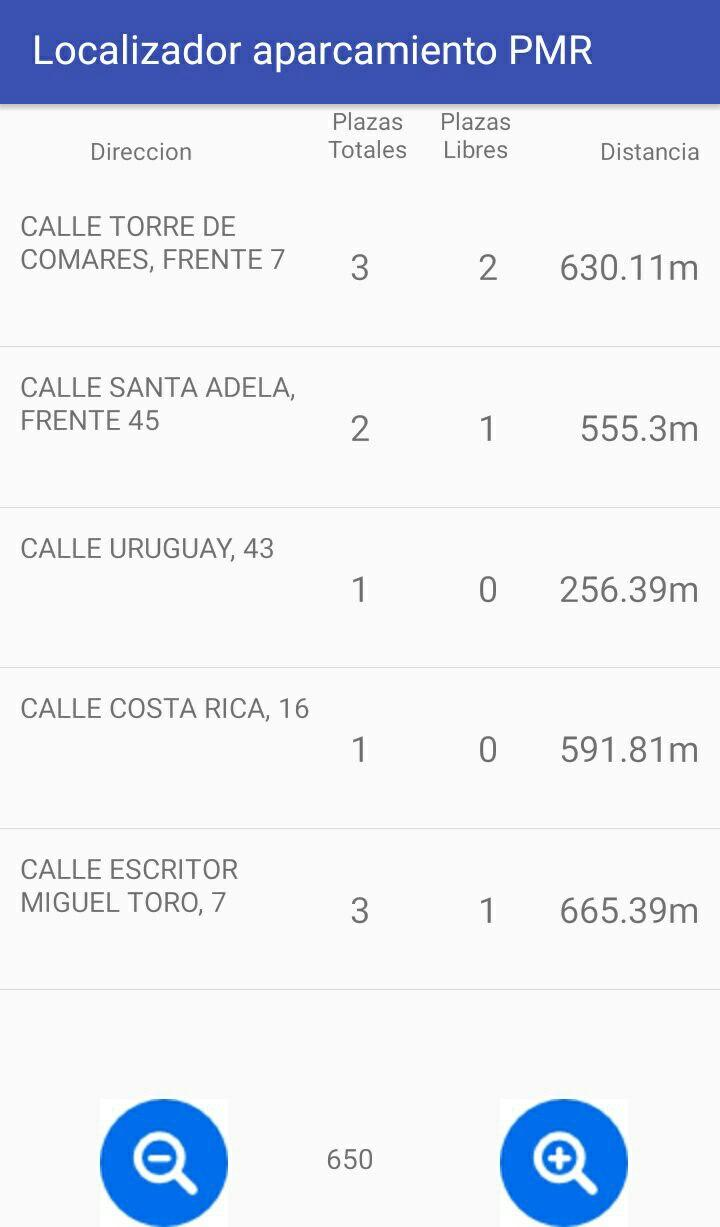
\includegraphics[width=0.4\textwidth]{imagenes/app/6.jpg}
	\caption{Vista listado de ubicaciones cercanas agrupado por distancias: aplicación de usuario}
	\label{app_6}
\end{figure}
Pulsando sobre el ``+'' la distancia que aparece entre los botones aumenta y las plazas se actualizan y ordenan. Es la  forma que tiene el usuario para decirle a la aplicación la distancia que estaría dispuesto a recorrer.
\\\\
Si el usuario selecciona un destino, la aplicación entraría en modo navegación al igual que anteriormente, figura \ref{app_3} haciendo uso de la aplicación Google Maps de Android.
\chapter{Conclusiones y Trabajo Futuro}
Desde el punto de vista de la solución alcanzada, como se ha podido ver en este trabajo, se han desarrollado tres prototipos software (API REST, aplicación de administración y aplicación de usuario) y uno hardware (agente de captación de datos). El sistema que se ha desarrollado es una prueba de concepto y, a su vez, un producto mínimo viable (PMV) que aúne estos cuatro prototipos para dar solución a un problema real de la sociedad.
\\\\
Desde el punto de vista académico, por un lado se ha puesto de manifiesto que se ha analizado un problema real junto con sus restricciones y se ha combinado el conocimiento con la técnica adecuada para proponer un sistema completo de tal calibre. Como dicho análisis queda grande en el contexto de un TFG, se ha procedido a reducir dicho sistema completo en otro que, a su vez, es completamente funcional.
\\\\
Por otro lado, la implementación y la creación del prototipo hardware han sido posibles tras un minucioso estudio de distintas tecnologías dentro del ámbito TICs. A su vez, se ha querido encontrar aquellas tecnologías que resuelven el problema de la mejor manera posible sin necesitar demasiados recursos. Esto se traduce en que se ha puesto un elevado interés para intentar que el sistema desarrollado sea viable en un futuro.
\\\\
También, desde el punto de vista personal, la creación de este proyecto ha sido una gran satisfacción al ver que he tenido los conocimientos, técnicas y autodeterminación necesarias para poder abordar un problema real que, al igual que a mí, afecta a un colectivo de personas. Dicho esto último, tras analizar soluciones similares, haber creado un PMV puede abrirme un futuro laboral inesperado.
\\\\
Sabiendo que se ha tenido que hacer una adaptación, que realmente es el núcleo principal, de un sistema ideal de gestión de aparcamientos para PMR, ha quedado un gran desarrollo para el futuro. Este trabajo no es sólo de desarrollo de algunas funcionalidades que, por el marco de este trabajo, no se han podido implementar sino, a su vez, se ha quedado un trabajo de investigación para predecir el estado de las ubicaciones para una mejor experiencia del usuario.
\\\\
Además, debido a que se ha estudiado el marco legal del problema a nivel Europeo, esta solución puede expandirse a otros países dando pie a un desarrollo todavía mayor.

\appendix
\chapter{Listado de URIs de la API REST}
A continuación se desglosan las funcionalidades de la API REST que se han creado para que el sistema funcione:
\begin{itemize}
	\item URIs referentes a plazas:
	\begin{itemize}
		\item \textit{/plazas}, con método GET, devuelve un listado con las plazas existentes en el sistema.
		\item \textit{/plaza/<id>}, con método GET, devuelve el objeto plaza cuyo identificador es \textit{<id>}.
		\item \textit{/plaza/nueva}, con método POST, añade una plaza al sistema. Necesita del parámetro obligatorio \textit{id\_ubicacion}, identificador de una ubicación existente en el sistema.
		\item \textit{/plaza/<id>/estado/<estado>}, con método PUT, cambia el estado de la plaza cuyo identificador es \textit{<id>} al nuevo estado \textit{<estado>}.
		\item \textit{/plaza/<id>}, con método DELETE, elimina la plaza existente cuyo identificador es \textit{<id>} del sistema.
		\item \textit{/plazas/mal\_ocupadas}, con método GET, devuelve un listado de plazas cuyo estado es \textit{mal ocupada}.
	\end{itemize}
	\item URIs referentes a ubicaciones:
	\begin{itemize}
			\item \textit{/ubicaciones}, con método GET, devuelve un listado con las ubicaciones existentes en el sistema.
		\item \textit{/ubicaciones/<lat\_min>\&<lat\_max>/<long\_min>\&<long\_max>}, con método GET, devuelve un listado de ubicaciones que se encuentran geoposicionadas dentro de un área cuyos límites son: \textit{<lat\_min>}, \textit{<long\_min>} y \textit{<lat\_max>}, \textit{<long\_max>}.
		\item \textit{/ubicaciones/<lat>\&<long>}, con método GET, devuelve un listado de ubicaciones ordenado por distancia a la posición cuyas coordenadas son \textit{<lat>}, \textit{<long>} (latitud y longitud respectivamente).
		\item \textit{/ubicaciones/<lat>\&<long>/<grano>}, con método GET, devuelve un listado de ubicaciones ordenado por distancia a la posición cuyas coordenadas son \textit{<lat>}, \textit{<long>} (latitud y longitud respectivamente) y número de plazas libres en grupos de ubicaciones que se encuentren en tramos de distancia de \textit{<grano>}.
		\item \textit{/ubicacion/<id>}, con método GET, devuelve un los campos de la ubicación cuyo identificador en \textit{<id>}.
		\item \textit{/ubicacion/nueva}, con método POST, añade una nueva ubicación al sistema. Necesita de los parámetros obligatorios; \textit{direccion} calle y número de la ubicación, \textit{latitud} y \textit{longitud} coordenadas de la ubicación. El parámetro \textit{observaciones} no es obligatorio e indica cualquier aclaración sobre la ubicación.
		\item \textit{/ubicacion/<id>}, con método DELETE, elimina la ubicación existente cuyo identificador es \textit{<id>} del sistema.
		\item \textit{/ubicacion/<id>}, con método POST, modifica la ubicación existente en el sistema cuyo identificador es \textit{<id>}. Recibe los parámetros: \textit{direccion} de forma obligatoria y \textit{observaciones}.
	\end{itemize}
	\item URIs referentes a acreditaciones:
	\begin{itemize}
		\item \textit{/acreditaciones}, con método GET, devuelve un listado con las acreditaciones existentes en el sistema.
		\item \textit{/acreditacion/nueva}, con método POST, añade una nueva acreditación en el sistema. Necesita el parámetro obligatorio \textit{uid} que es el identificador de la ubicación.
		\item \textit{/acreditacion/<uid>}, con método GET, comprueba si existe la acreditación cuyo identificador es \textit{<uid>} en el sistema.
		\item \textit{/acreditacion/<uid>}, con método DELETE, elimina la acreditación existente cuyo identificador es \textit{<uid>} del sistema.
	\end{itemize}
	\item URIs referentes a notificaciones para aplicación móvil:
	\begin{itemize}
			\item \textit{/destino\_activo/nueva}, con método POST, añade un nuevo destino activo en el sistema.\\ Necesita de los parámetros obligatorios: \textit{id\_ubicación} identificador de una ubicación existente en el sistema y \textit{token} identificador del dispositivo del usuario.
		\item \textit{/destino\_activo/<token>}, con método DELETE, elimina el destino activo asociado al dispositivo del usuario cuyo identificador es \textit{<token>} del sistema.
	\end{itemize}
	\newpage
	\item URIs referentes al destino final de los usuarios:
	\begin{itemize}
		\item \textit{/destinos\_usuario/nueva<lat>\&<long>}, con método PUT, añade un nuevo destino final de coordenadas \textit{<lat>} y \textit{long}, latitud y longitud, al sistema.
	\end{itemize}
\end{itemize}
\chapter{Población de la base de datos}
Para comprobar que el sistema que se ha creado funciona correctamente, se necesita suministrarlo de datos. Dichos datos suelen ser creados expresamente para probar el sistema. En este caso se ha decidido usar datos reales de las plazas para PMR de la ciudad de Granada.
\\\\
En primer lugar se ha tenido que encontrar una fuente de información de donde poder sacar los datos reales. Por suerte, Granada cuenta con una página web \cite{movilidad} donde los habitantes y visitantes de esta ciudad pueden encontrar información relativa a tráfico, zonas restringidas, transporte público o aparcamiento entre otra información.
\\\\
Dentro de la parte de \textit{aparcamiento} se puede encontrar otra página con información expresa para plazas para PMR. Dicha página cuenta con un mapa donde poder localizar las plazas, así como un listado de las mismas. También, adjunta un documento \textit{KMZ} para descargar la información de las plazas de aparcamiento.
\\\\
Este tipo de documento es un archivo comprimido que contiene, como base principal, un documento \textit{KML} \cite{kml}. Como se explica en la referencia, dicho tipo de documento es un estándar para almacenar información relativa a datos de carácter geolocalizados.
\\\\
Para extraer y poblar al sistema con estos datos, se ha necesitado hacer un programa que analice y extraiga la información que necesita el sistema del documento \textit{KML}. Una vez extraída la información, con ayuda de otro programa que hace llamadas a las distintas URIs de la API REST, se ha logrado dar de alta esta información en el sistema.
\\\\
En conclusión y para automatizar esta labor, estos programas se pueden ejecutar de forma automática a través de un procedimiento, \textit{script}, que primero descarga el archivo \textit{KMZ} de la página web oficial y lo descomprime. Luego llama a los programas anteriormente descritos para extraer la información necesitada y añadir dicha información al sistema.
\\\\
También, en este último procedimiento se puede especificar, si se quiere, el número de ubicaciones a añadir en el sistema para, por ejemplo, probar su funcionamiento. A su vez, si se indica, el estado de las plazas de las ubicaciones que se creen en el sistema tomaría valor. En caso contrario, al crear una plaza, por defecto, su estado es ``Información no disponible''.
\\\\
Para probar esta serie de procedimientos y el sistema que se ha creado, se va a poblar la base de datos con todos los aparcamientos de la ciudad de Granada.
%\begin{figure}[H]
%	\centering
%	\includegraphics[width=\textwidth]{imagenes/administracion_poblacion.png}
%	\caption{Población de la base de datos. Vista de ubicaciones: aplicación de administración}
%	\label{administracion_poblacion}
%\end{figure}
%\begin{figure}[H]
%	\centering
%	\includegraphics[width=0.35\textwidth]{imagenes/app_poblacion.jpg}
%	\caption{Vista listado de ubicaciones cercanas: aplicación de usuario}
%	\label{app_poblacion}
%\end{figure}
Tal y como se puede ver en las figuras \ref{administracion_poblacion} y \ref{app_poblacion}, el sistema ya tiene cargadas todas las plazas de Granada. El número de plazas que está soportando es 836, distribuidas en 524 ubicaciones.


\newpage

\bibliographystyle{unsrt}
\bibliography{citas}
\end{document}